\clearpage
\setcounter{chapter}{0}
\renewcommand{\thechapter}{P\arabic{chapter}}
\renewcommand{\theHchapter}{provenance.\arabic{chapter}}
\ifBookArchive
\chapter{Source inventory}\label{source-inventory}

All 426 archived source documents in this edition are included. The inventory records the exact UTF-8 source SHA-256 for each chapter. Repository planning prose is historical design evidence; GitHub issues and milestones own current scope. Retired-document links resolve to the archived base revision.

The numeric chapter field below identifies the corresponding R record: 1 means R1, and so on. Physical pagination differs between the standalone archive and complete edition.

\begin{center}
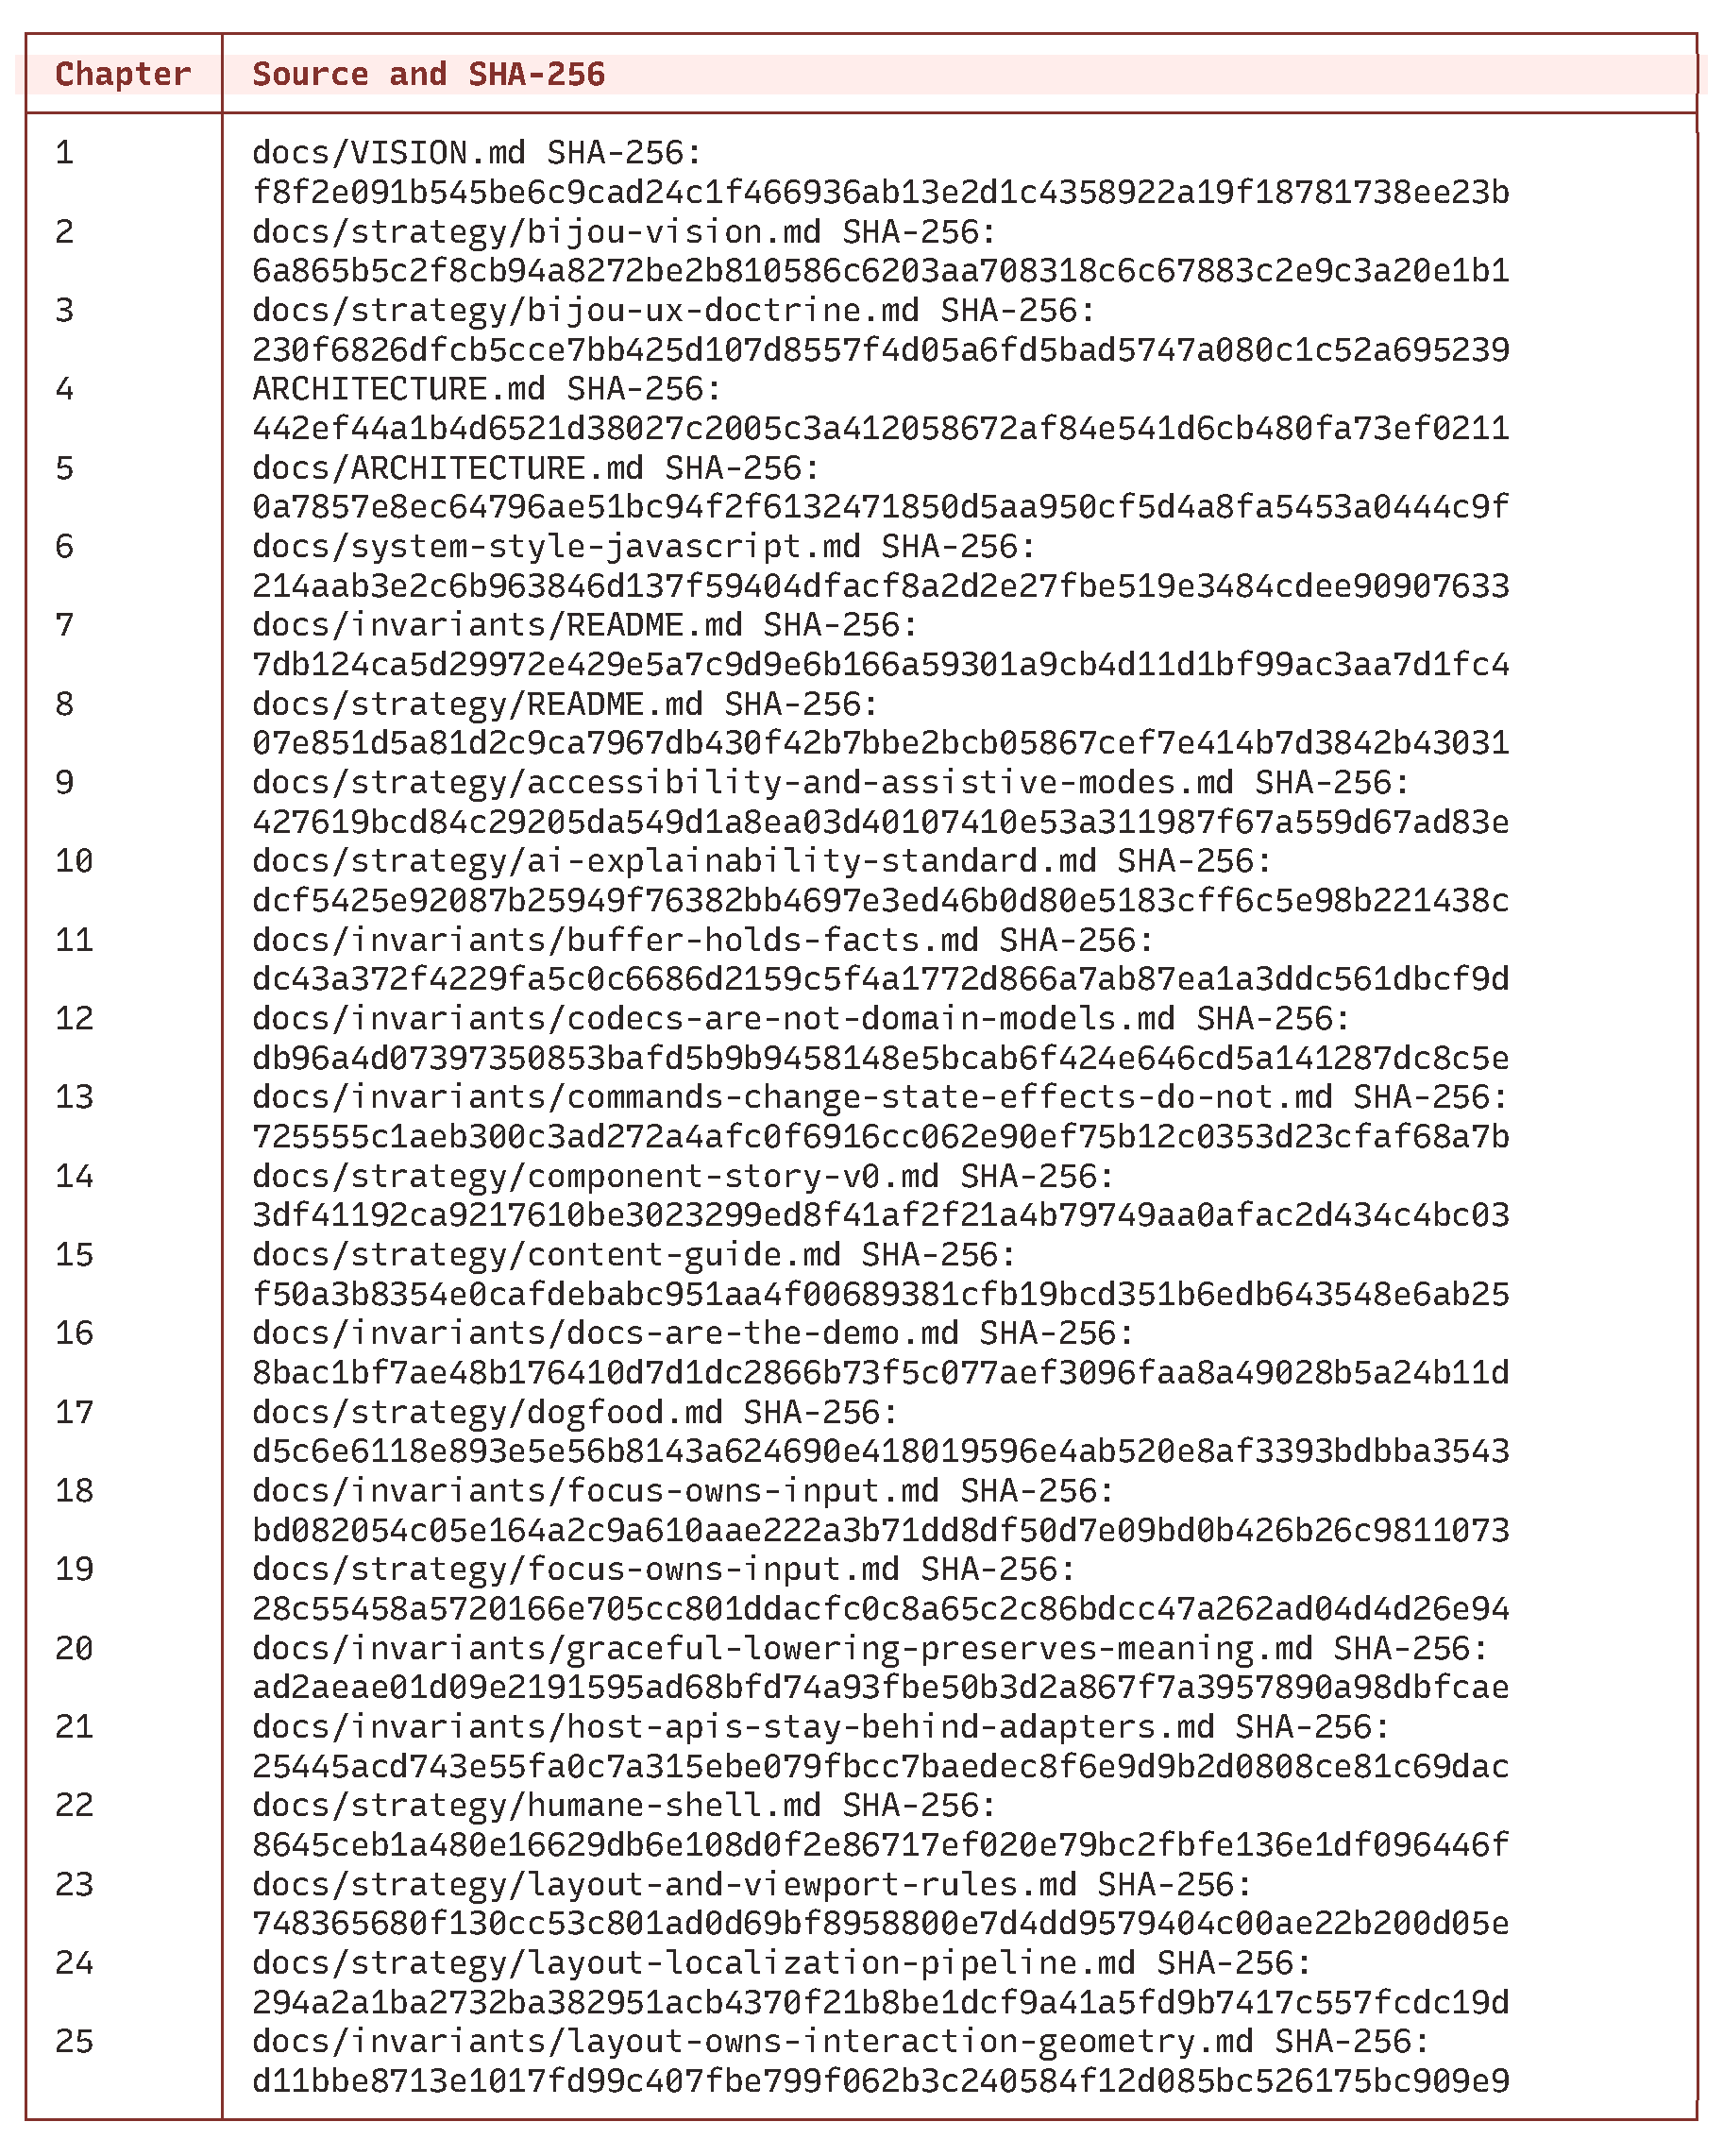
\includegraphics[width=\linewidth]{figures/tables/source-inventory-g1-1.pdf}
\par\smallskip{\scriptsize\color{BookMuted}Rows 1–25. Actual Bijou table component.}
\end{center}
\par\medskip
\begin{center}
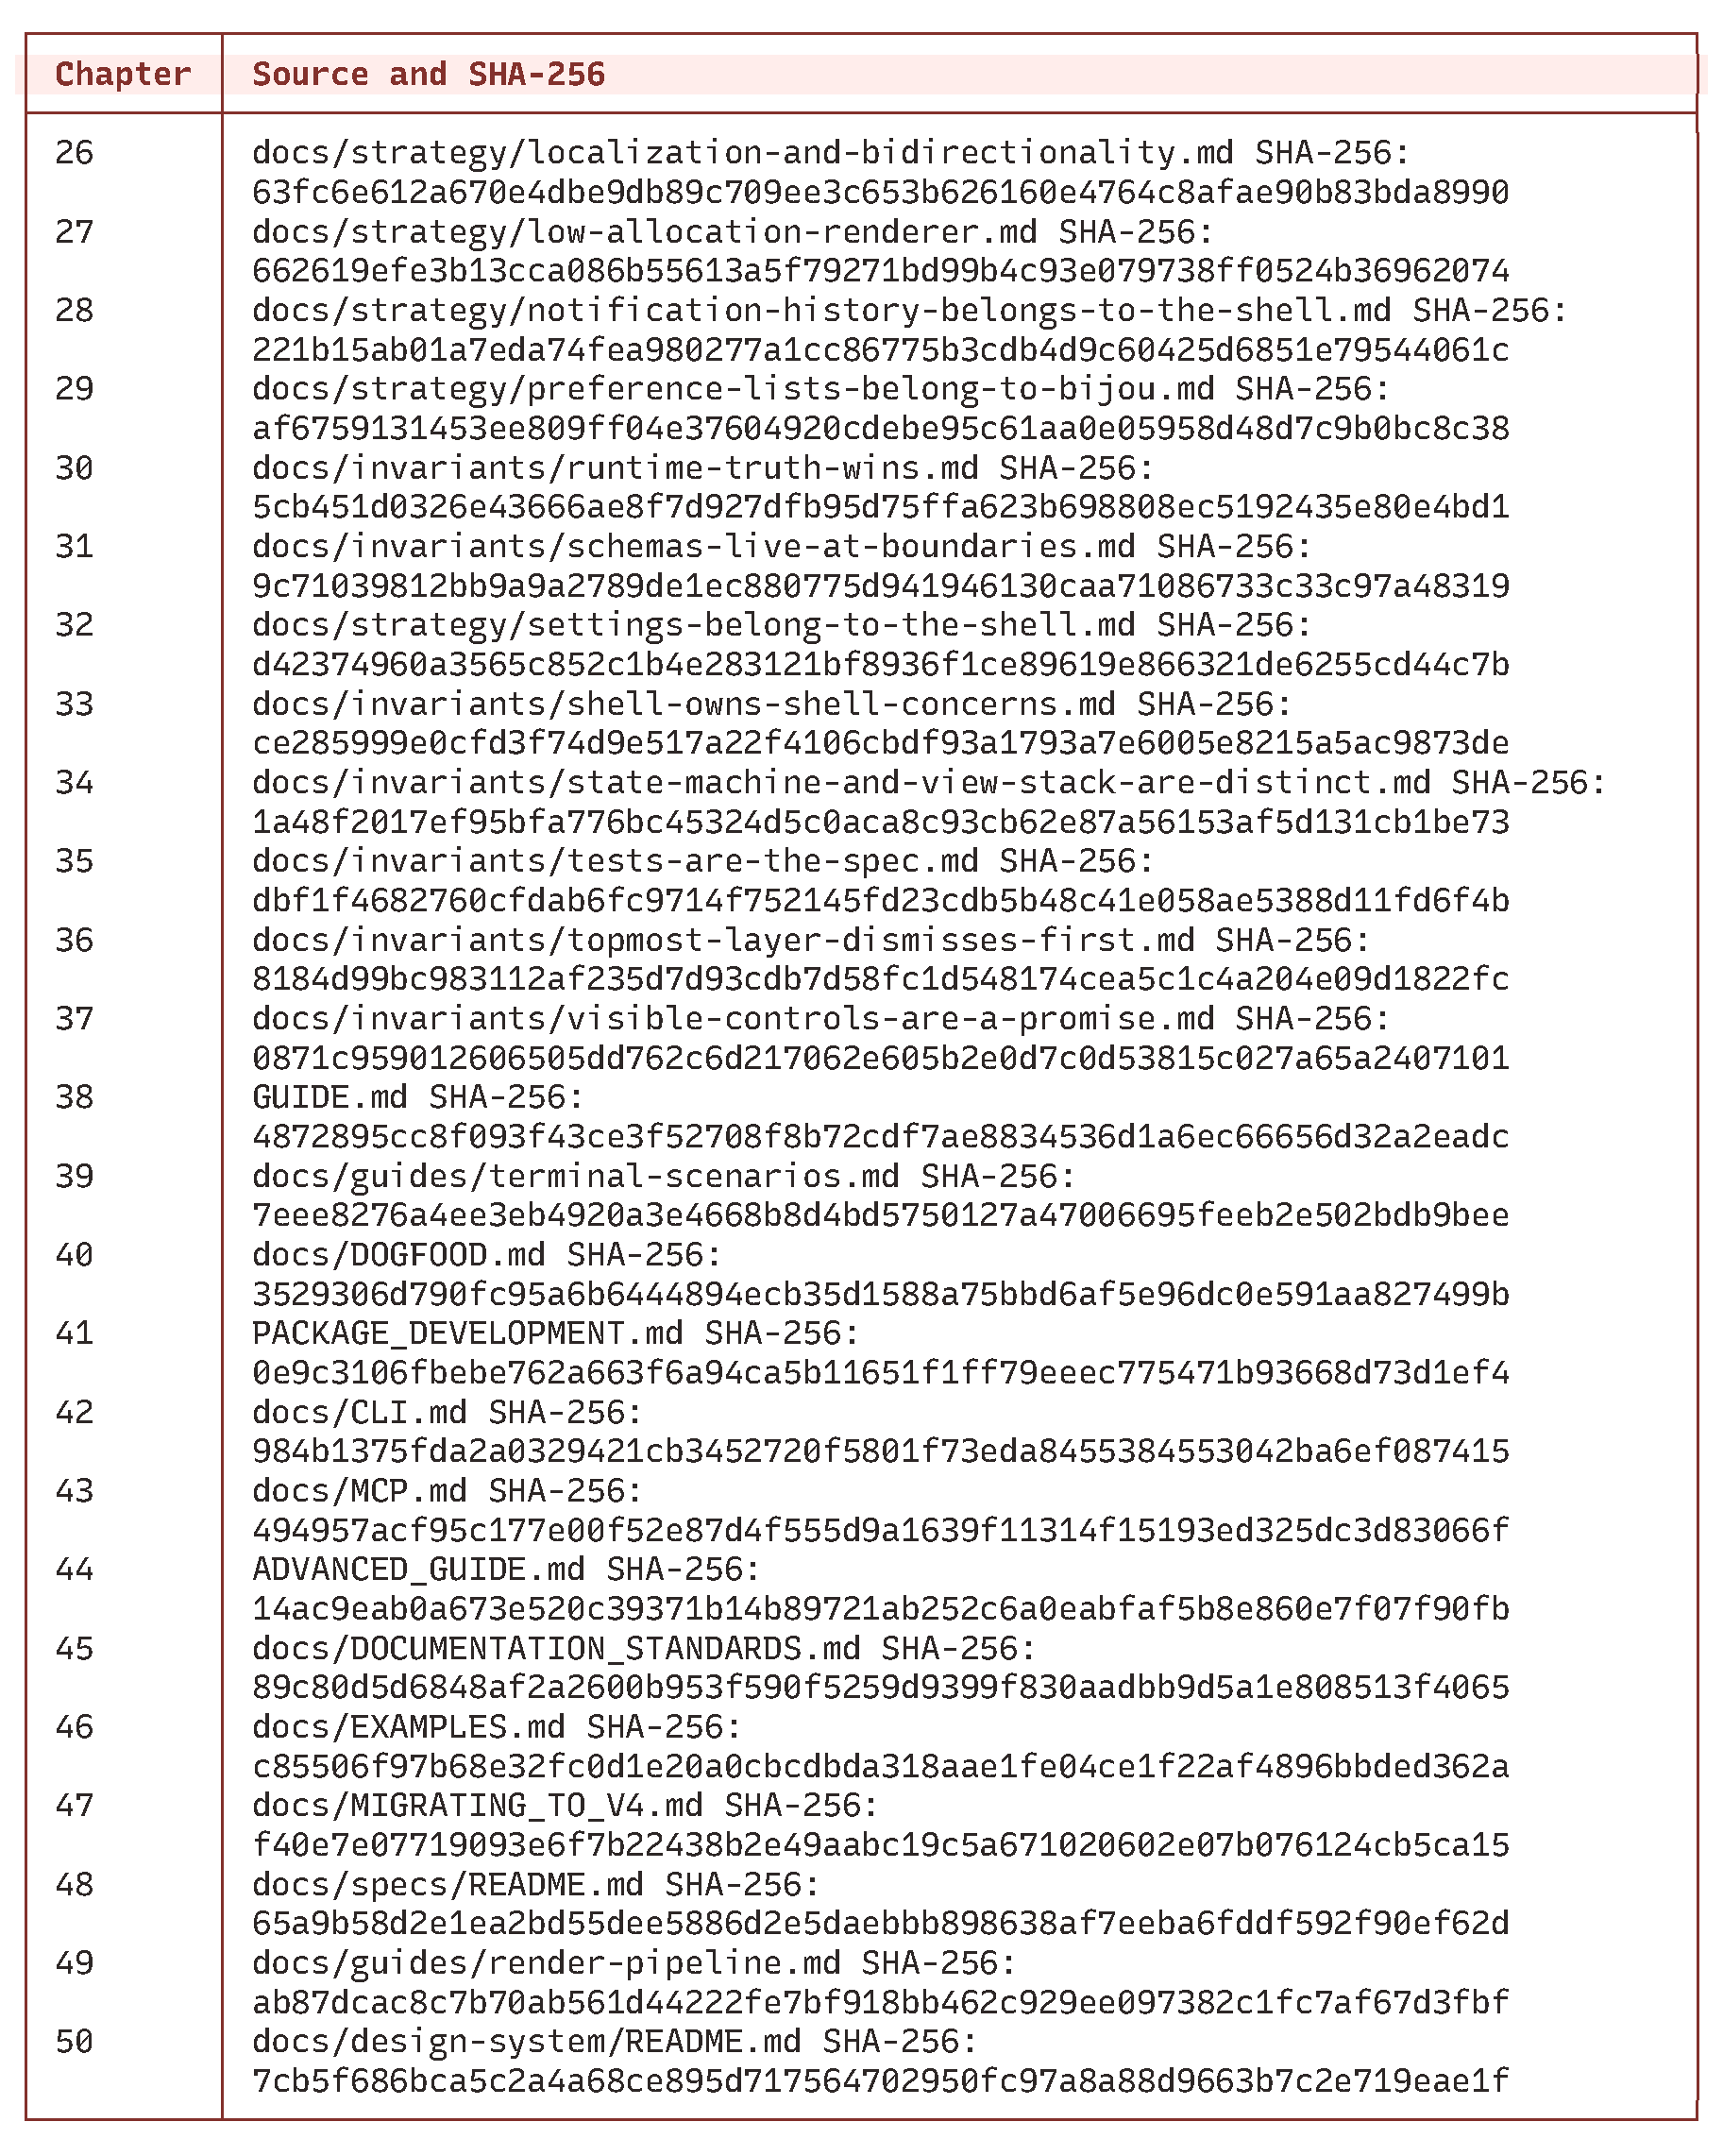
\includegraphics[width=\linewidth]{figures/tables/source-inventory-g1-2.pdf}
\par\smallskip{\scriptsize\color{BookMuted}Rows 26–50. Actual Bijou table component.}
\end{center}
\par\medskip
\begin{center}
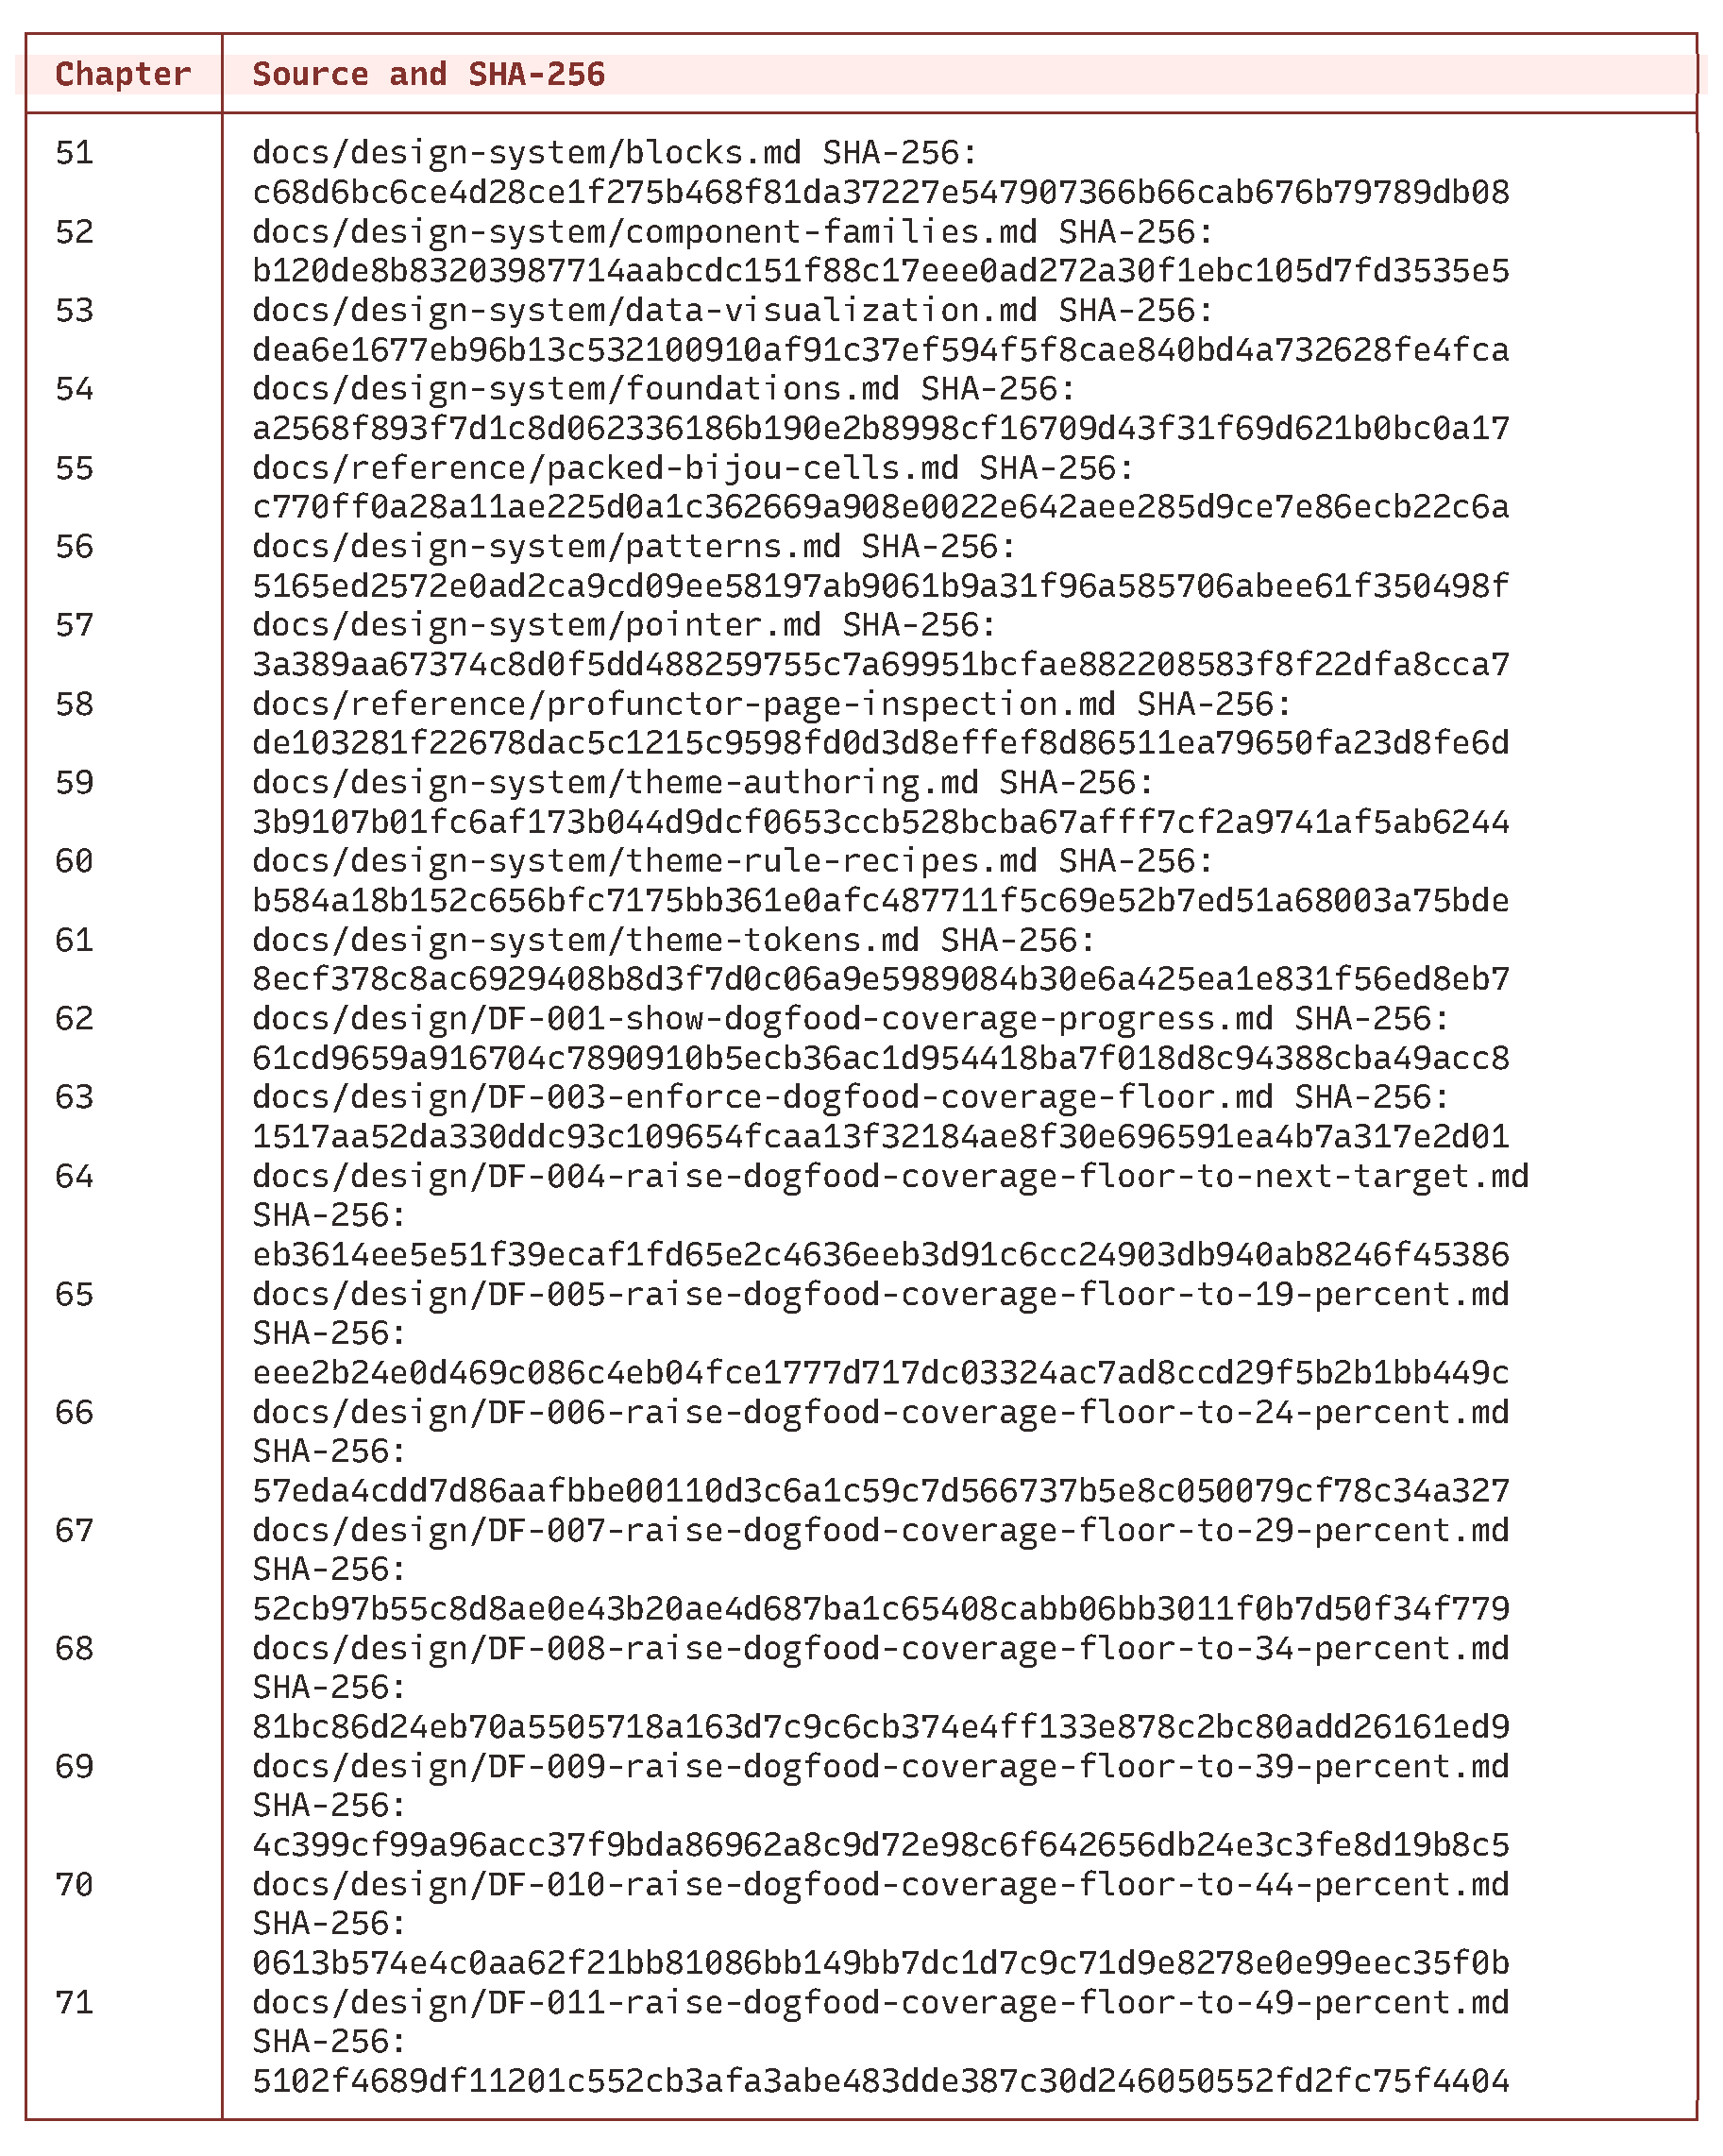
\includegraphics[width=\linewidth]{figures/tables/source-inventory-g1-3.pdf}
\par\smallskip{\scriptsize\color{BookMuted}Rows 51–71. Actual Bijou table component.}
\end{center}
\par\medskip
\begin{center}
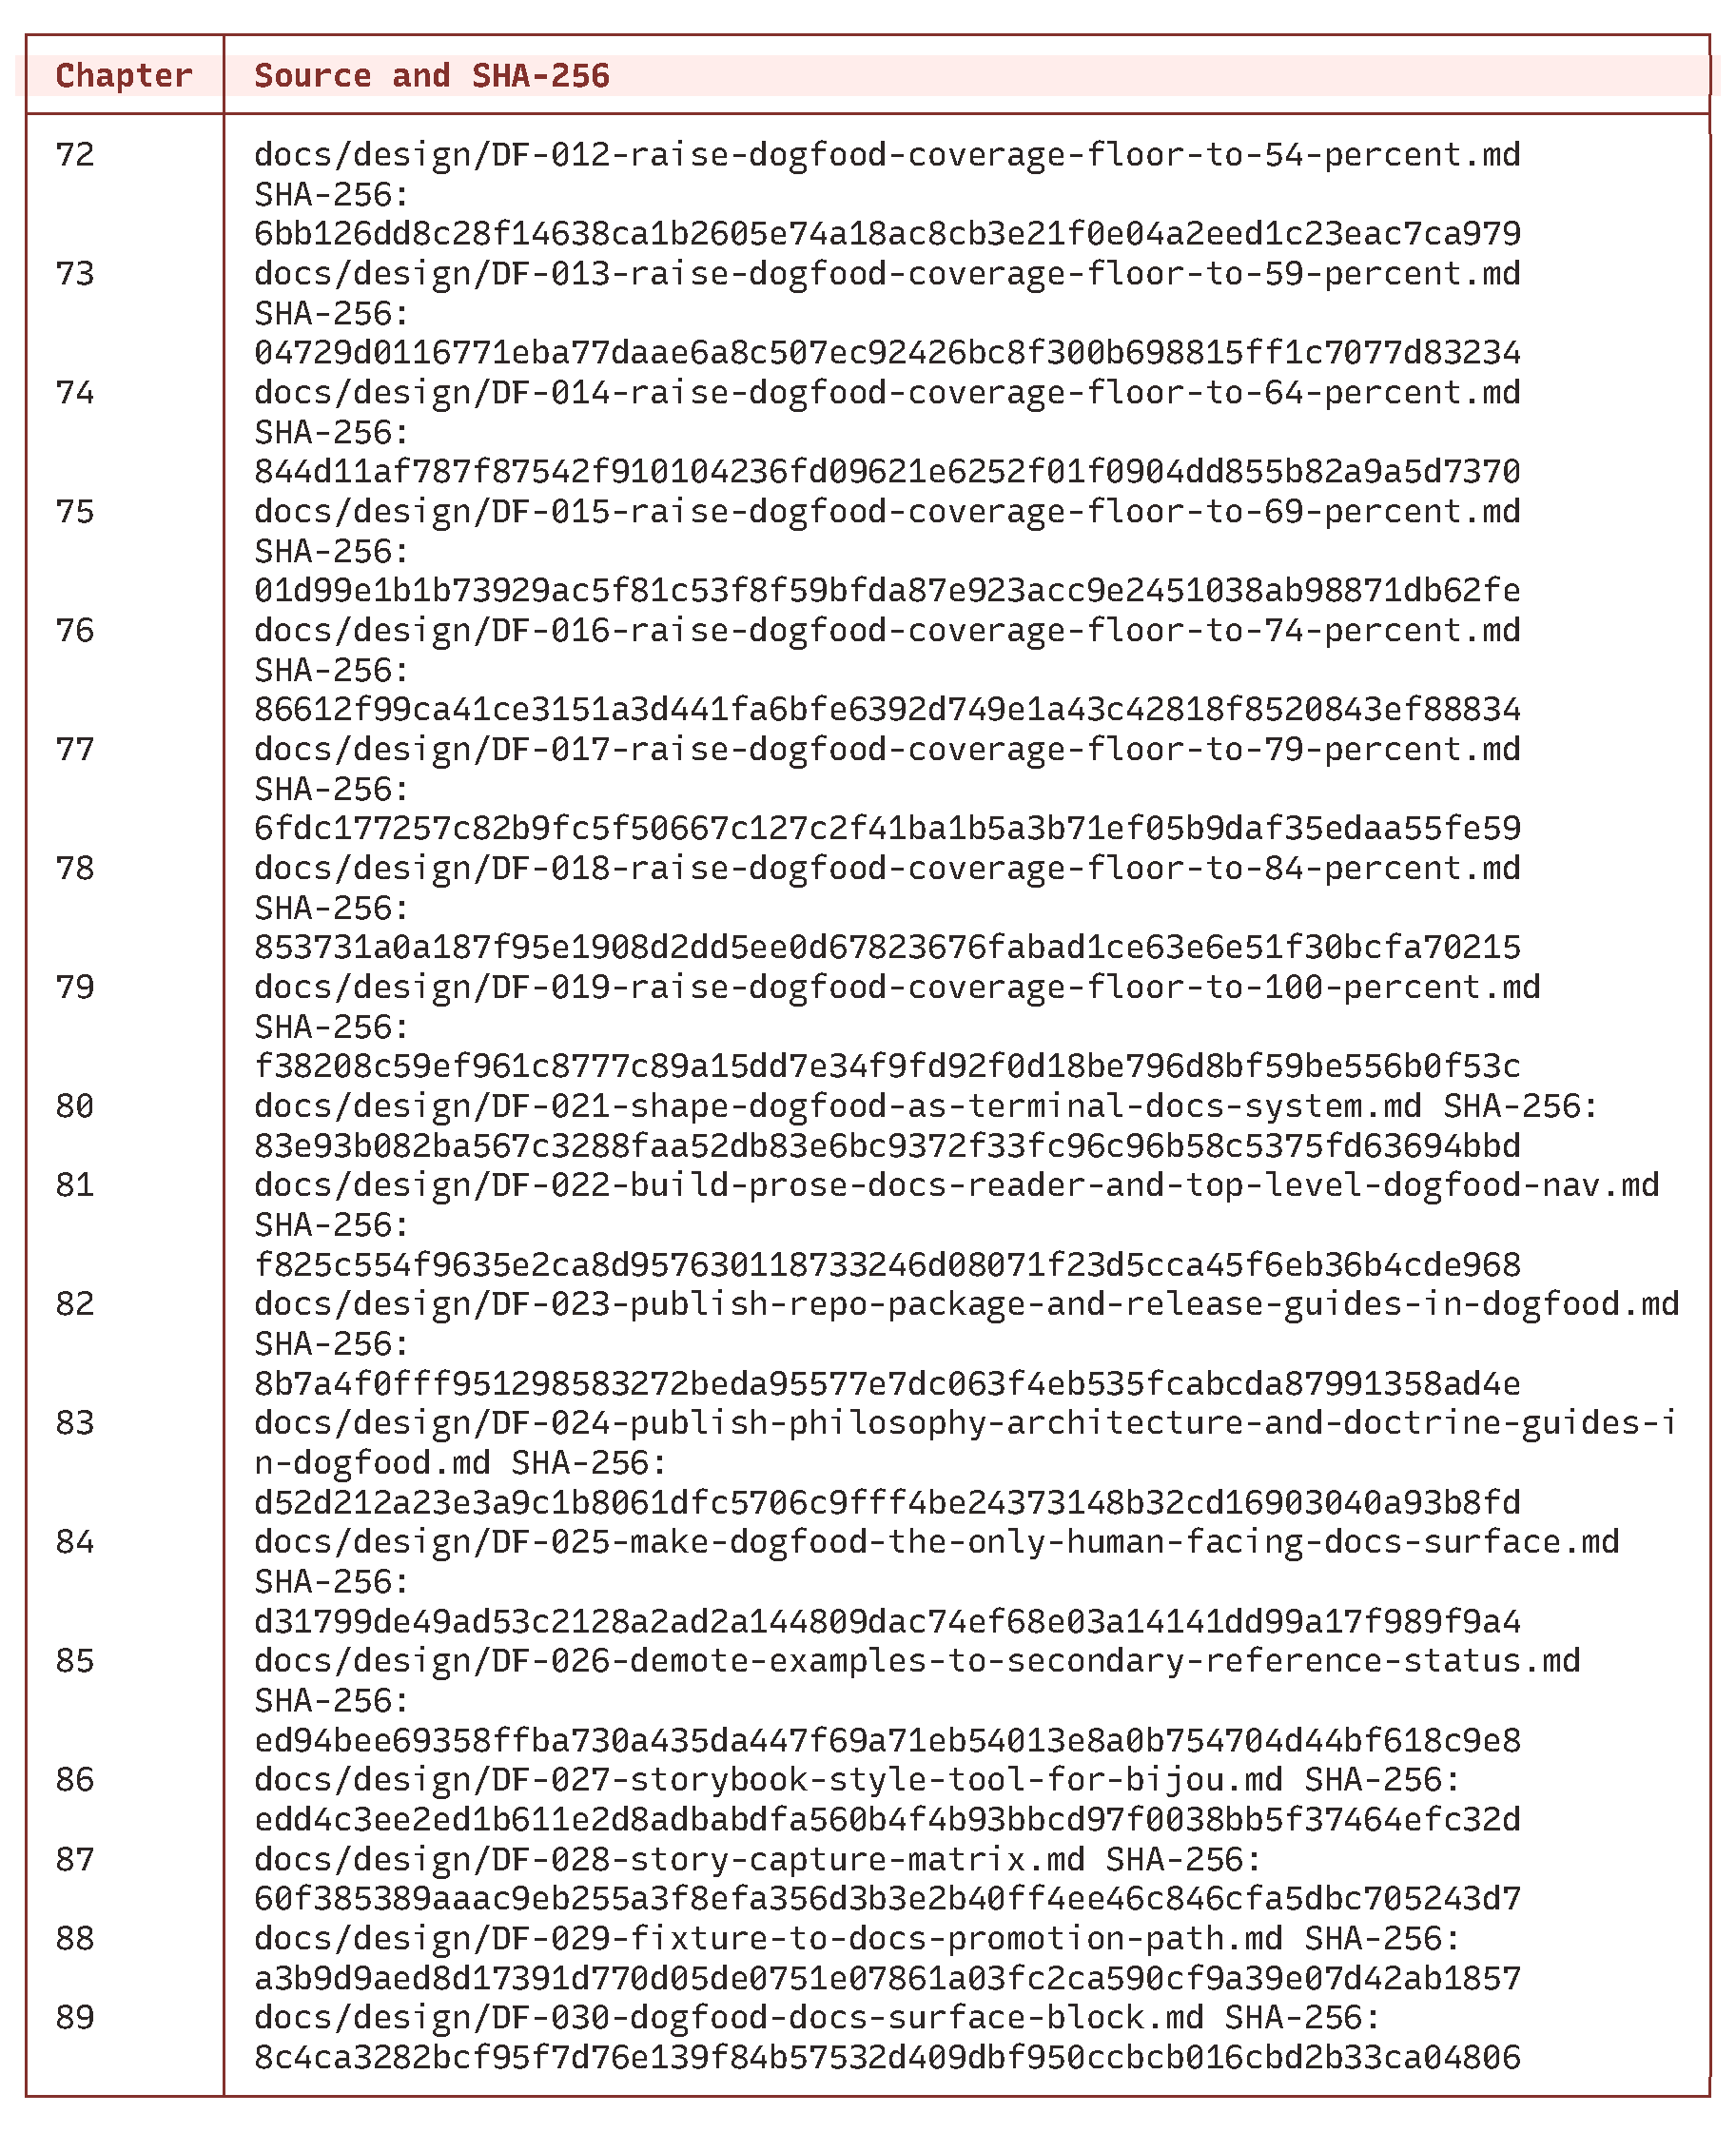
\includegraphics[width=\linewidth]{figures/tables/source-inventory-g1-4.pdf}
\par\smallskip{\scriptsize\color{BookMuted}Rows 72–89. Actual Bijou table component.}
\end{center}
\par\medskip
\begin{center}
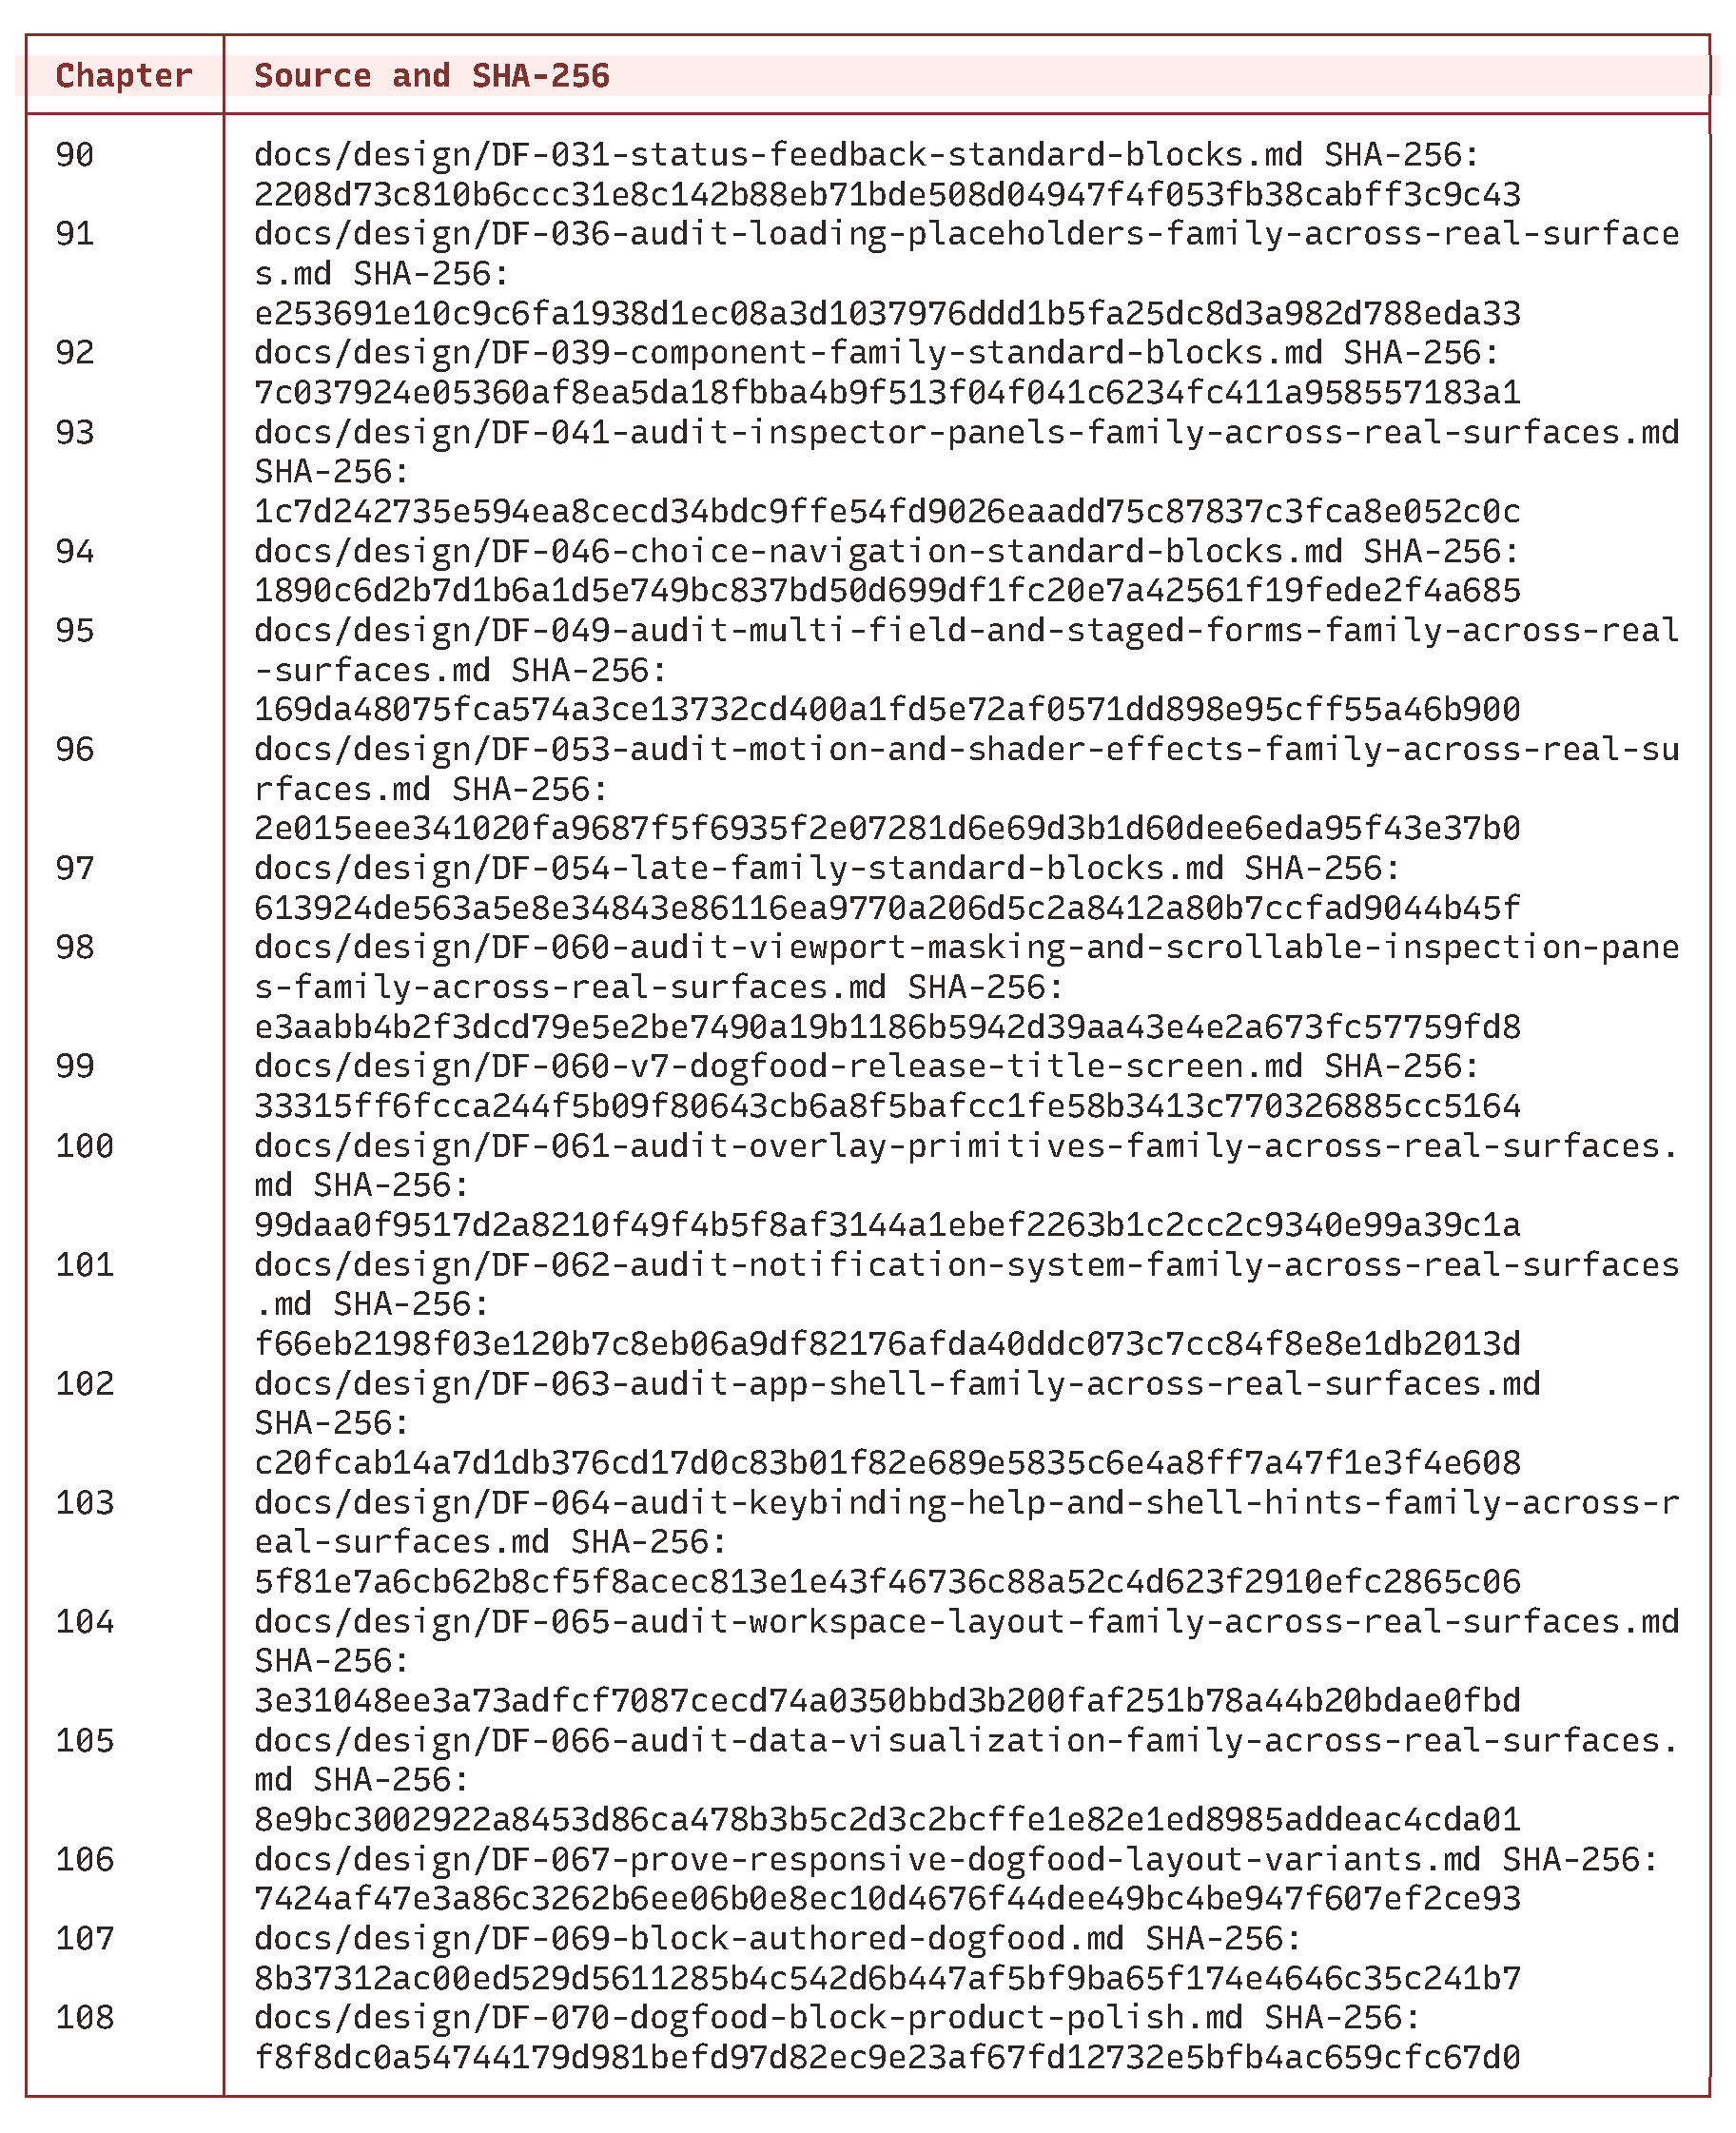
\includegraphics[width=\linewidth]{figures/tables/source-inventory-g1-5.pdf}
\par\smallskip{\scriptsize\color{BookMuted}Rows 90–108. Actual Bijou table component.}
\end{center}
\par\medskip
\begin{center}
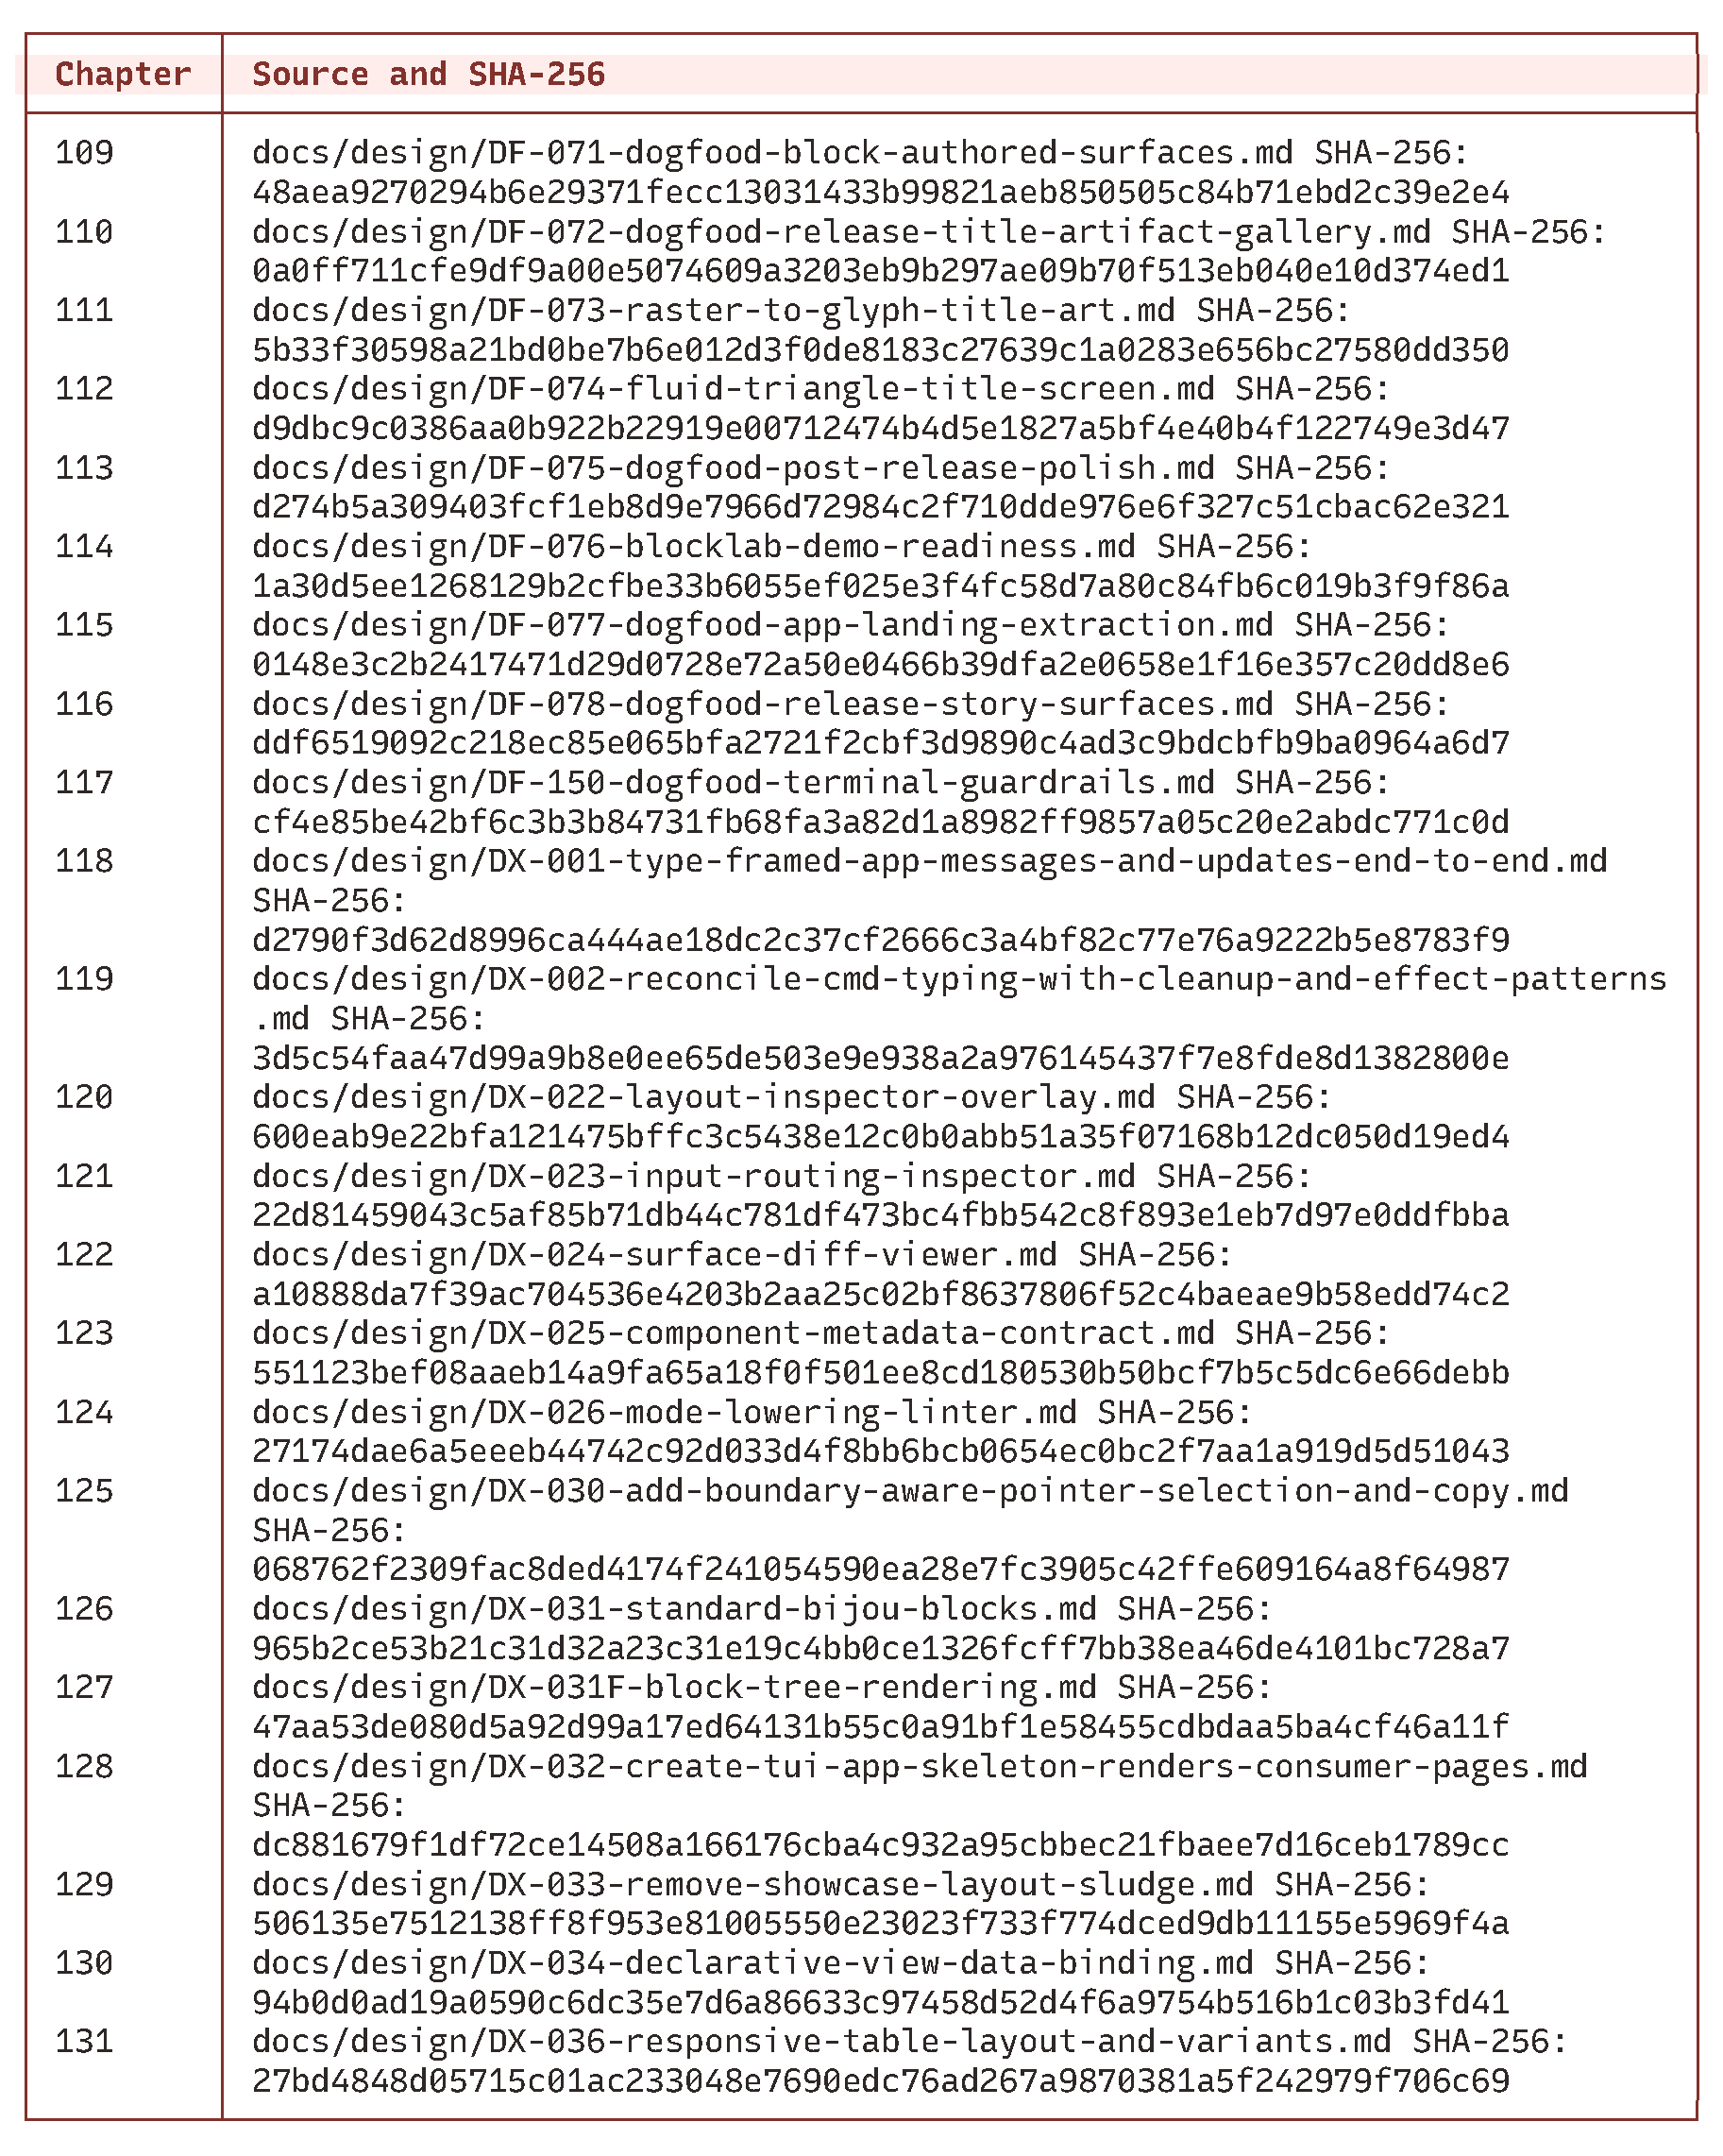
\includegraphics[width=\linewidth]{figures/tables/source-inventory-g1-6.pdf}
\par\smallskip{\scriptsize\color{BookMuted}Rows 109–131. Actual Bijou table component.}
\end{center}
\par\medskip
\begin{center}
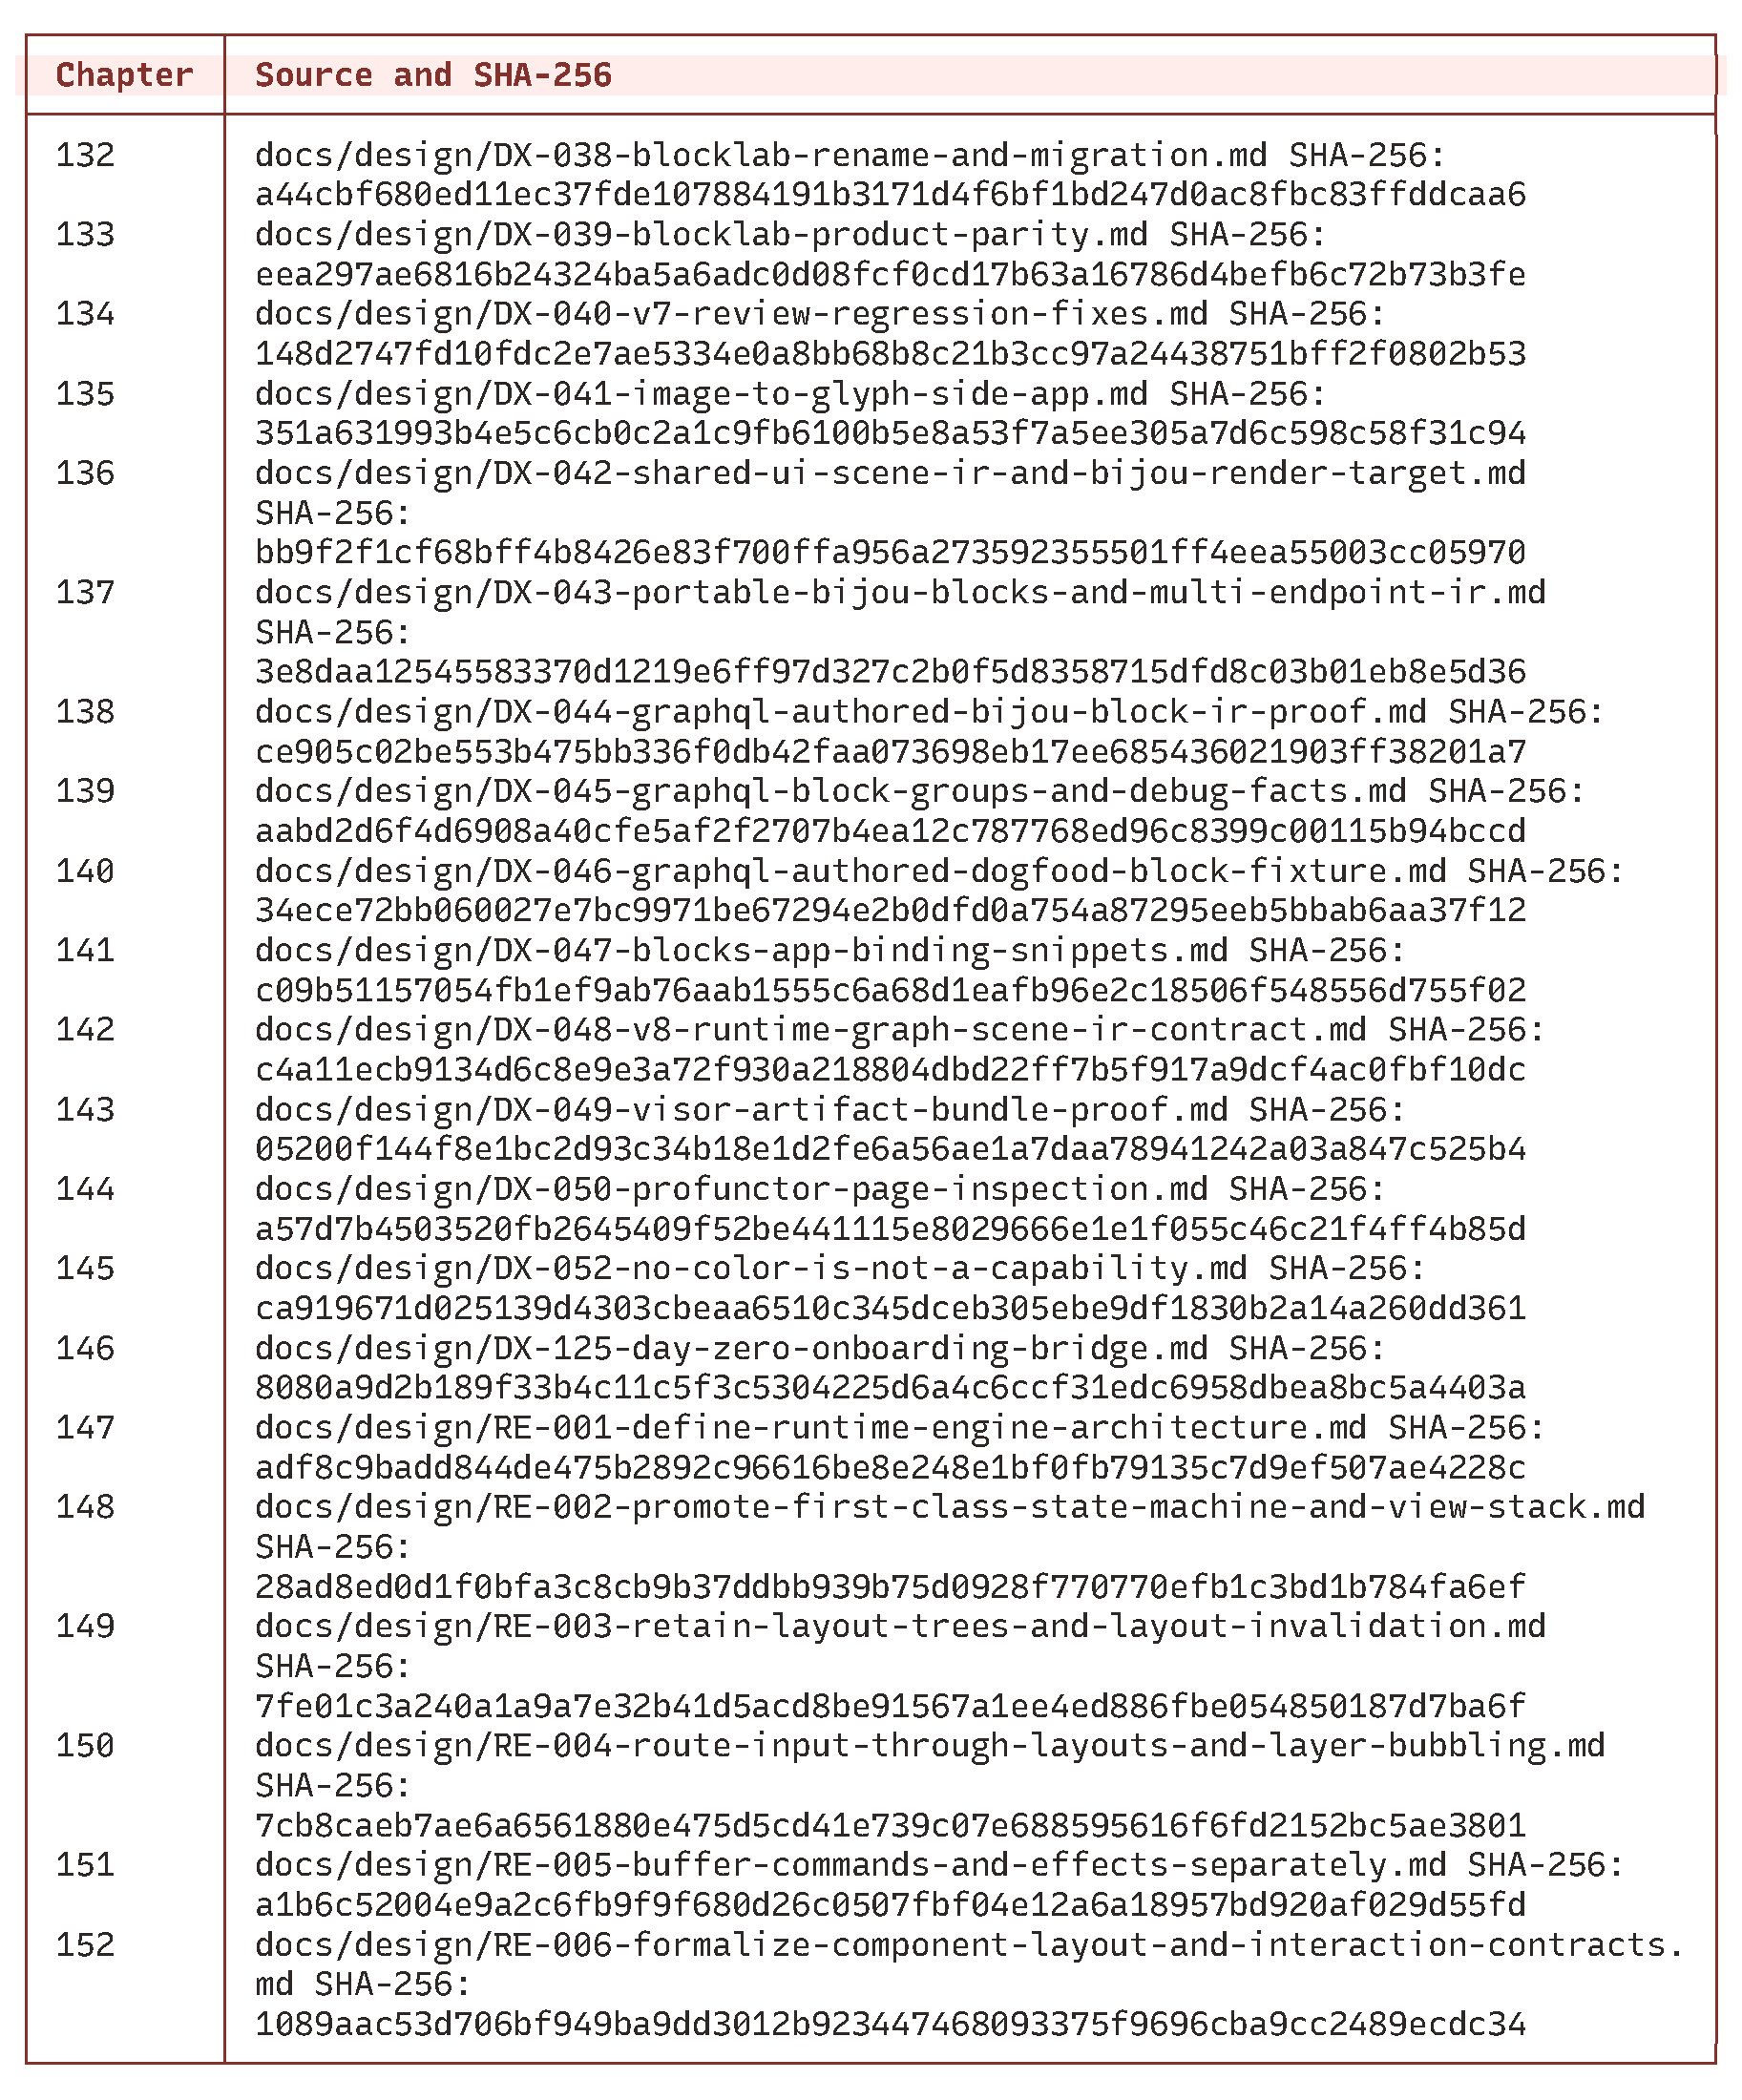
\includegraphics[width=\linewidth]{figures/tables/source-inventory-g1-7.pdf}
\par\smallskip{\scriptsize\color{BookMuted}Rows 132–152. Actual Bijou table component.}
\end{center}
\par\medskip
\begin{center}
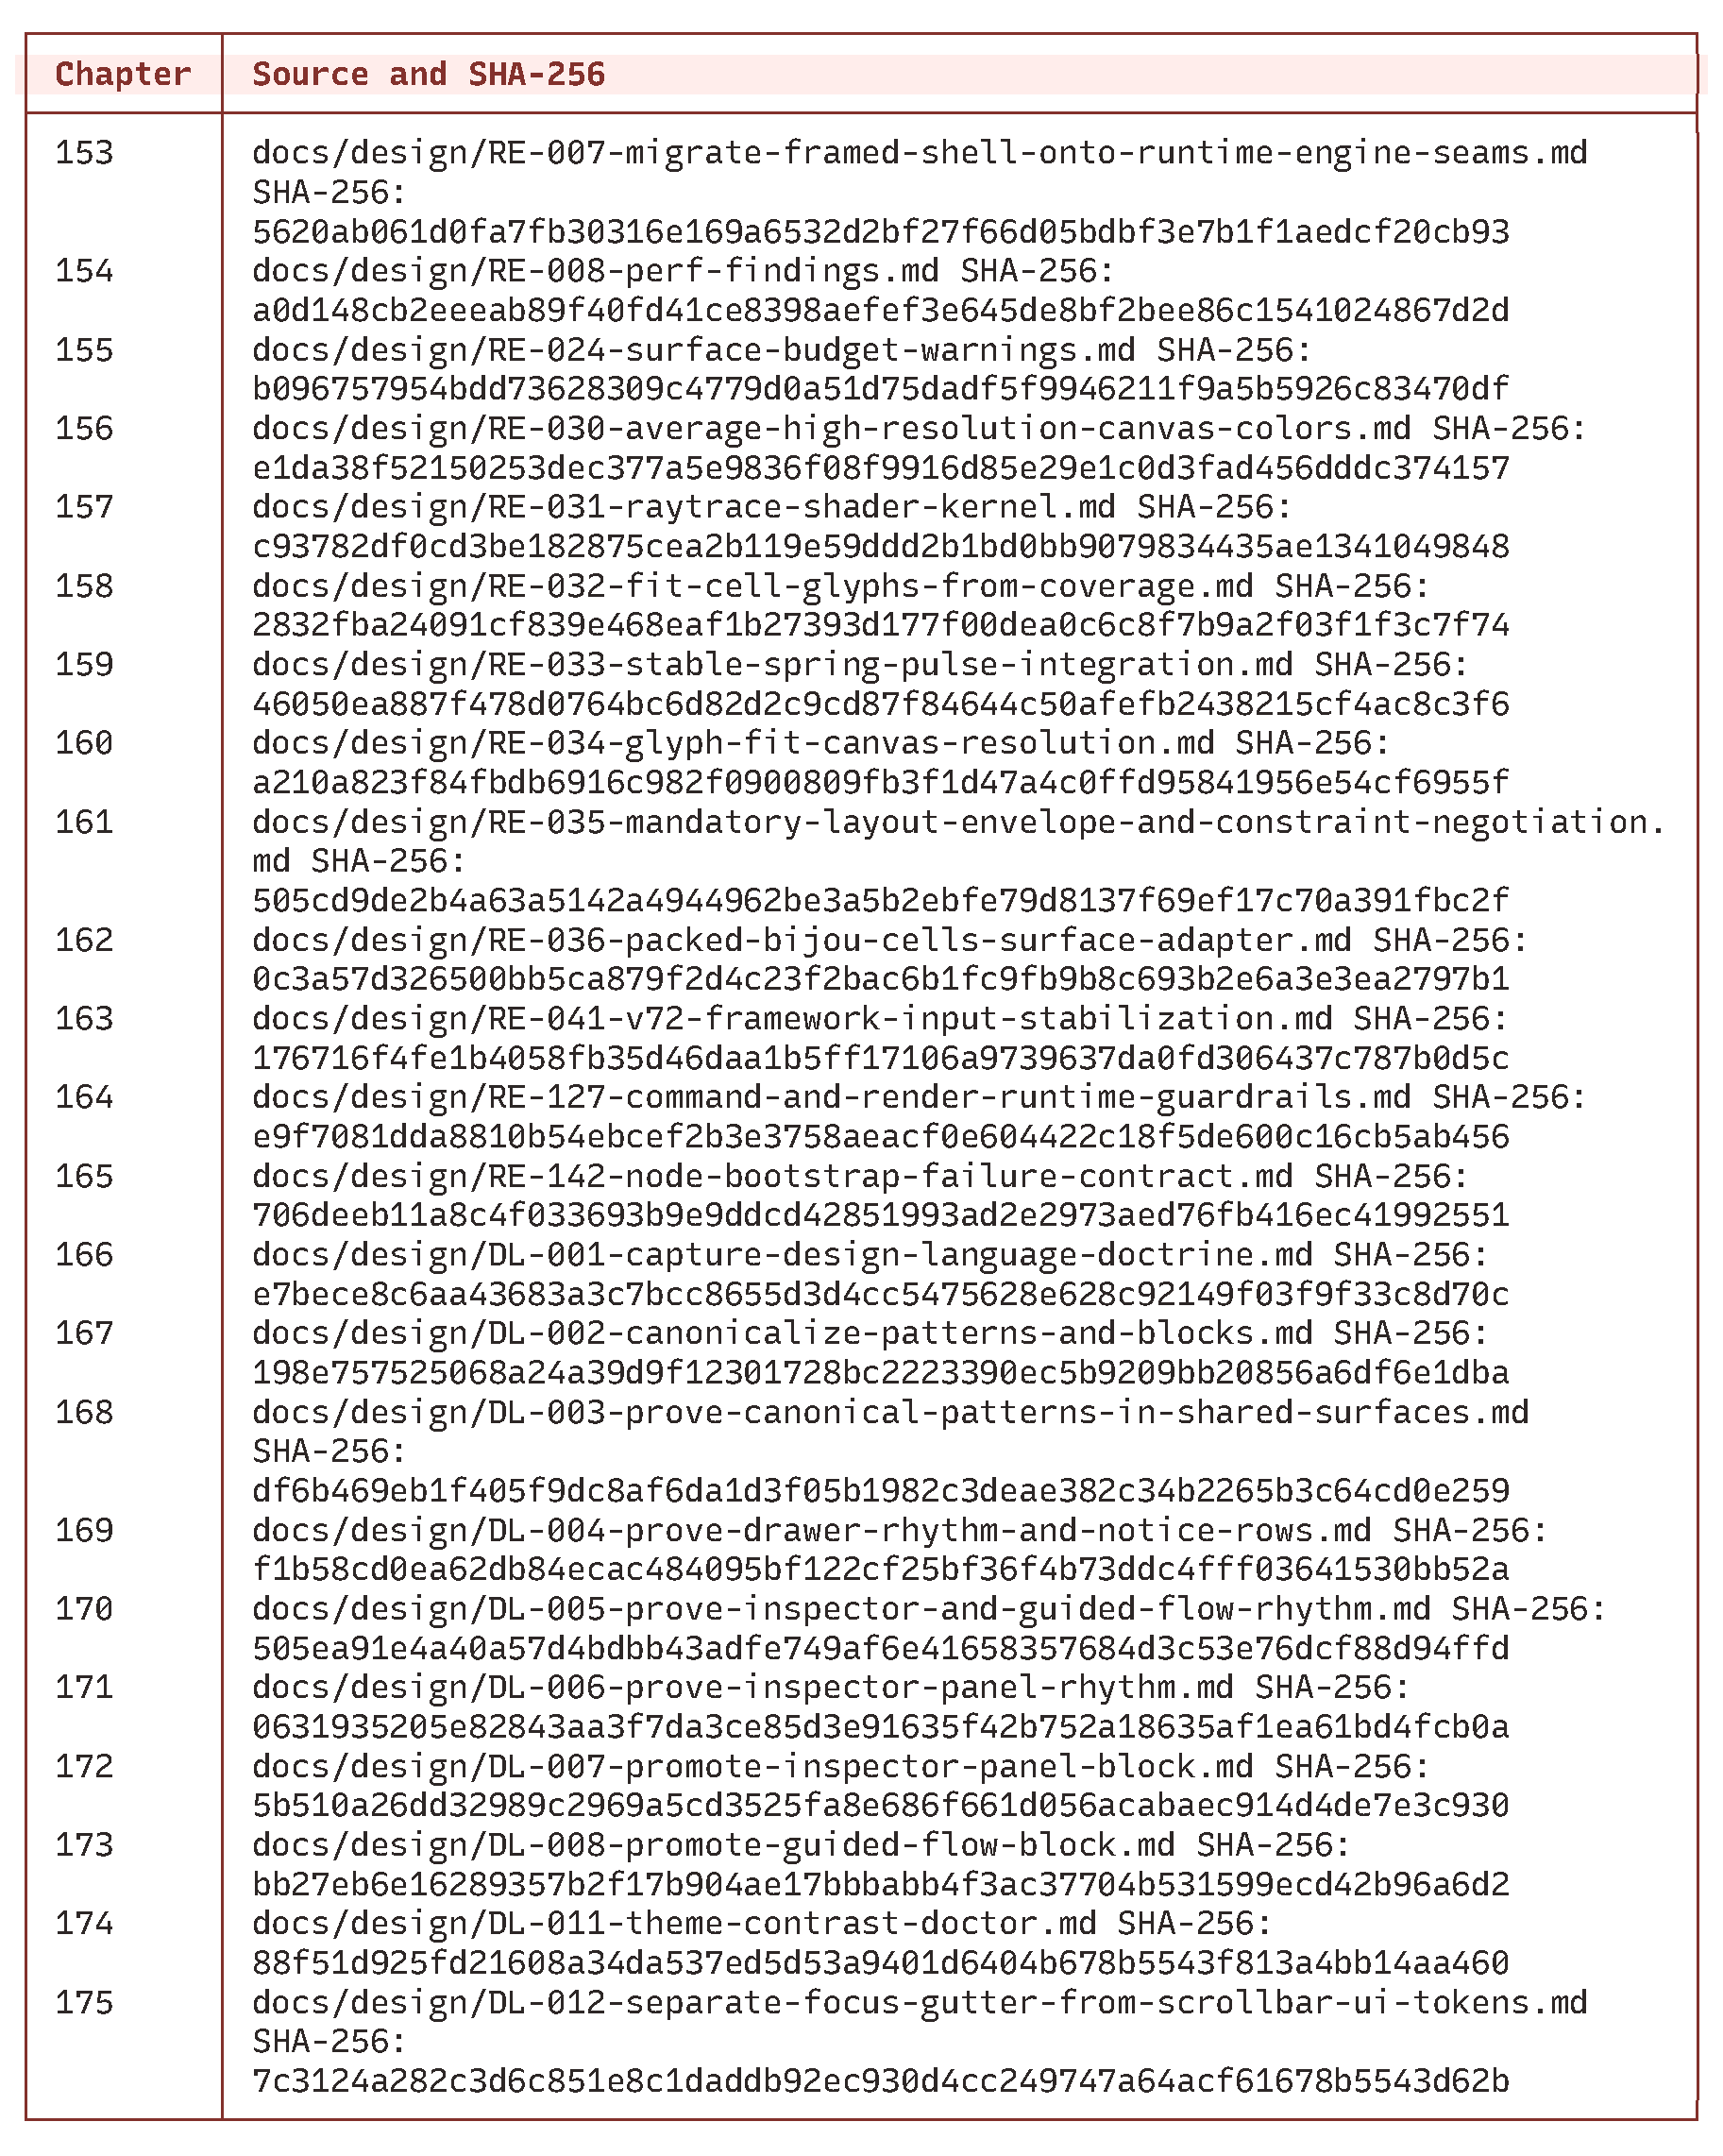
\includegraphics[width=\linewidth]{figures/tables/source-inventory-g1-8.pdf}
\par\smallskip{\scriptsize\color{BookMuted}Rows 153–175. Actual Bijou table component.}
\end{center}
\par\medskip
\begin{center}
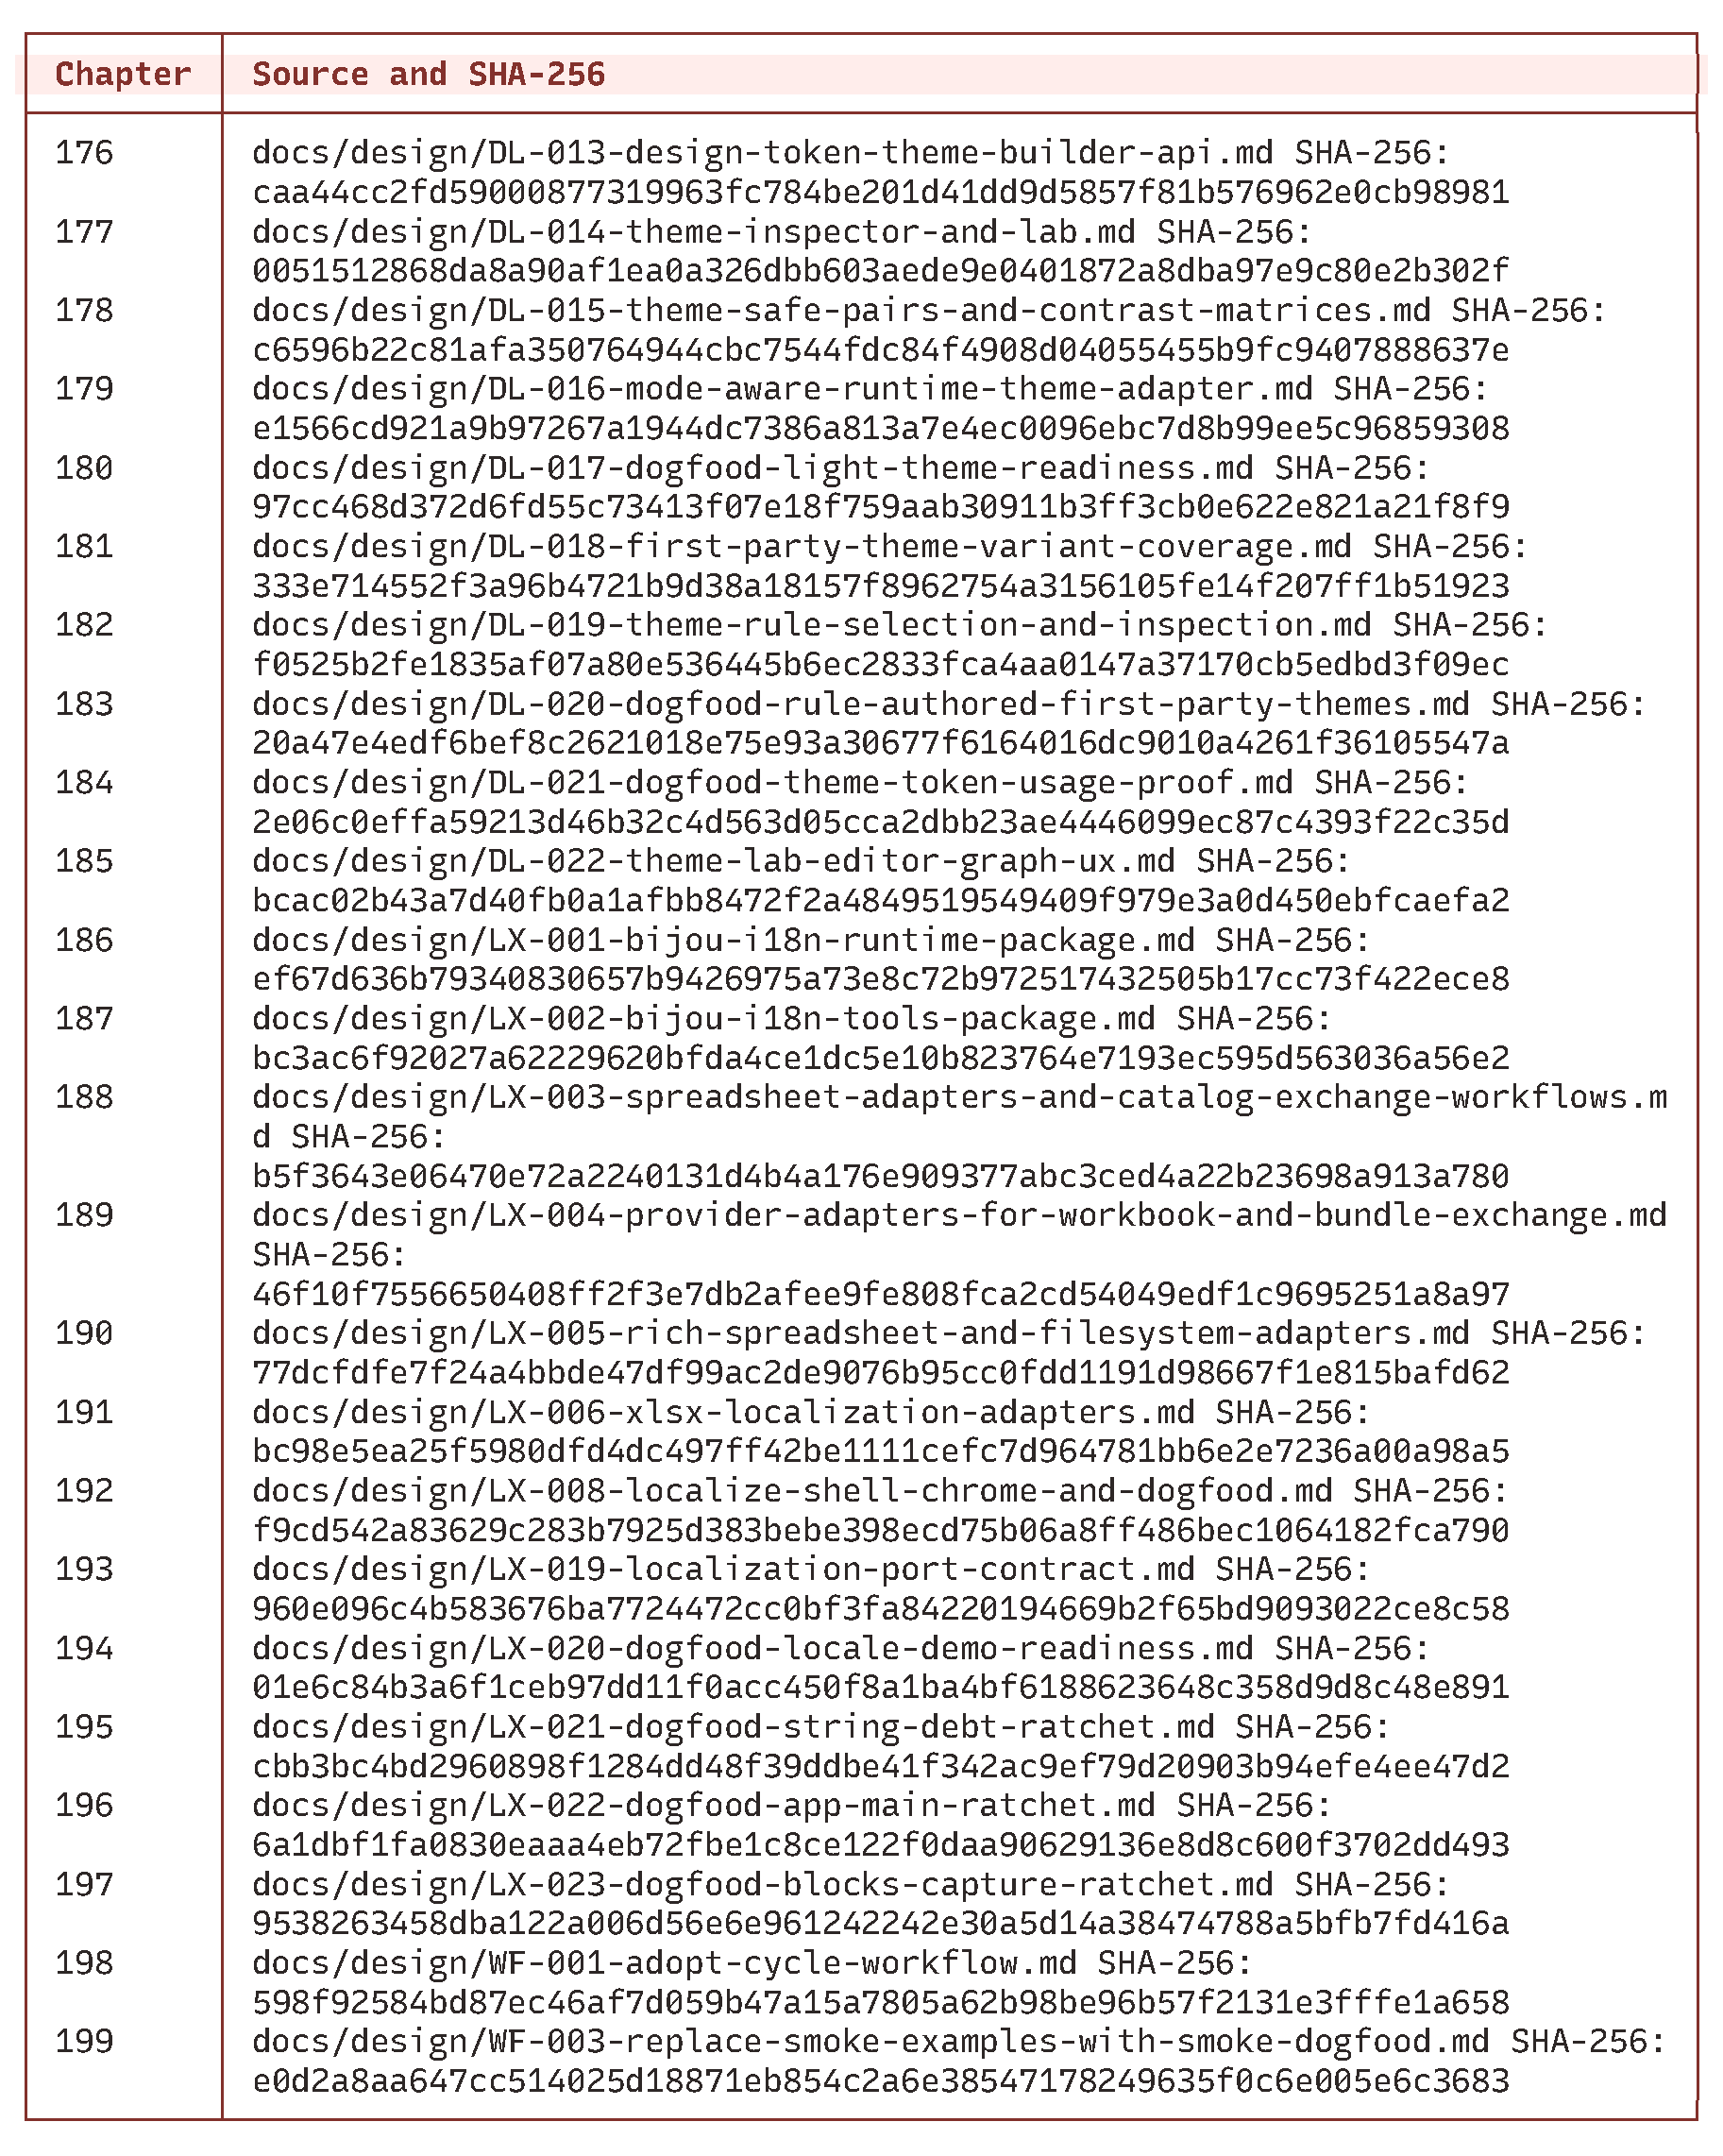
\includegraphics[width=\linewidth]{figures/tables/source-inventory-g1-9.pdf}
\par\smallskip{\scriptsize\color{BookMuted}Rows 176–199. Actual Bijou table component.}
\end{center}
\par\medskip
\begin{center}
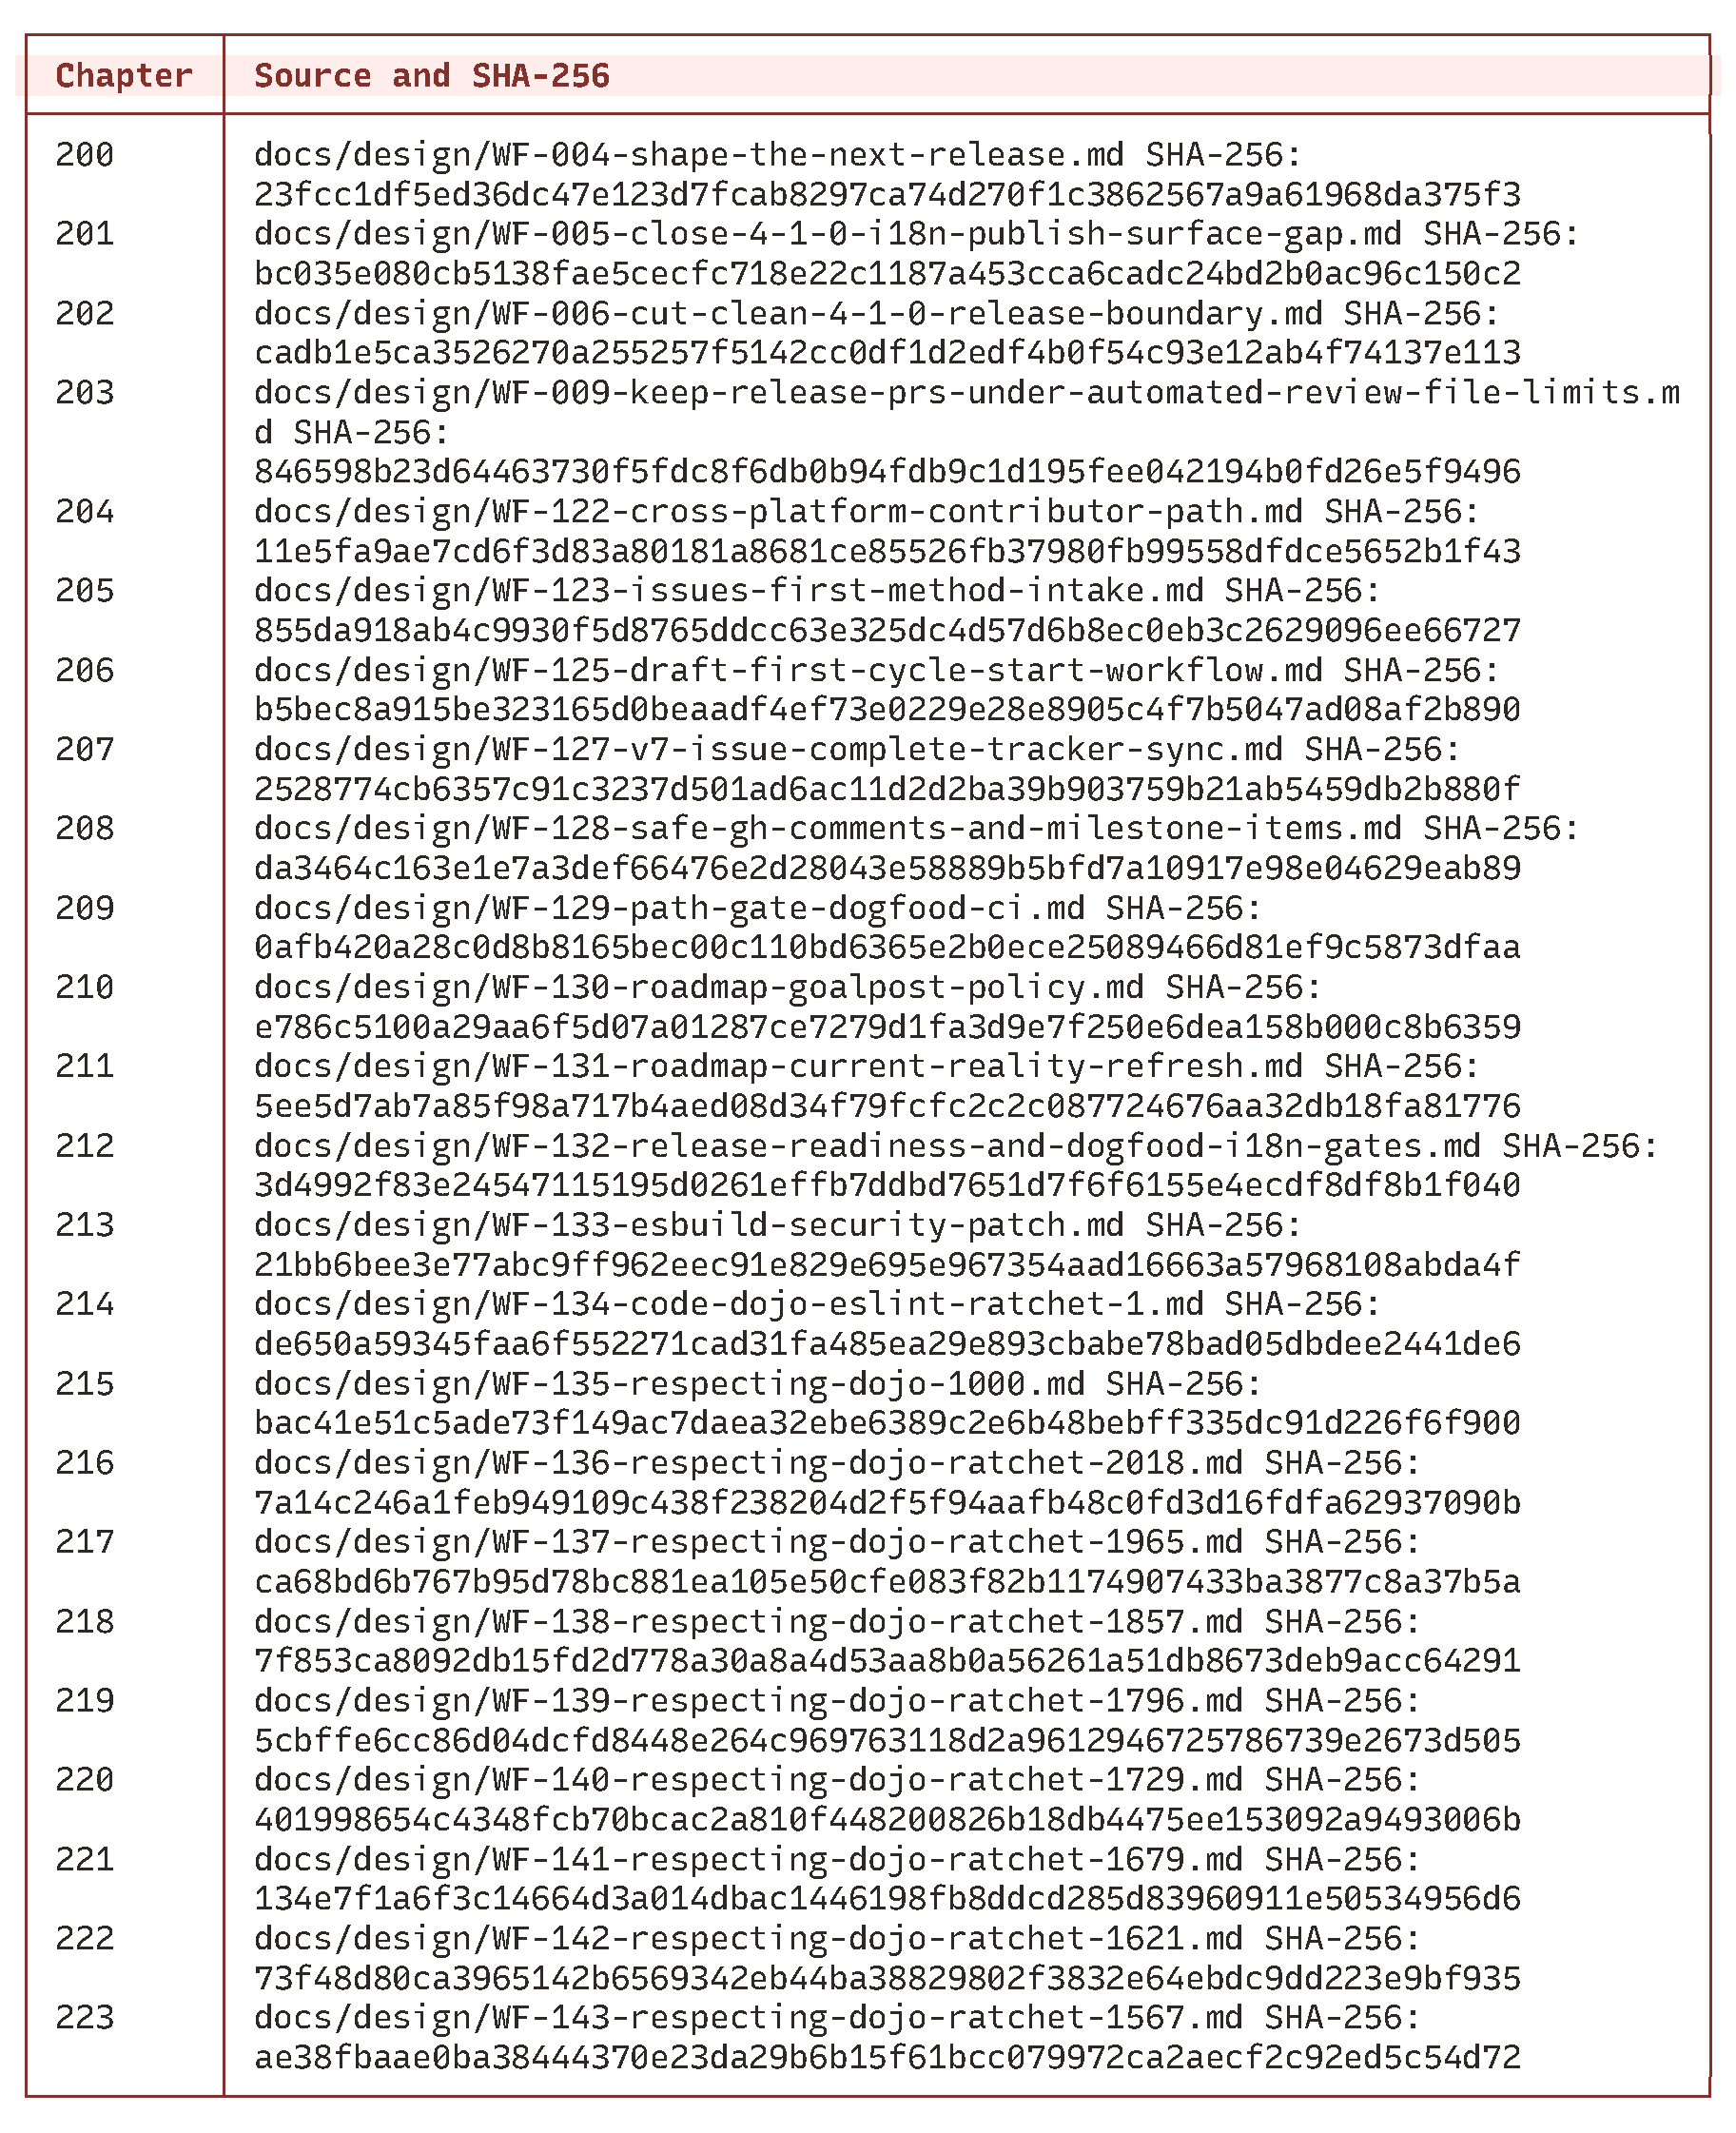
\includegraphics[width=\linewidth]{figures/tables/source-inventory-g1-10.pdf}
\par\smallskip{\scriptsize\color{BookMuted}Rows 200–223. Actual Bijou table component.}
\end{center}
\par\medskip
\begin{center}
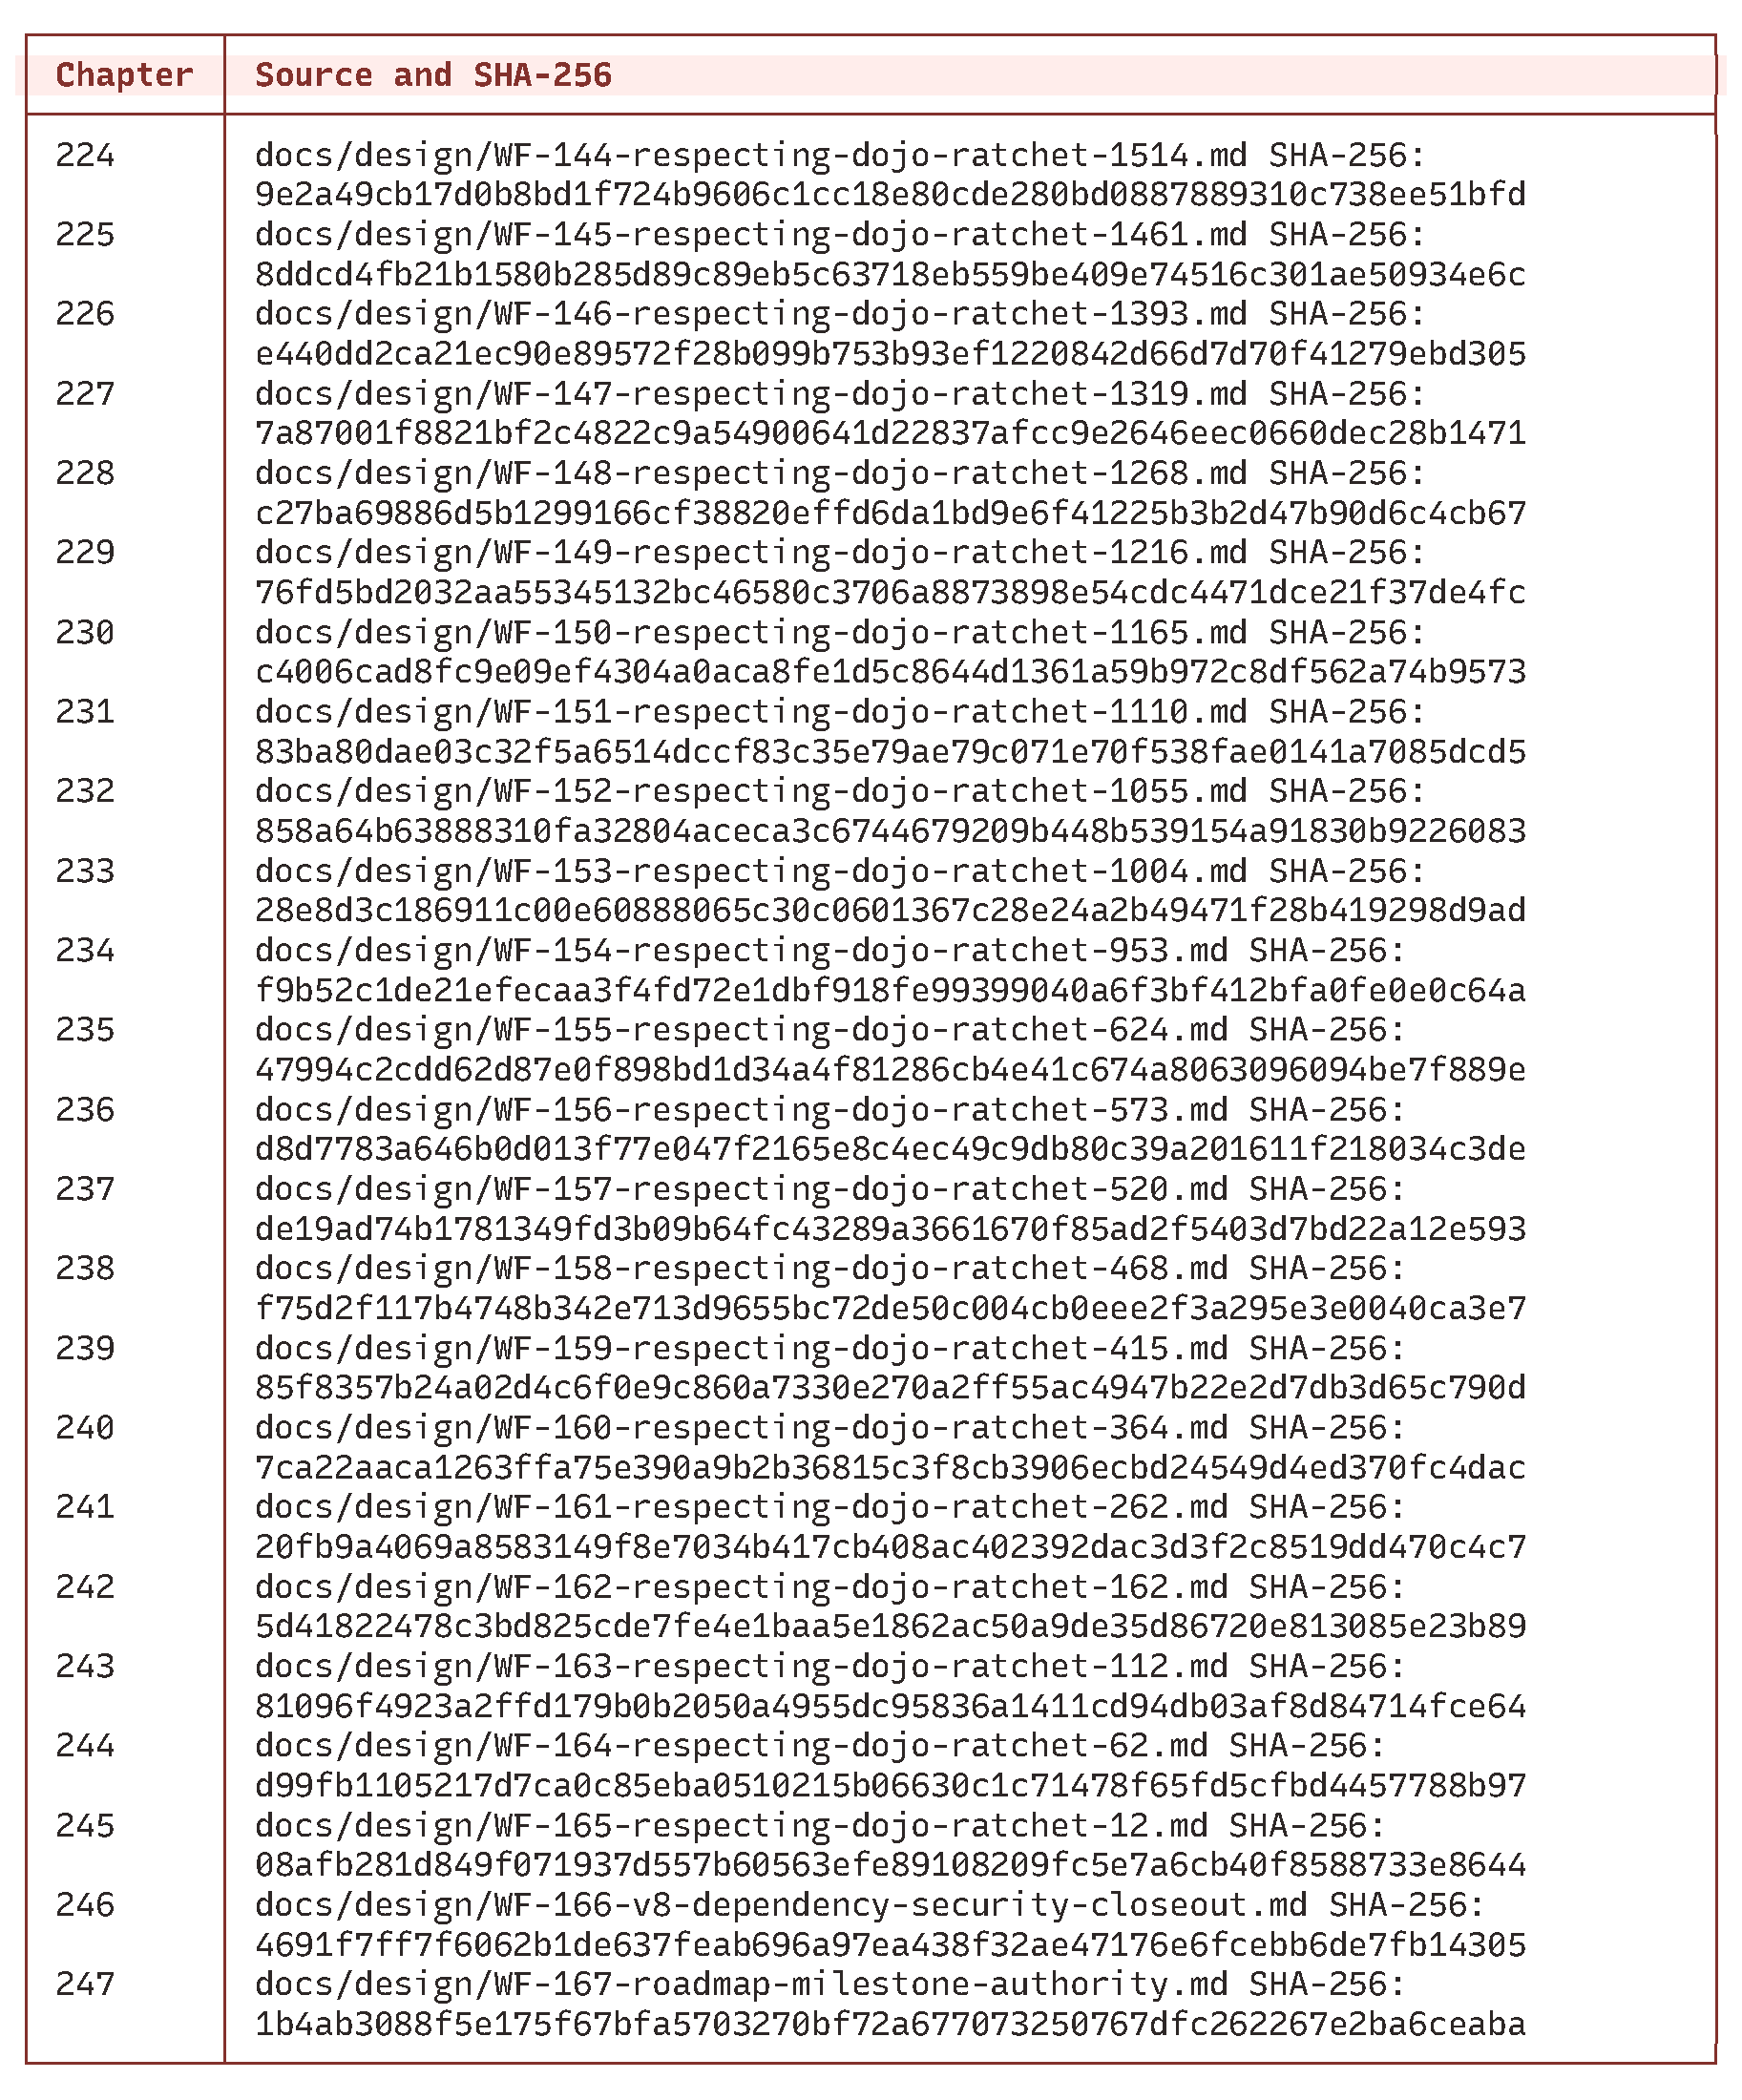
\includegraphics[width=\linewidth]{figures/tables/source-inventory-g1-11.pdf}
\par\smallskip{\scriptsize\color{BookMuted}Rows 224–247. Actual Bijou table component.}
\end{center}
\par\medskip
\begin{center}
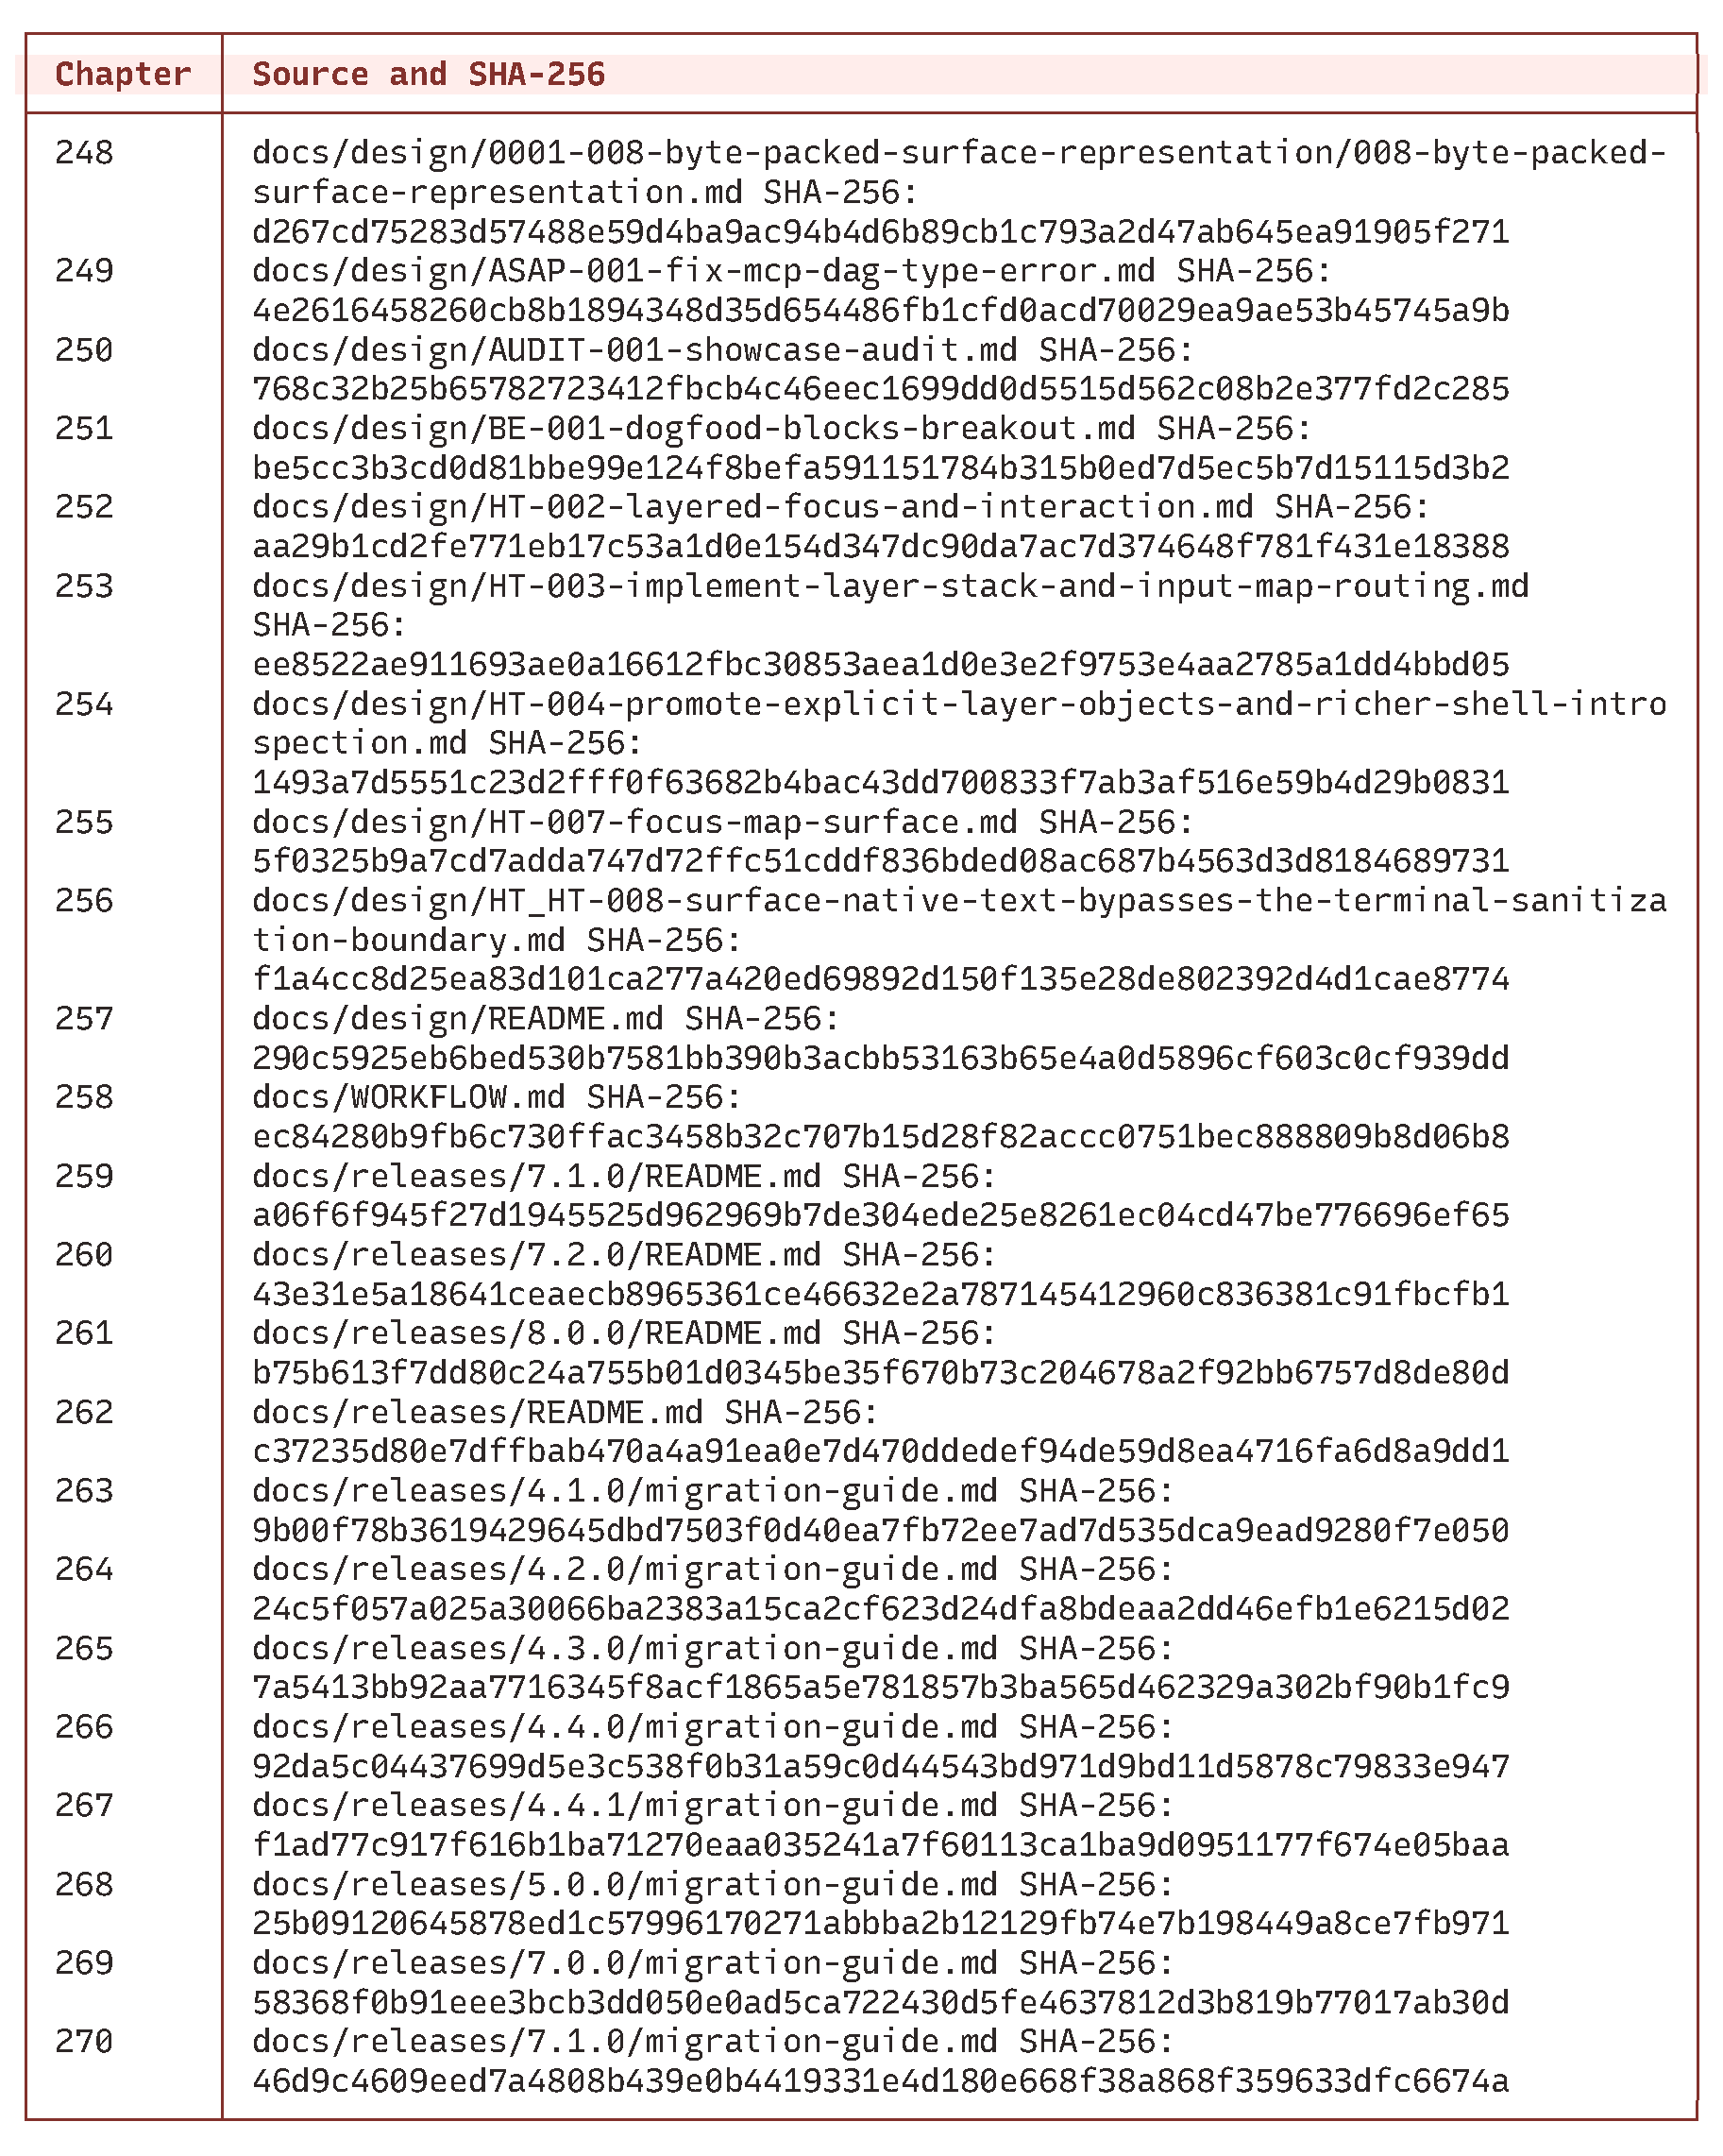
\includegraphics[width=\linewidth]{figures/tables/source-inventory-g1-12.pdf}
\par\smallskip{\scriptsize\color{BookMuted}Rows 248–270. Actual Bijou table component.}
\end{center}
\par\medskip
\begin{center}
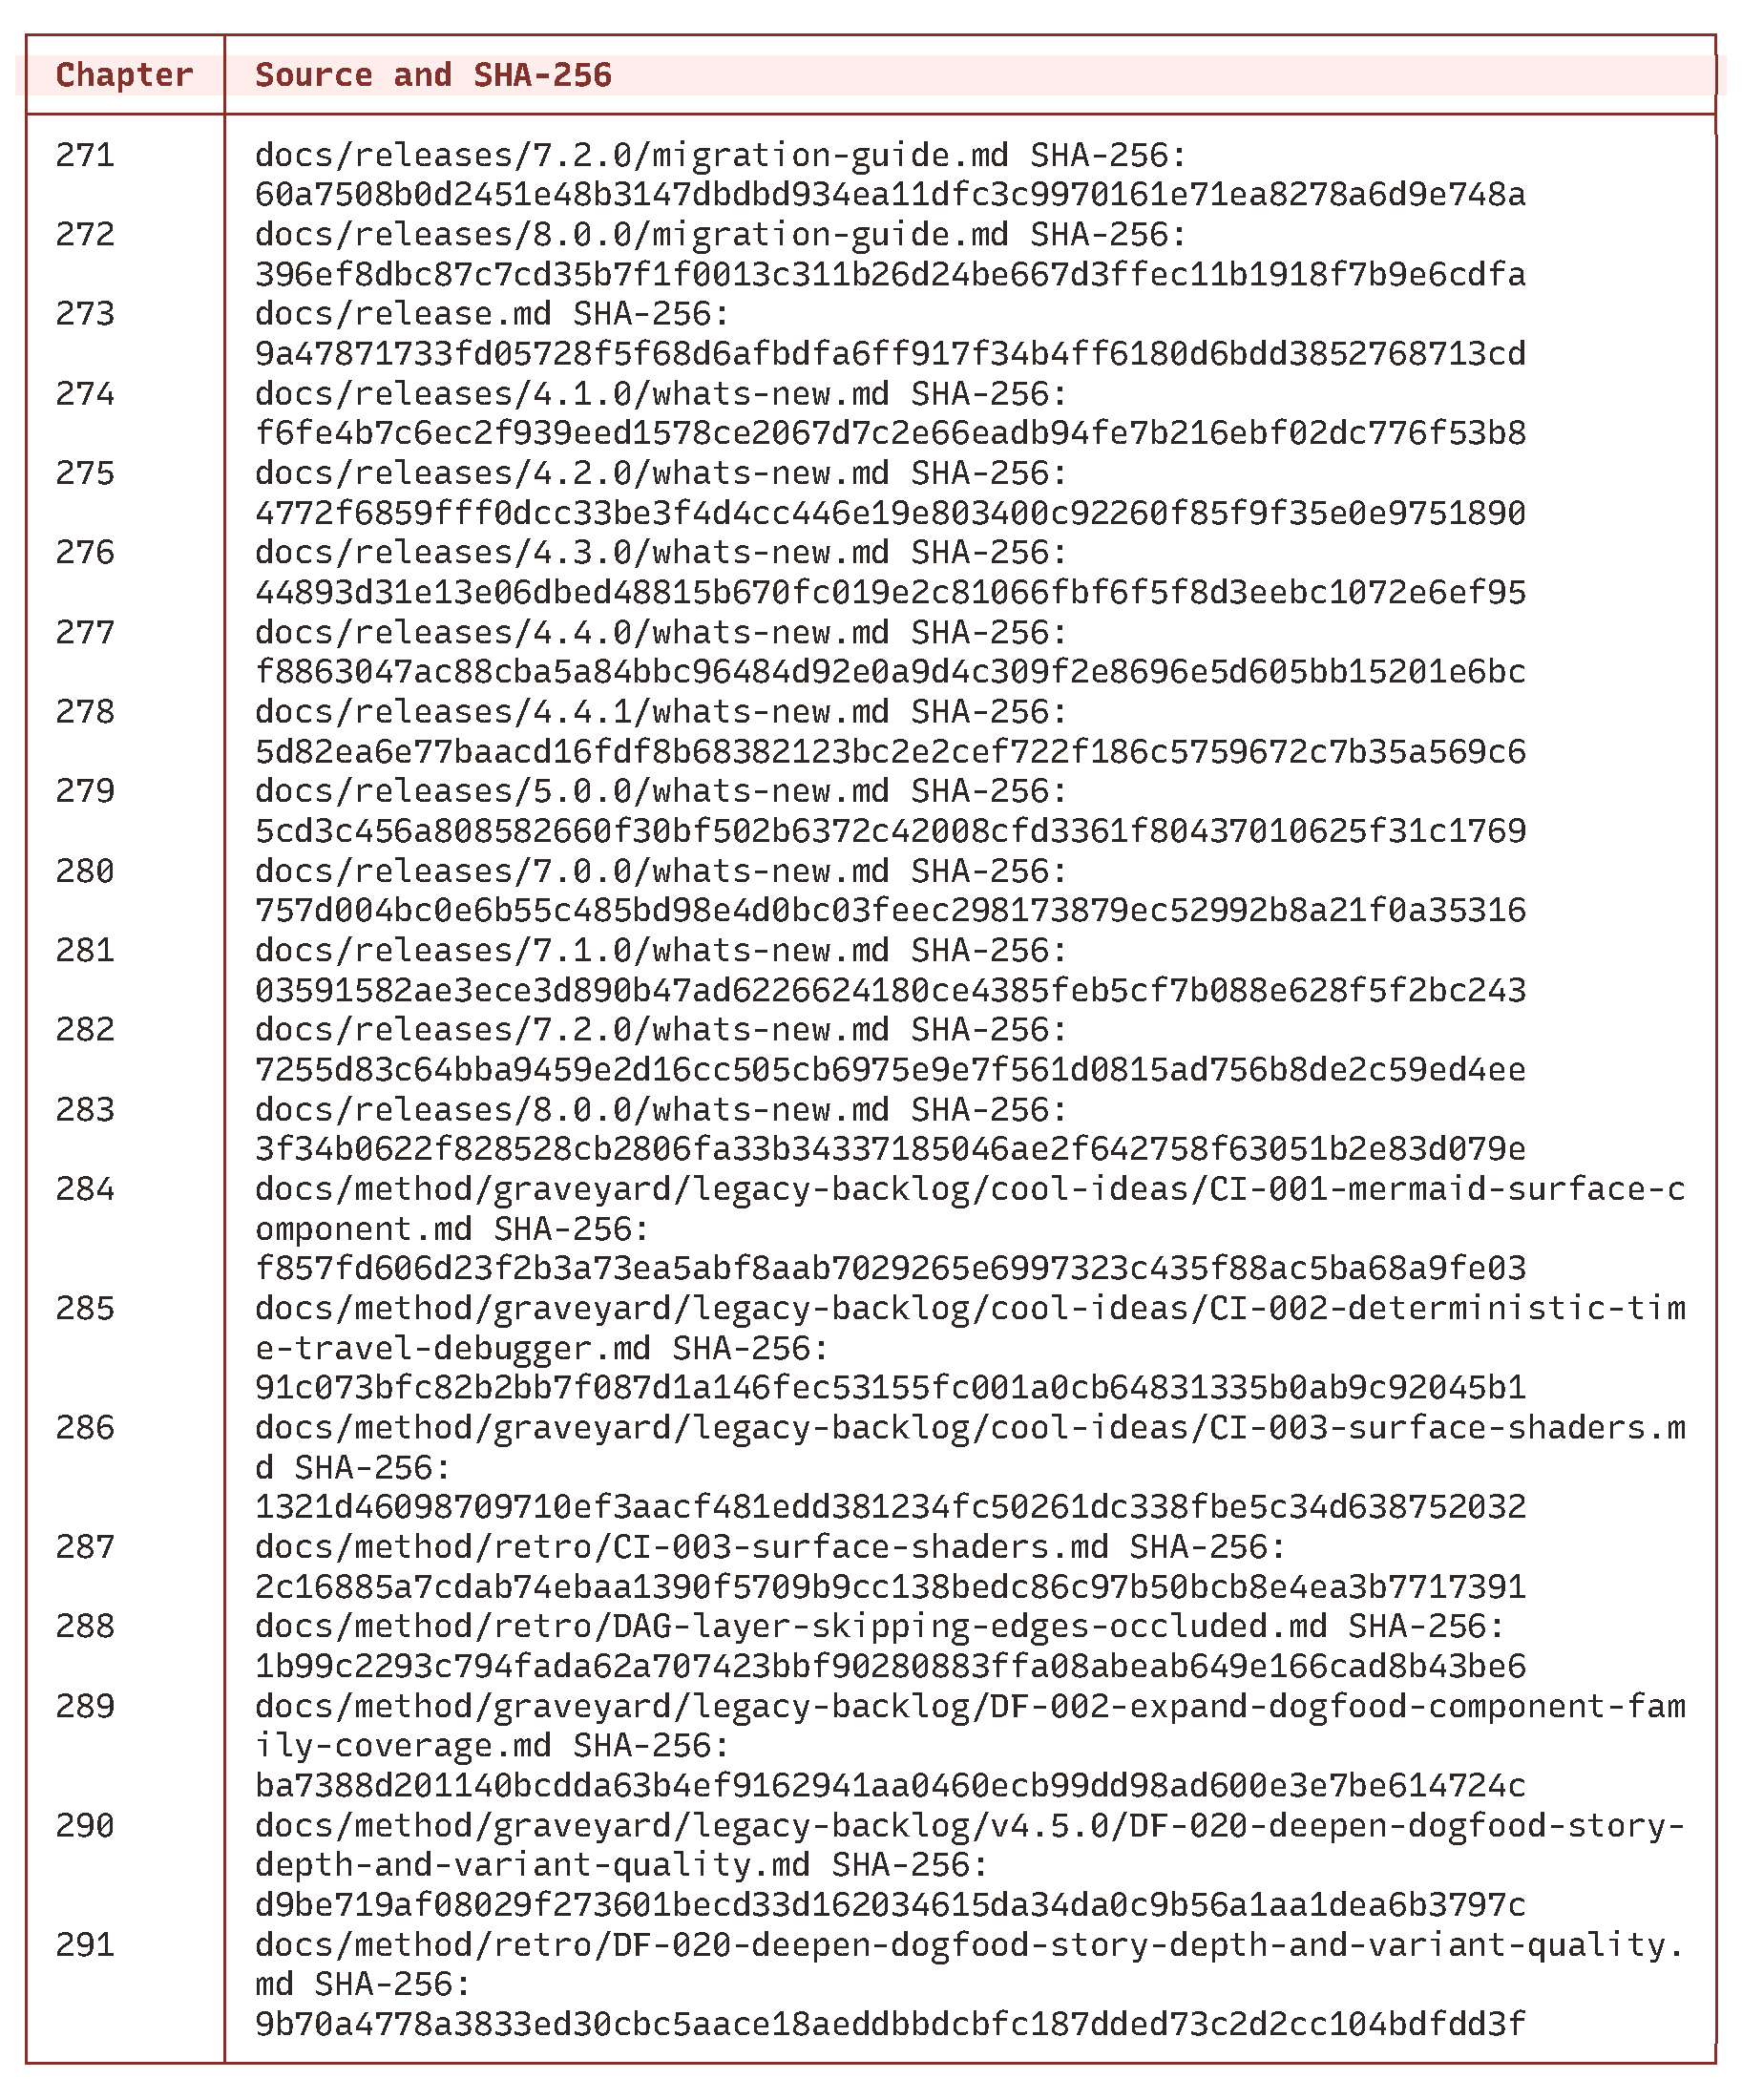
\includegraphics[width=\linewidth]{figures/tables/source-inventory-g1-13.pdf}
\par\smallskip{\scriptsize\color{BookMuted}Rows 271–291. Actual Bijou table component.}
\end{center}
\par\medskip
\begin{center}
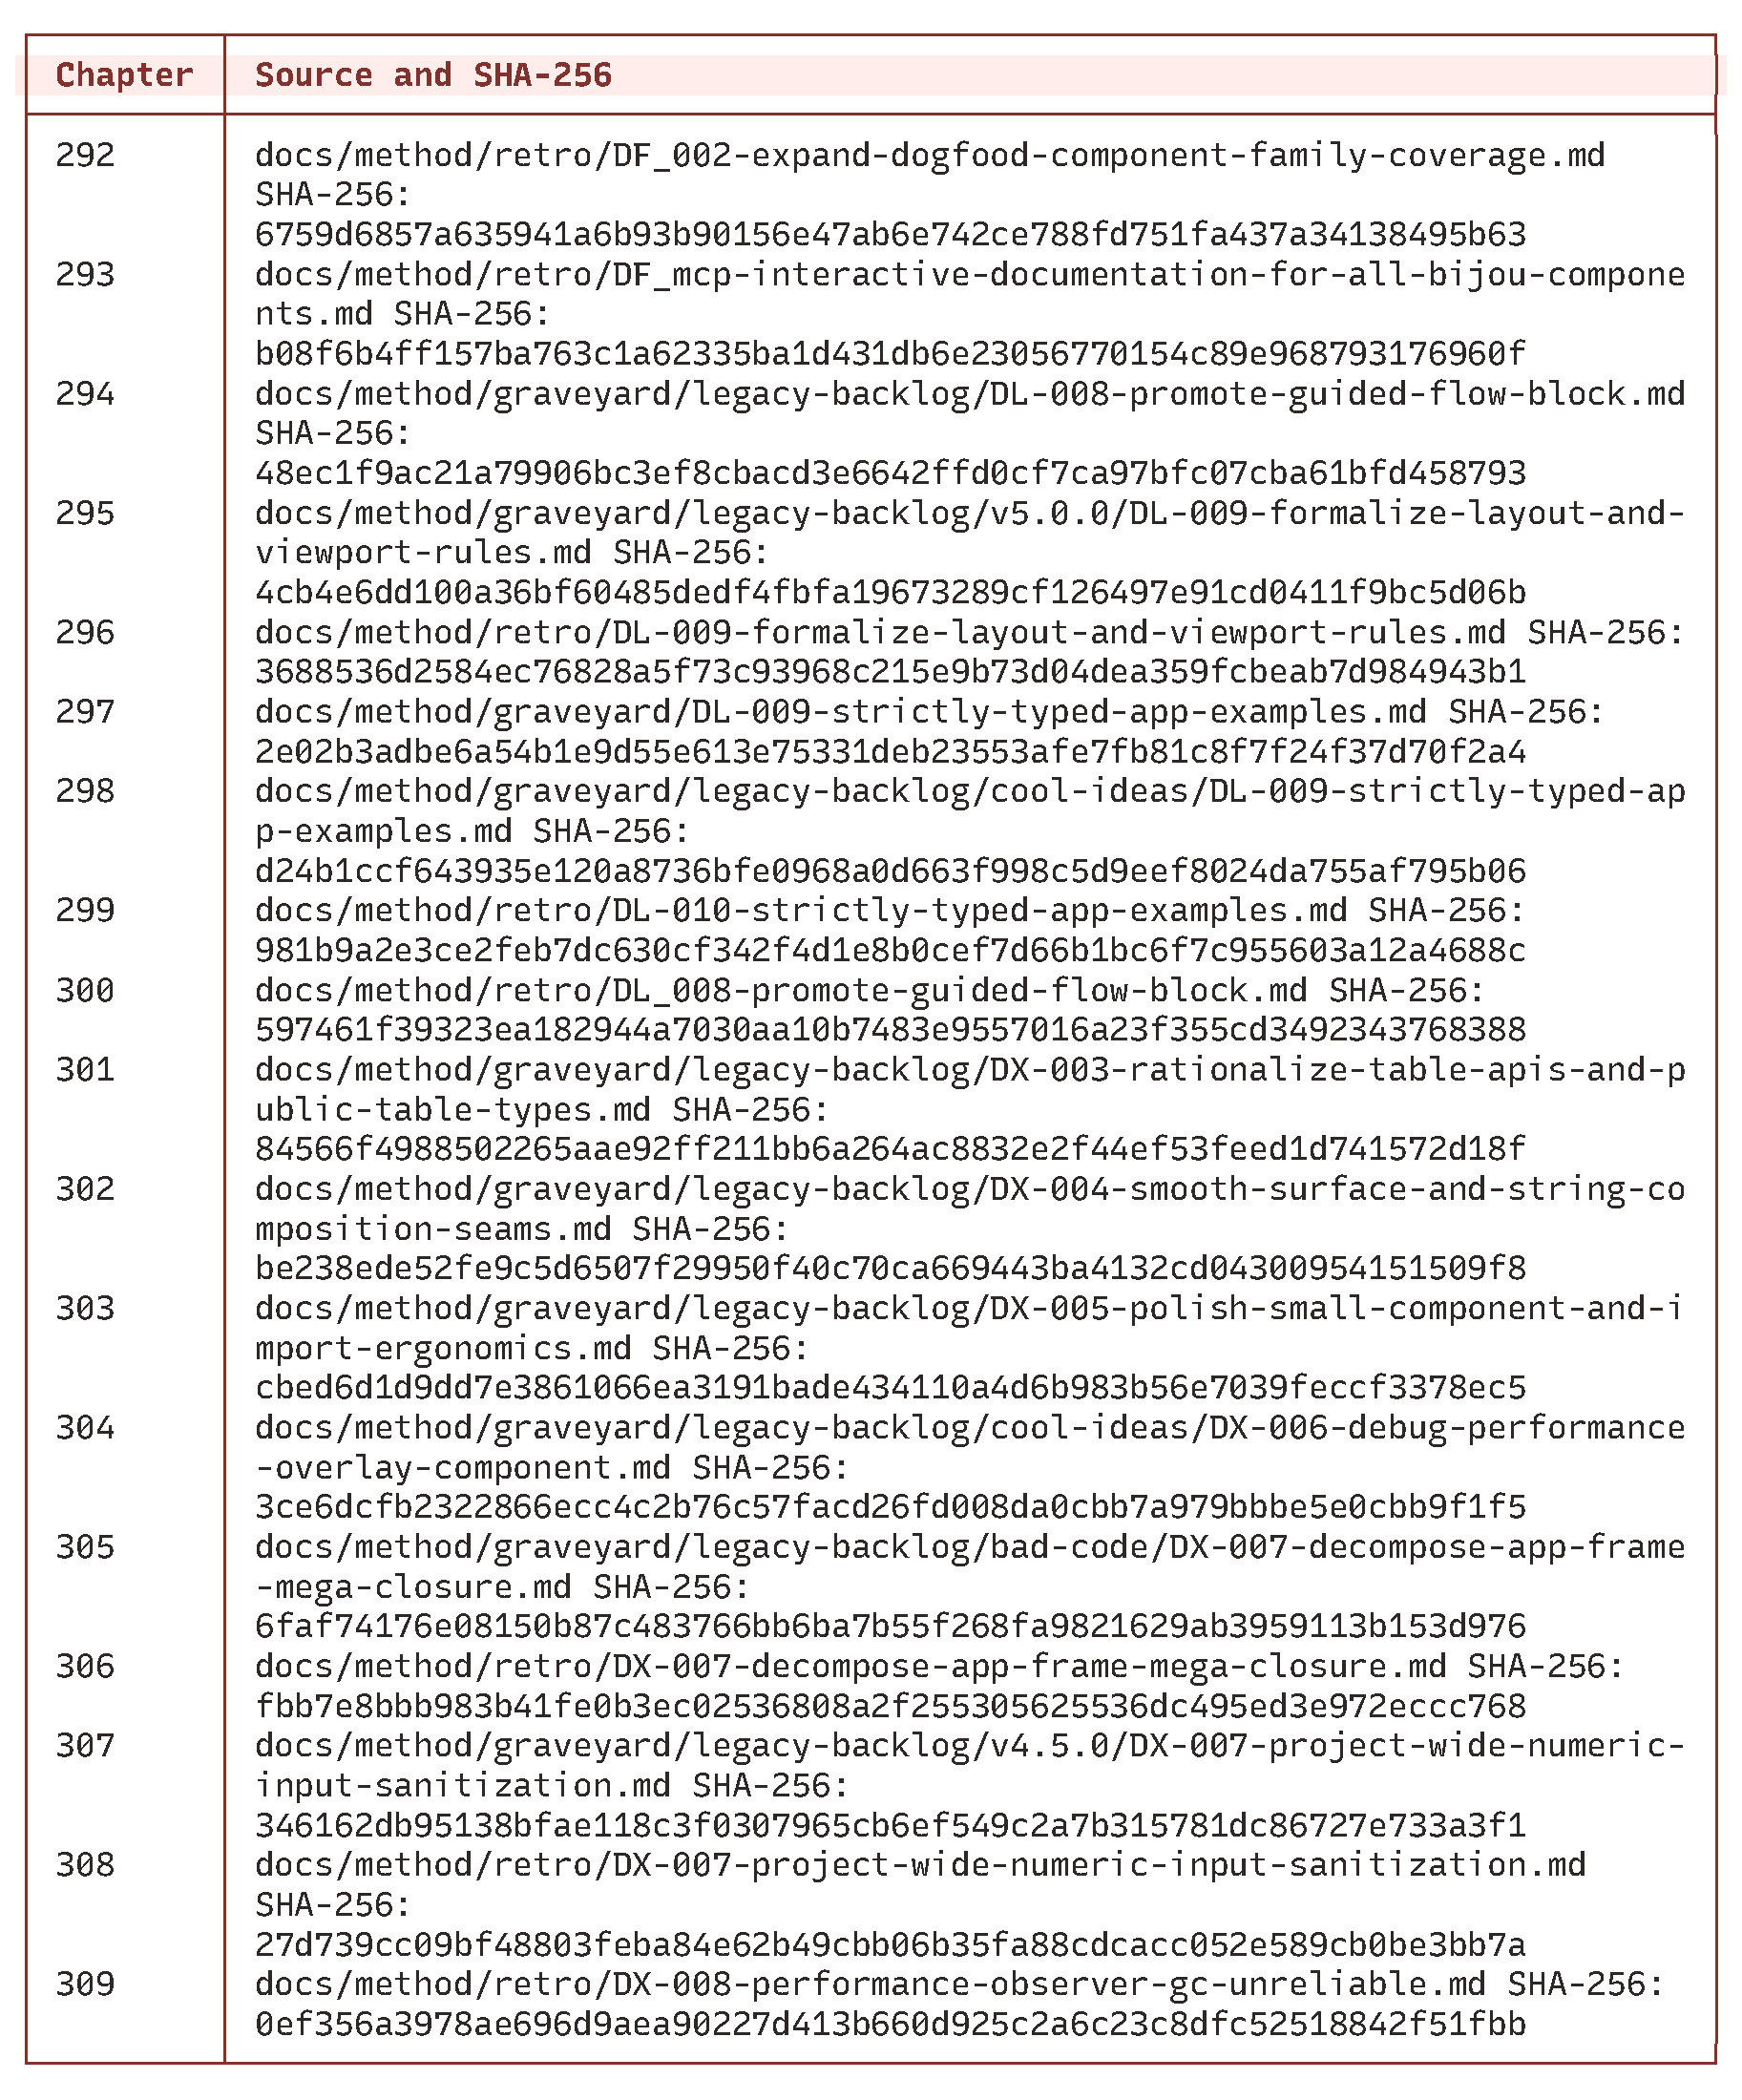
\includegraphics[width=\linewidth]{figures/tables/source-inventory-g1-14.pdf}
\par\smallskip{\scriptsize\color{BookMuted}Rows 292–309. Actual Bijou table component.}
\end{center}
\par\medskip
\begin{center}
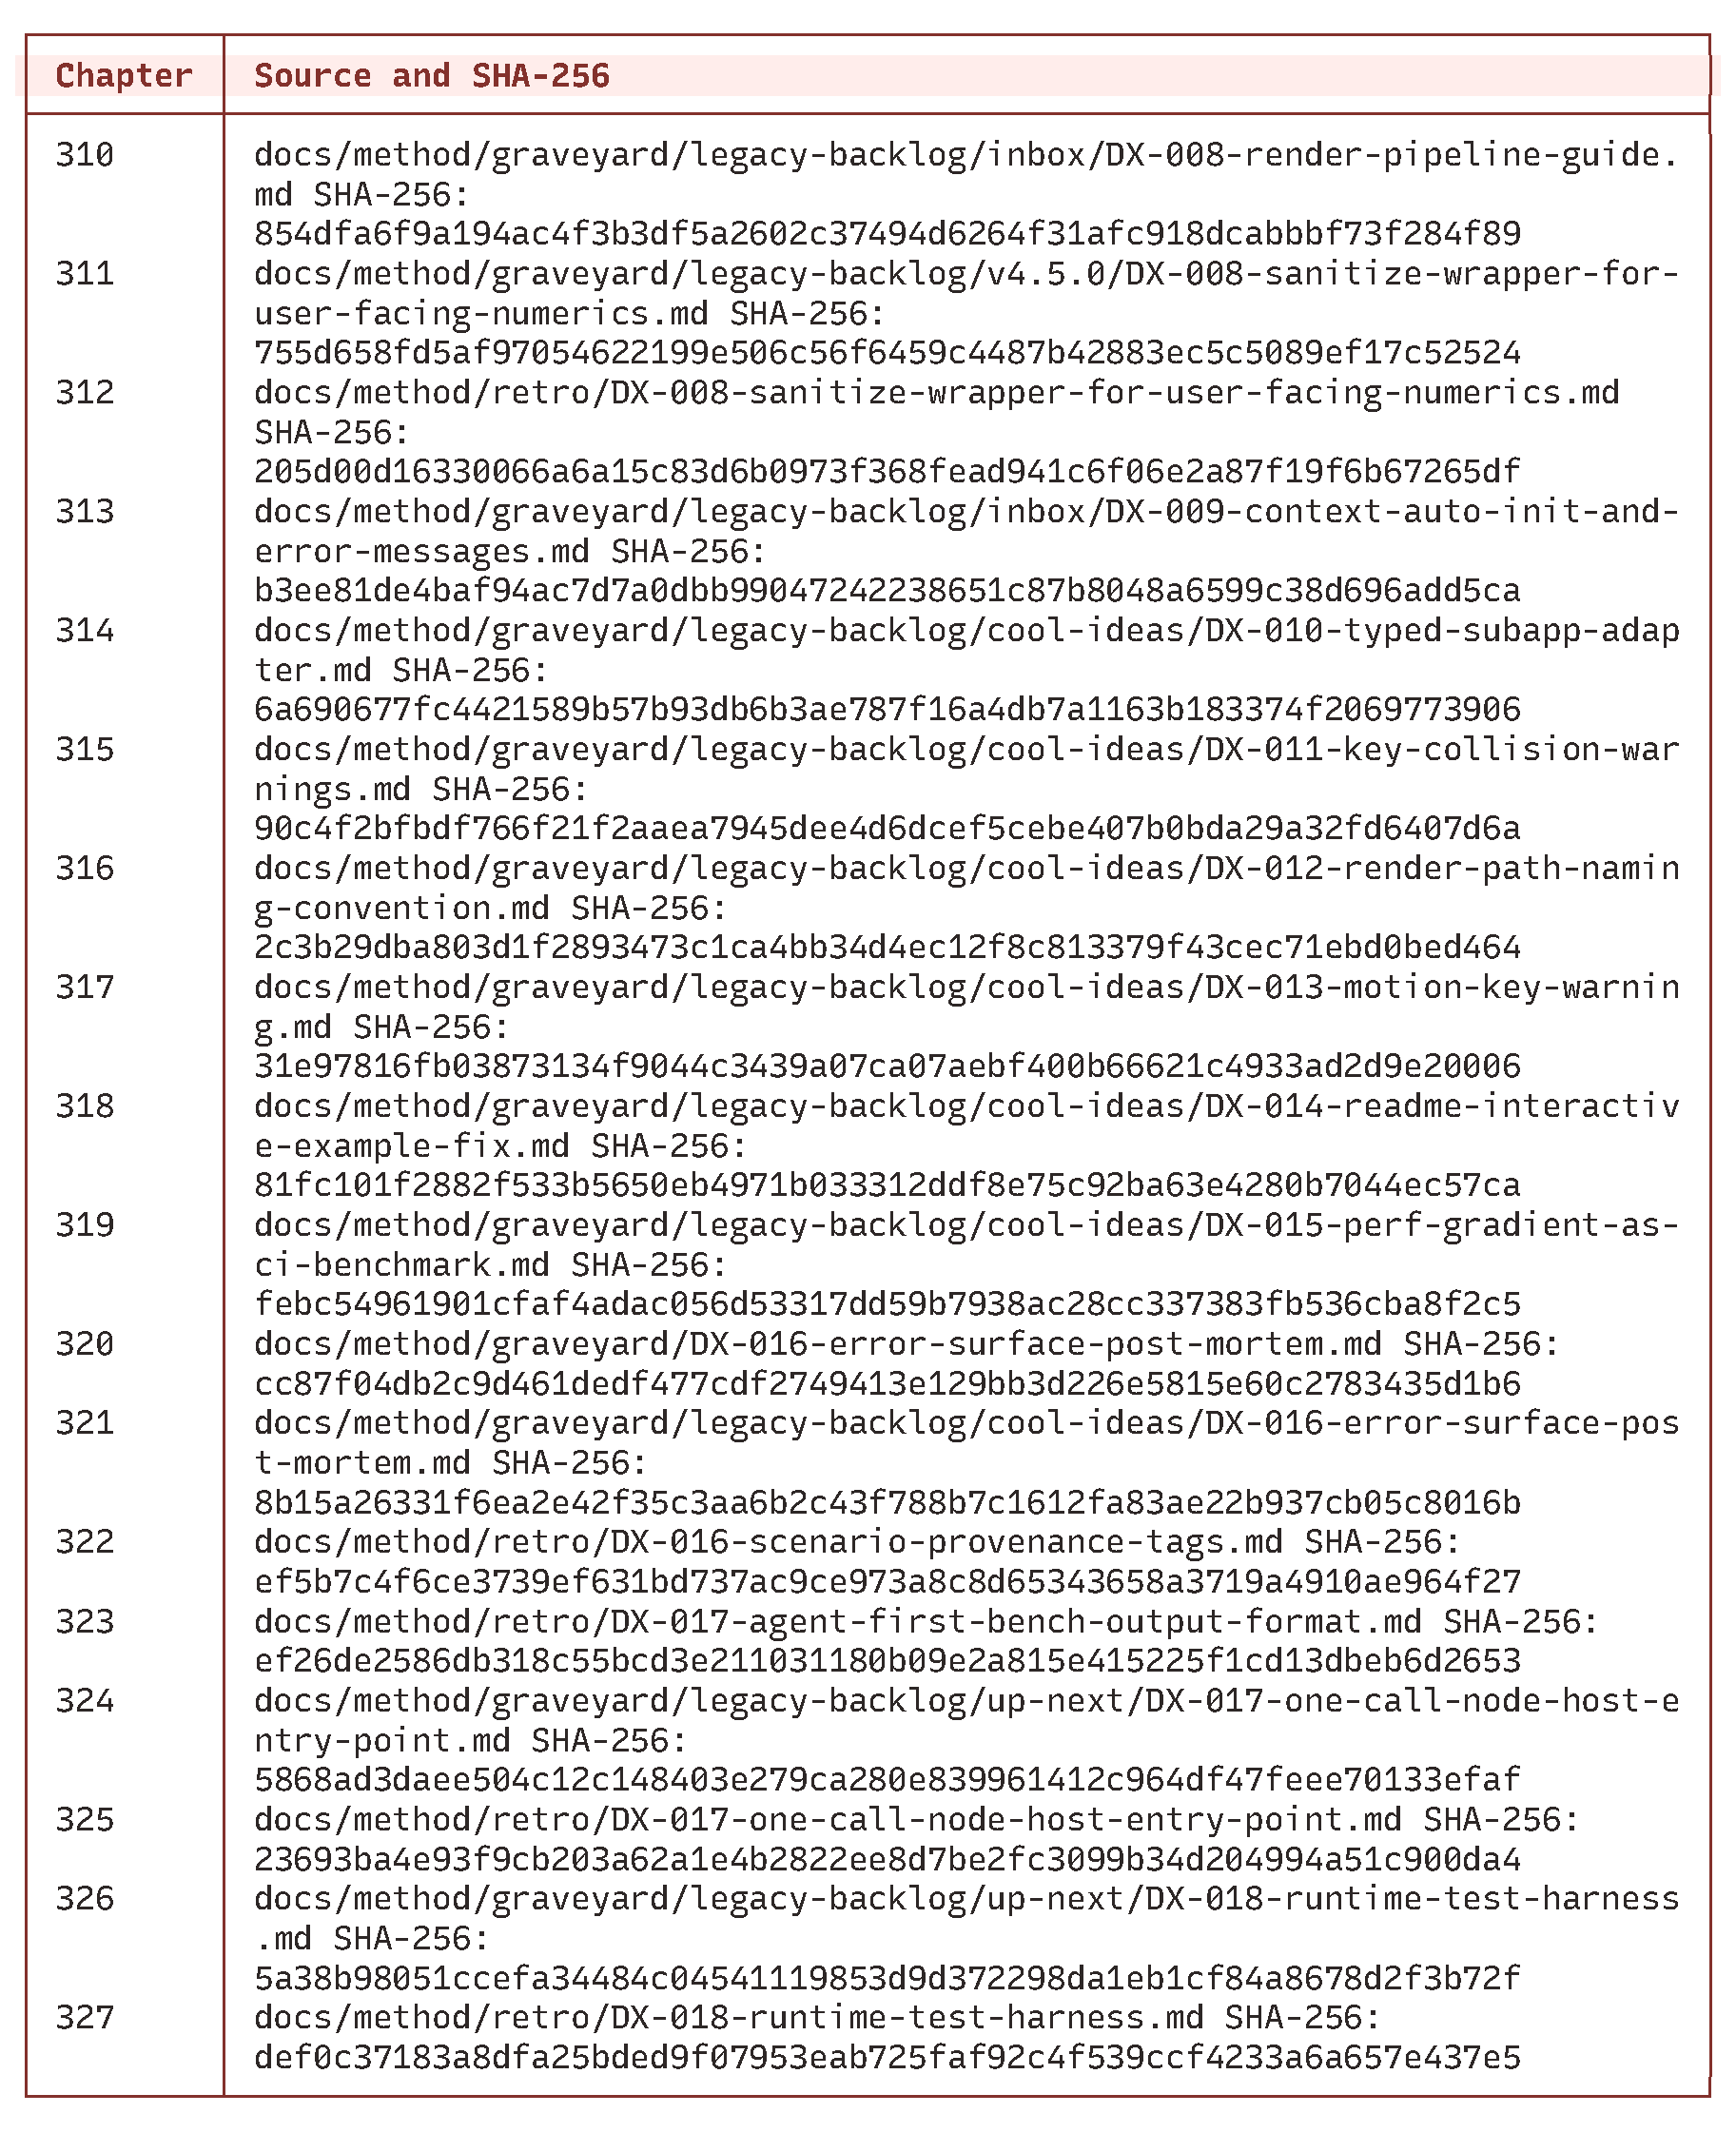
\includegraphics[width=\linewidth]{figures/tables/source-inventory-g1-15.pdf}
\par\smallskip{\scriptsize\color{BookMuted}Rows 310–327. Actual Bijou table component.}
\end{center}
\par\medskip
\begin{center}
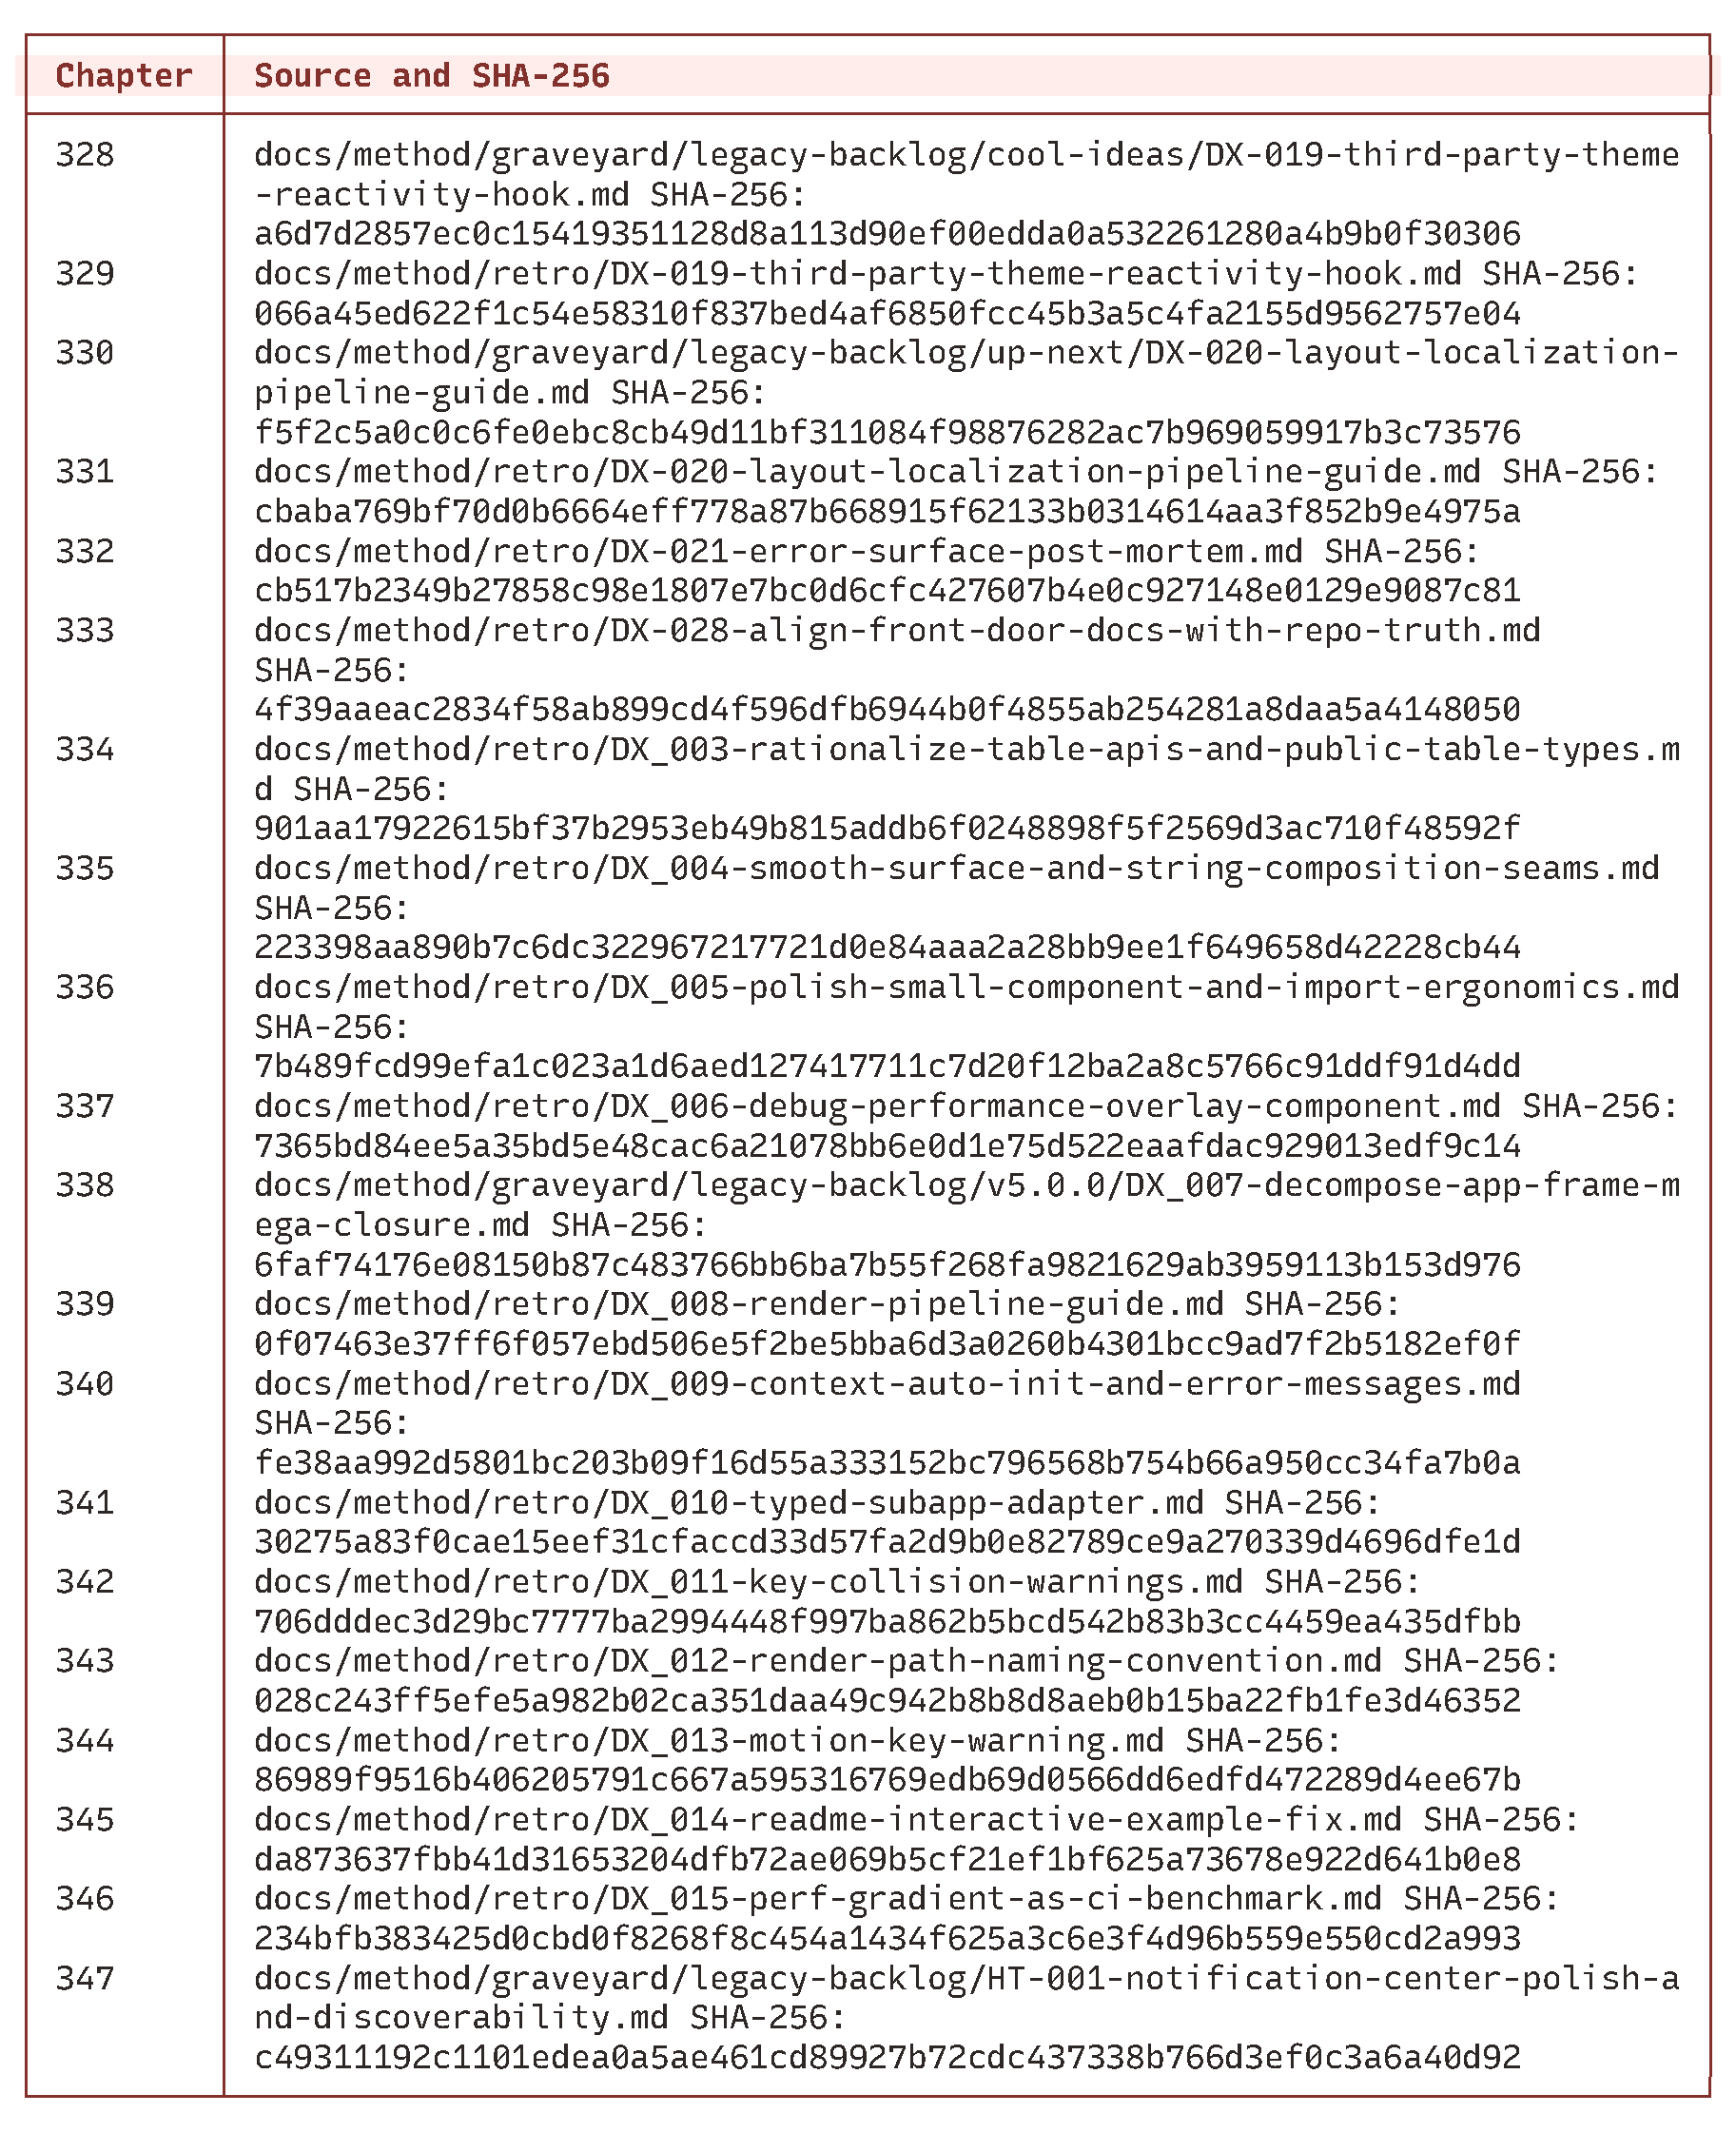
\includegraphics[width=\linewidth]{figures/tables/source-inventory-g1-16.pdf}
\par\smallskip{\scriptsize\color{BookMuted}Rows 328–347. Actual Bijou table component.}
\end{center}
\par\medskip
\begin{center}
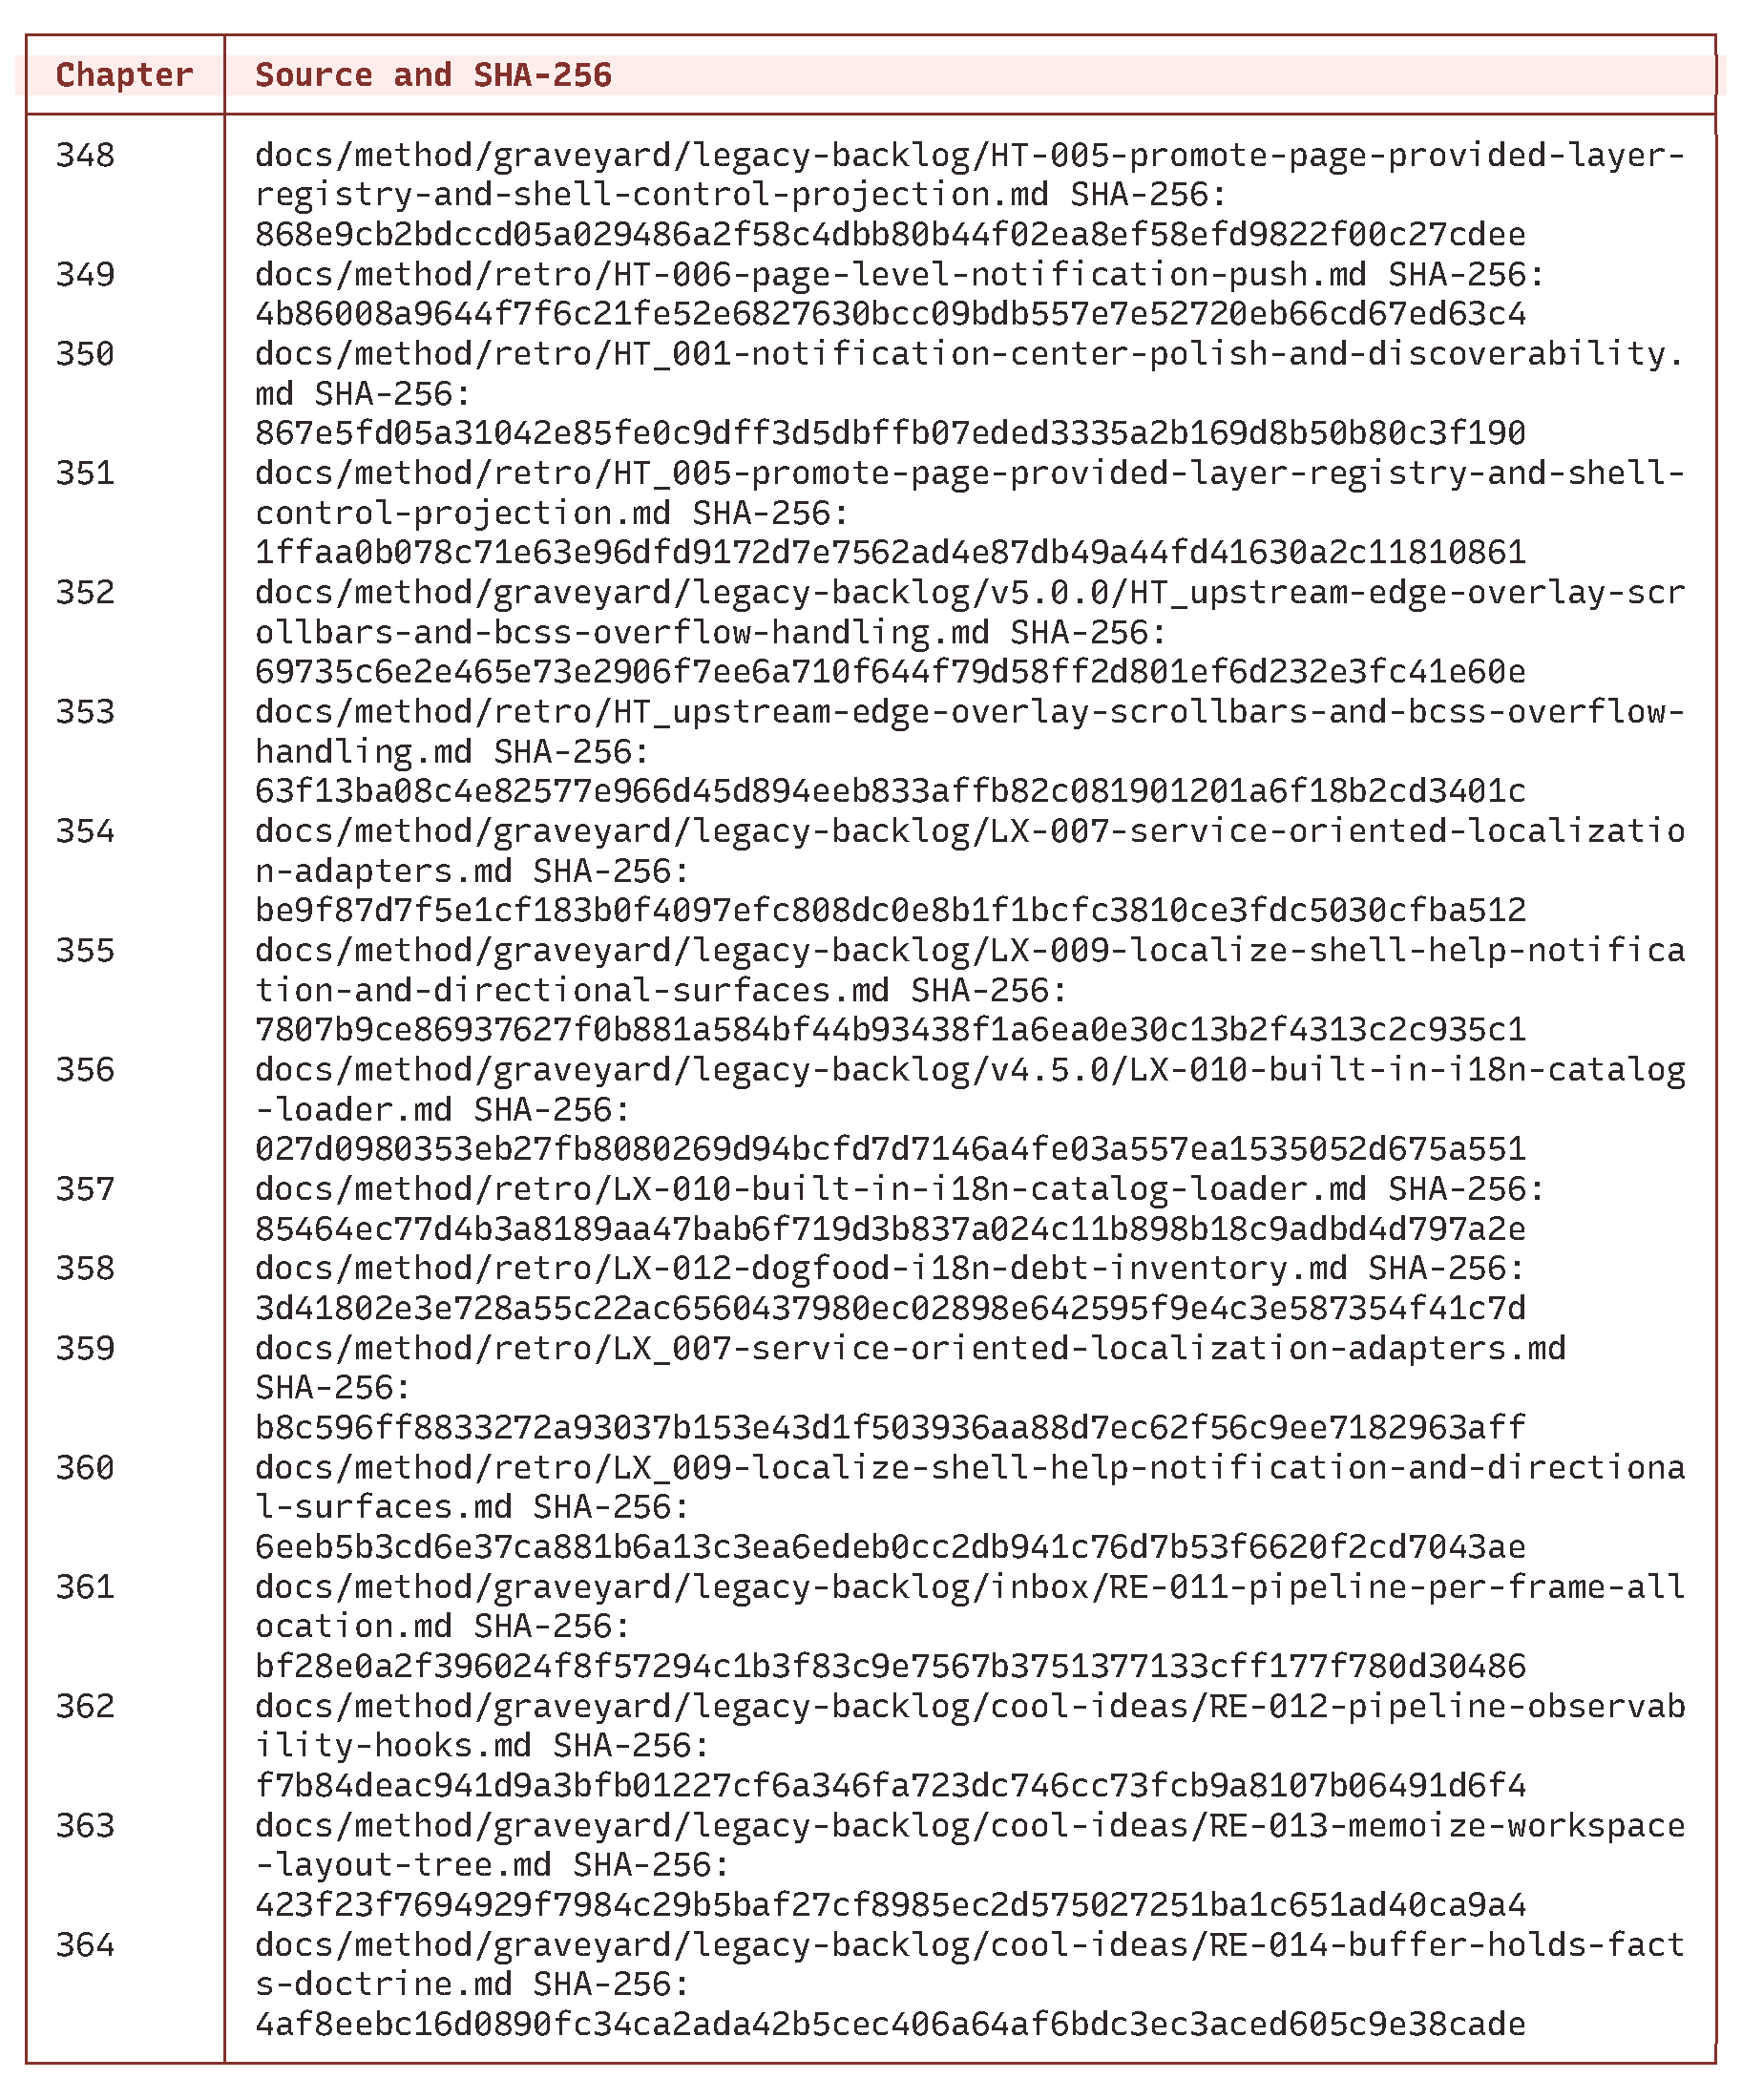
\includegraphics[width=\linewidth]{figures/tables/source-inventory-g1-17.pdf}
\par\smallskip{\scriptsize\color{BookMuted}Rows 348–364. Actual Bijou table component.}
\end{center}
\par\medskip
\begin{center}
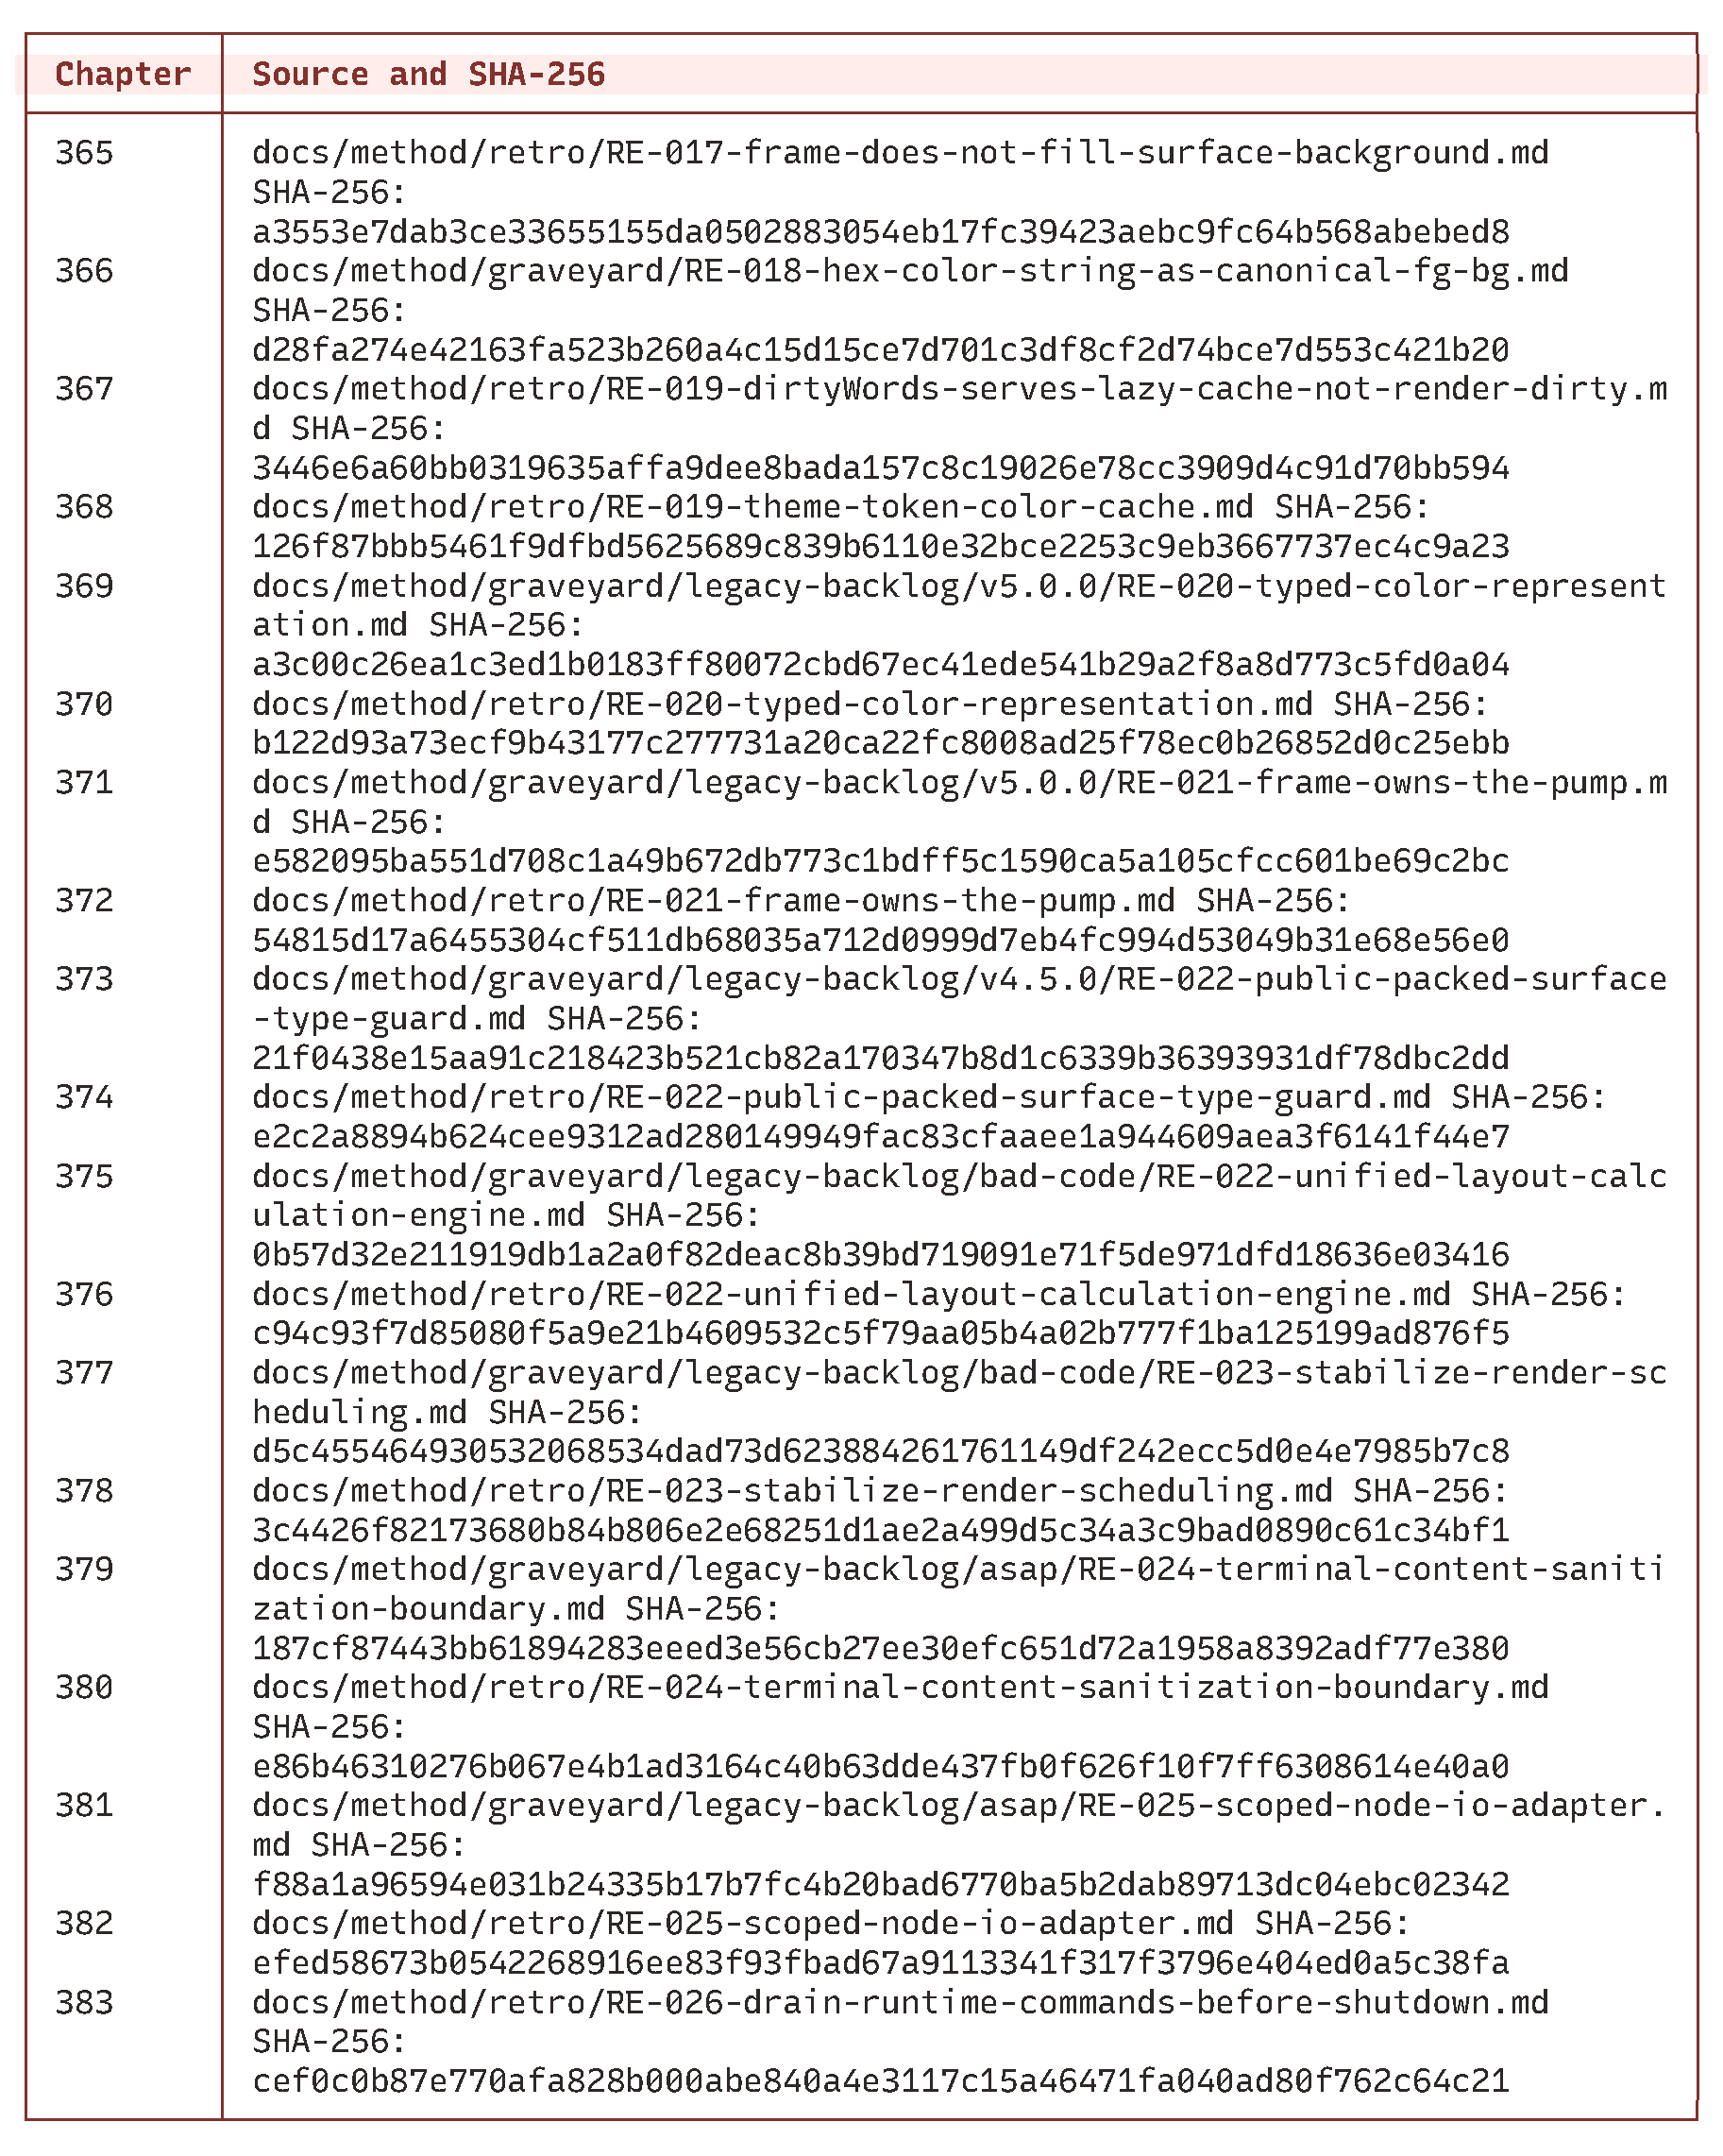
\includegraphics[width=\linewidth]{figures/tables/source-inventory-g1-18.pdf}
\par\smallskip{\scriptsize\color{BookMuted}Rows 365–383. Actual Bijou table component.}
\end{center}
\par\medskip
\begin{center}
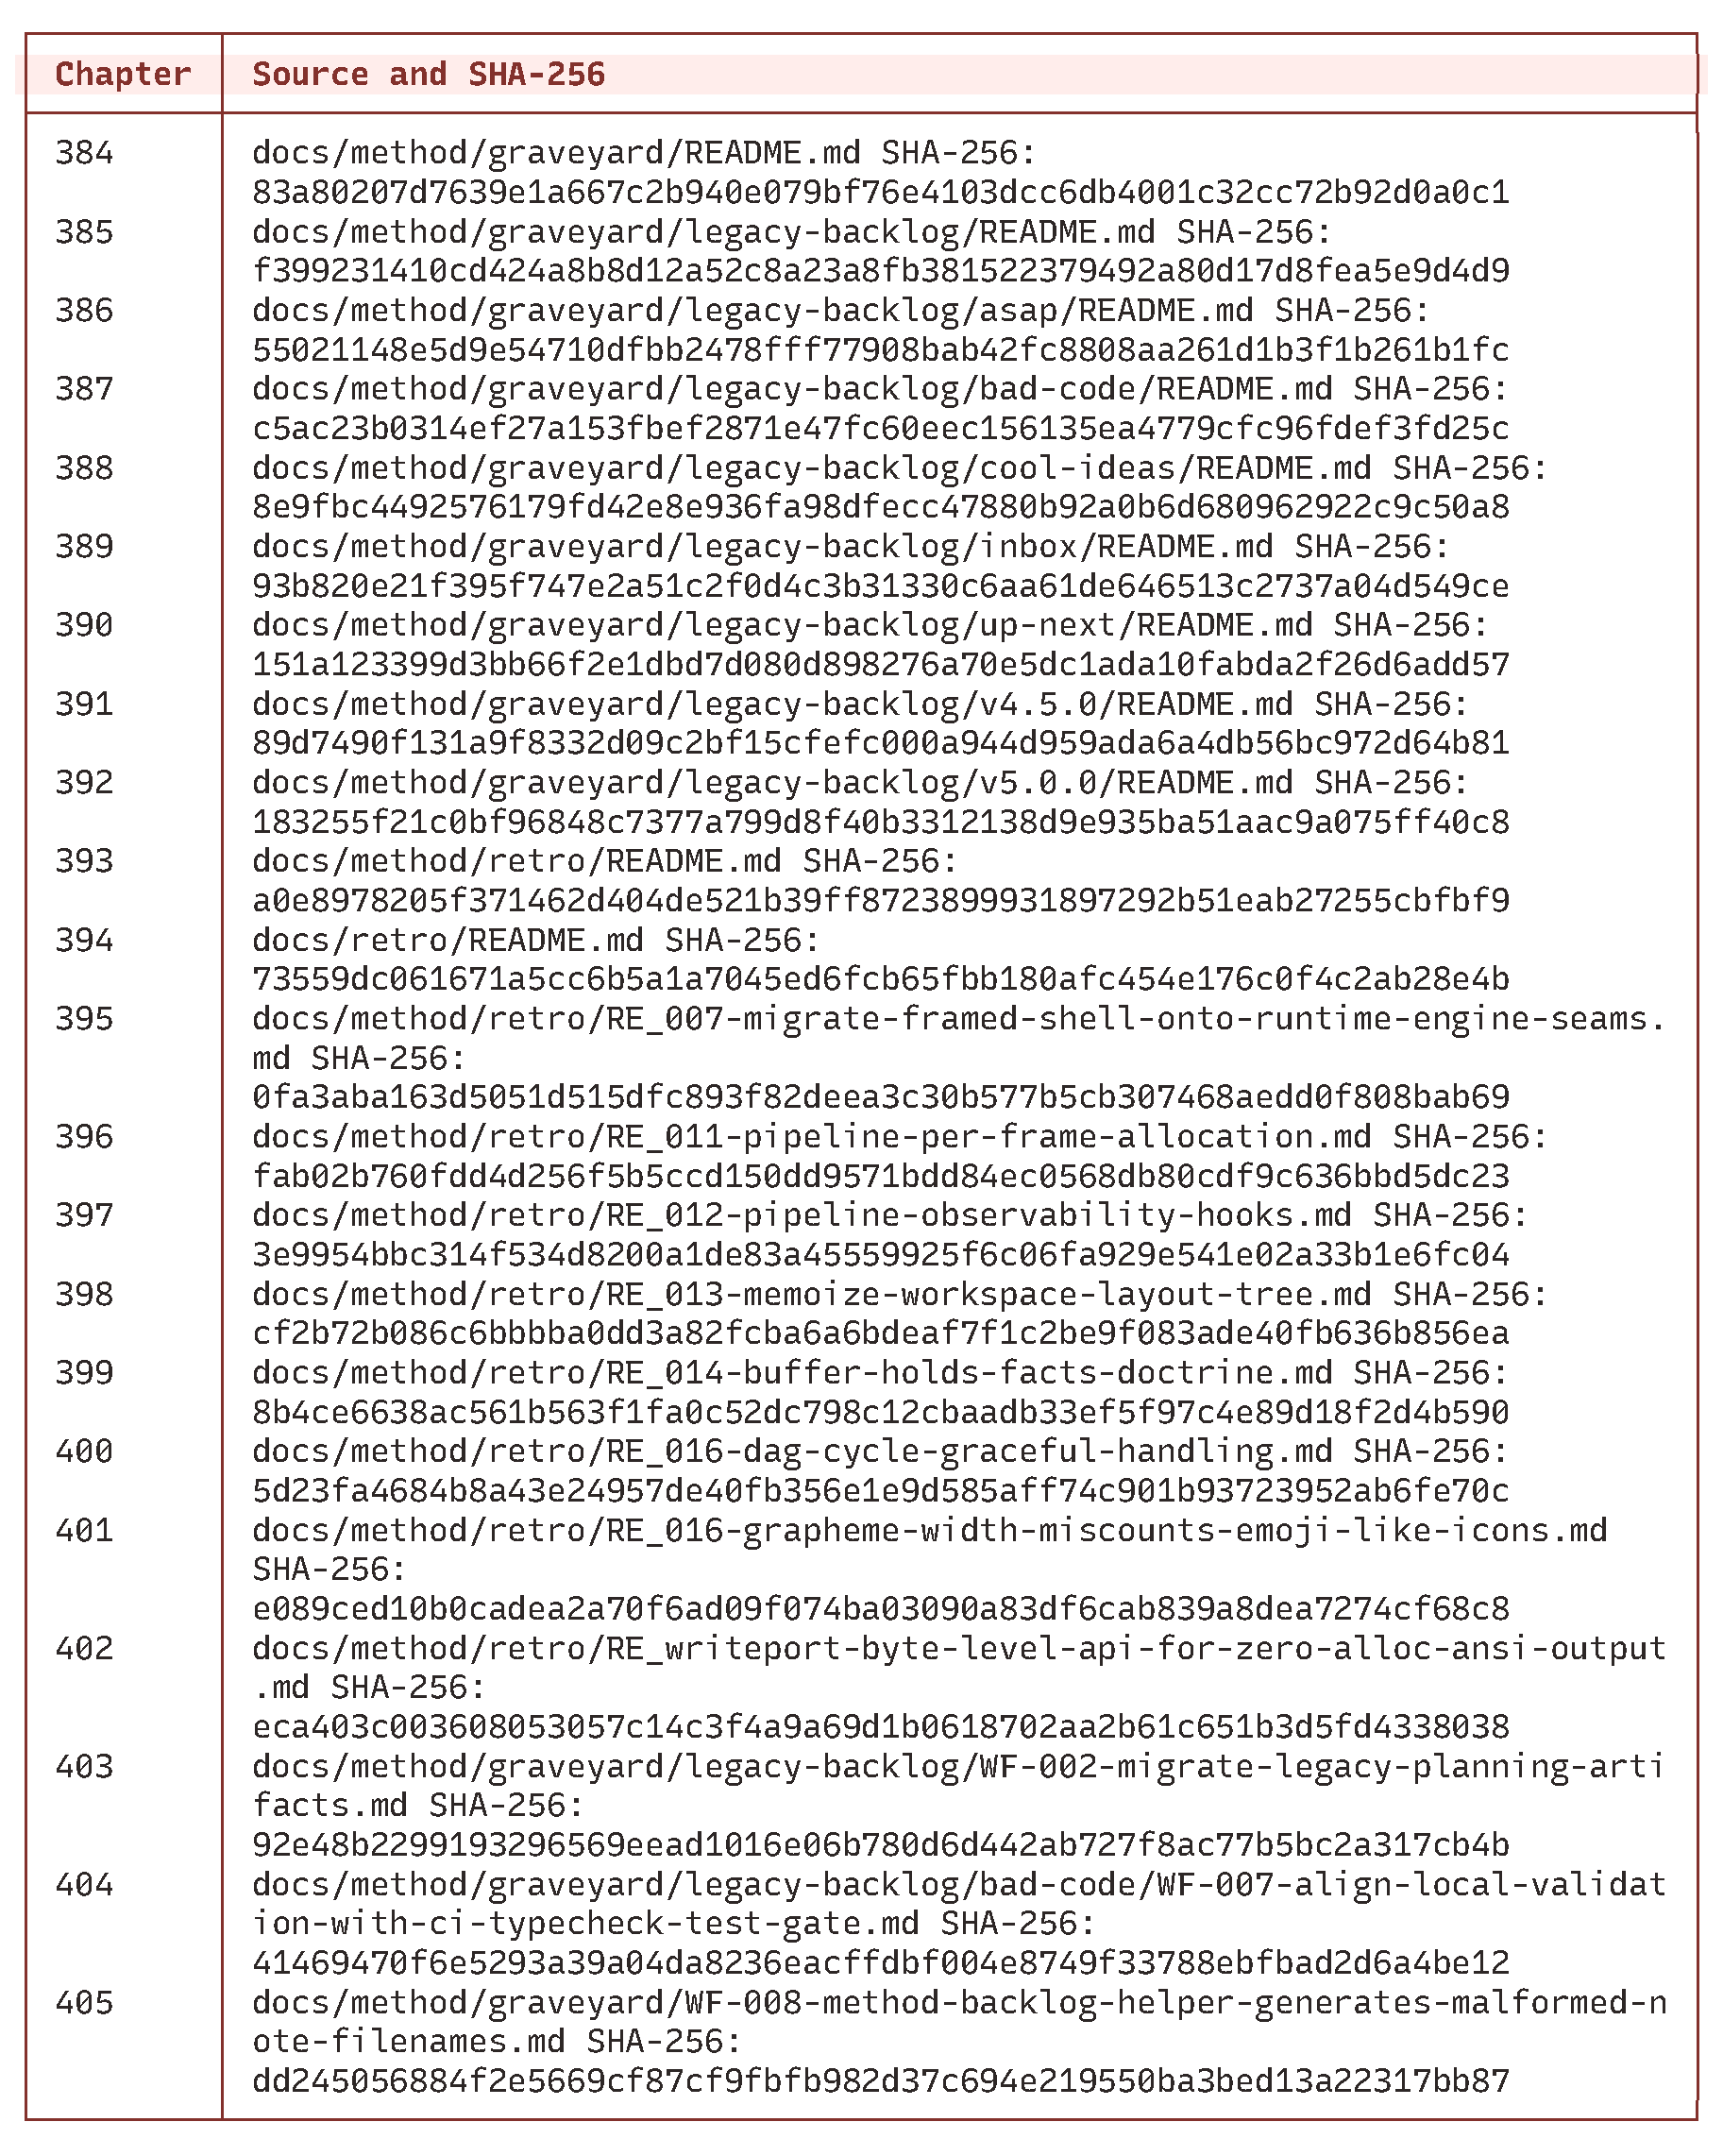
\includegraphics[width=\linewidth]{figures/tables/source-inventory-g1-19.pdf}
\par\smallskip{\scriptsize\color{BookMuted}Rows 384–405. Actual Bijou table component.}
\end{center}
\par\medskip
\begin{center}
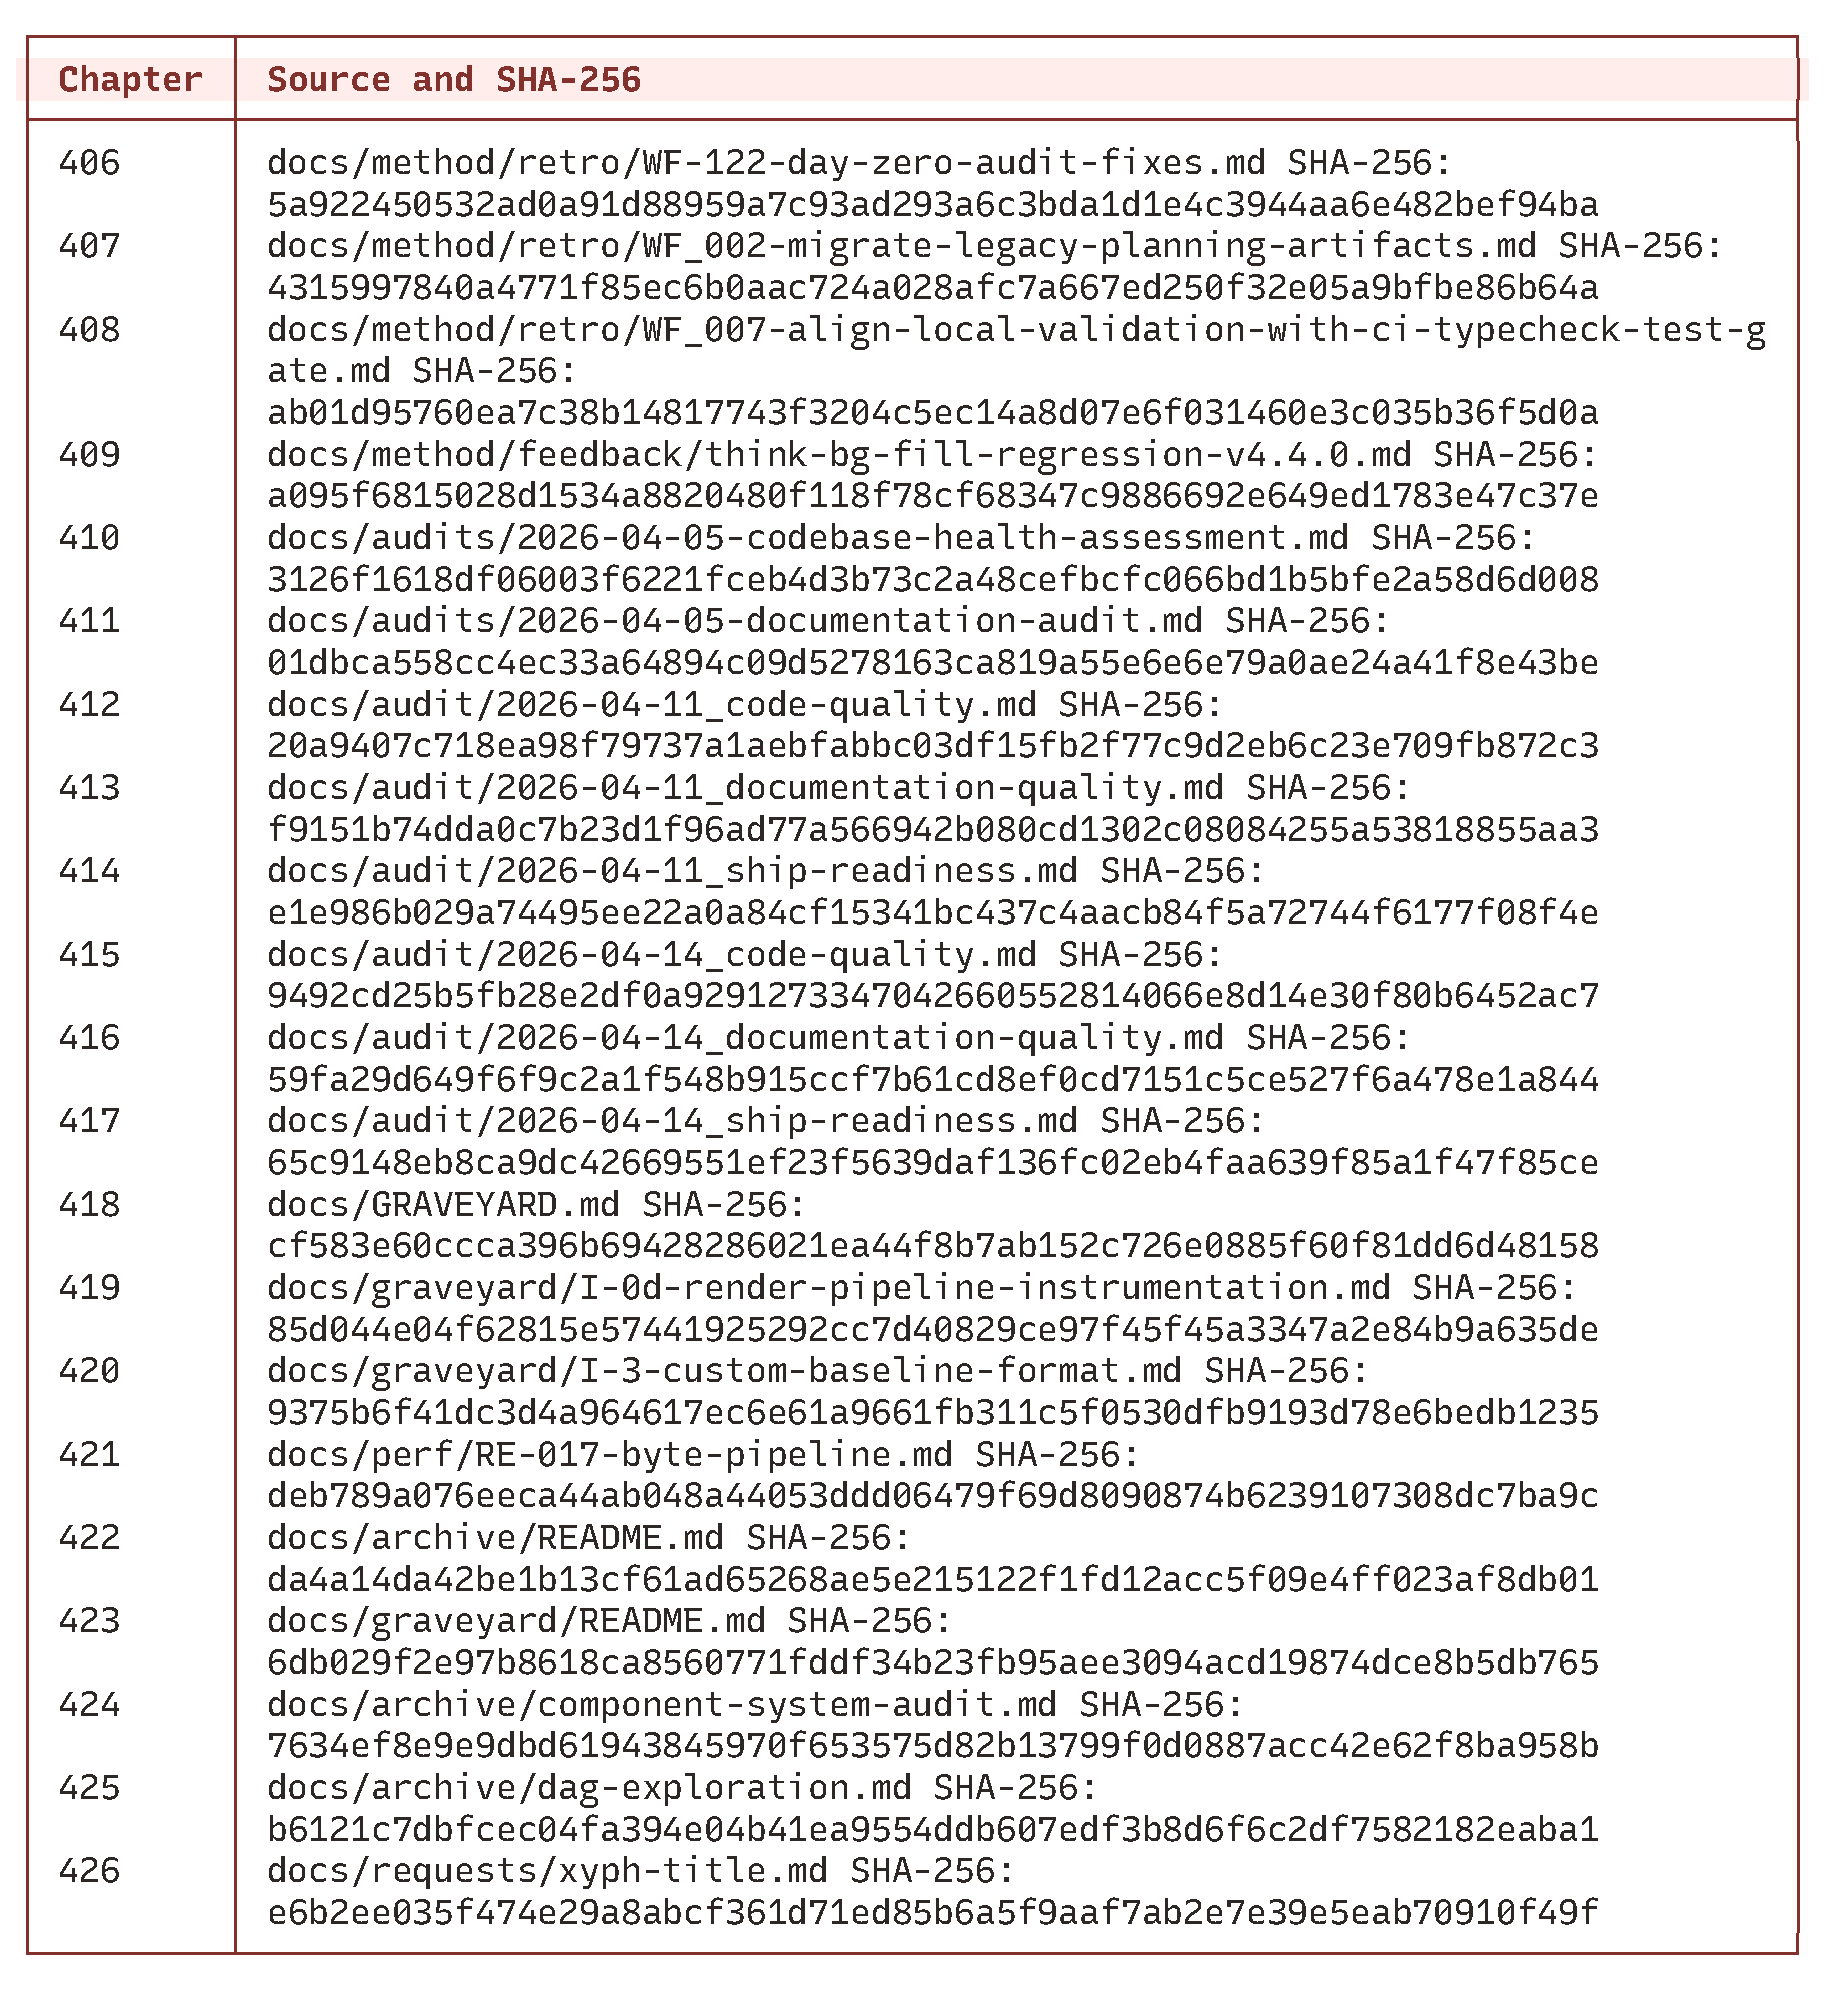
\includegraphics[width=\linewidth]{figures/tables/source-inventory-g1-20.pdf}
\par\smallskip{\scriptsize\color{BookMuted}Rows 406–426. Actual Bijou table component.}
\end{center}

%
\else
\chapter{Sources and further reading}

The historical source inventory belongs to the separate Design Archive and the complete edition. It accounts for 426 original paths and their hashes. This teaching volume uses the same frozen corpus and shared illustration assets without printing the historical records.

The companion source is fixed to the commit and release recorded on the version page. Its \path{LICENSE}, \path{NOTICE}, \path{VERIFICATION.json}, checkpoints and exercises belong to that edition. Book source manifests identify the cell captures, tables, diagrams, fonts and archived documents. Use the archive when following the history of a design; use the pinned companion when reproducing a workshop.
\fi
